\documentclass[3p,twocolumn,number]{elsarticle}
 
\usepackage{amsmath,amssymb,amsthm}

%% Float placement. Two-column layout with page-wide (starred) floats otherwise
%% produces float-only pages: LaTeX's defaults forbid a page from being more
%% than 70% float. These values let floats share a page with text.
\setcounter{topnumber}{3}
\setcounter{dbltopnumber}{3}
\setcounter{bottomnumber}{2}
\setcounter{totalnumber}{5}
\renewcommand{\topfraction}{0.92}
\renewcommand{\dbltopfraction}{0.92}
\renewcommand{\bottomfraction}{0.6}
\renewcommand{\textfraction}{0.06}
\renewcommand{\floatpagefraction}{0.85}
\renewcommand{\dblfloatpagefraction}{0.85}
\usepackage{graphicx}
\usepackage{booktabs,multirow,array,tabularx}
\usepackage{algorithm,algpseudocode}
\usepackage{dblfloatfix}
\usepackage{xurl}
\usepackage[colorlinks=true,linkcolor=blue!60!black,citecolor=blue!60!black,urlcolor=blue!60!black]{hyperref}
\pdfstringdefDisableCommands{%
  \def\corref#1{}%
  \def\cortext#1{}%
  \def\fnref#1{}%
}
\usepackage{xcolor,caption,subcaption}
\usepackage{enumitem}
\usepackage{pgfplots,pgfplotstable}
\pgfplotsset{compat=1.18}
\usepackage{tikz}
\usetikzlibrary{shapes.geometric,arrows.meta,positioning,calc,decorations.pathreplacing}
 
\setlength{\textfloatsep}{10pt plus 3pt minus 2pt}
\setlength{\floatsep}{8pt plus 3pt minus 2pt}
\setlength{\intextsep}{8pt plus 3pt minus 2pt}
\setlength{\abovecaptionskip}{6pt}
\setlength{\belowcaptionskip}{3pt}
\captionsetup{font=small}
\setlength{\abovedisplayskip}{8pt plus 3pt minus 2pt}
\setlength{\belowdisplayskip}{8pt plus 3pt minus 2pt}
 
%% No \FloatBarrier at section or subsection level. With page-wide floats in a
%% two-column layout a barrier forces constant flushing and leaves pages half
%% empty; measured against this manuscript it cost one page of main text and
%% left two pages with large trailing gaps, while every float landed on exactly
%% the same page without it. The float fractions above keep floats near their
%% references on their own.
 
\renewcommand{\arraystretch}{0.90}
 
\journal{Journal of King Saud University -- Engineering Sciences}
 
\newtheorem{definition}{Definition} \newtheorem{proposition}{Proposition} \newtheorem{remark}{Remark} \newtheorem{observation}{Observation} \newtheorem{corollary}{Corollary}
 
%% --- Notation shortcuts ---
\newcommand{\Rset}{\mathbb{R}}
\newcommand{\sched}{\sigma}
\newcommand{\Tmin}{T_{\min}}
\newcommand{\Tmax}{T_{\max}}
\newcommand{\deadband}{\delta_{\mathrm{db}}}
\newcommand{\Tout}{T_{\mathrm{out}}}
\newcommand{\Cth}{C_{\mathrm{th}}}
\newcommand{\lext}{\lambda_{\mathrm{ext}}}
\newcommand{\lwin}{\lambda_{\mathrm{win}}}
\newcommand{\lij}{\lambda_{ij}}
\newcommand{\Qhvac}{Q_{\mathrm{hvac}}}
\newcommand{\csw}{c_{\mathrm{sw}}}
\newcommand{\Phvac}{P_{\mathrm{hvac}}}
\newcommand{\Jbar}{\bar{J}}
\newcommand{\SAR}{\text{SAR}}
\newcommand{\kWh}{\text{kWh}}
\newcommand{\Liz}[1]{\Lambda_{\mathrm{iz},#1}}
\newcommand{\Tiz}[1]{T_{\mathrm{iz},#1}}
\newcommand{\Qiz}[1]{Q_{\mathrm{iz},#1}}
\newcommand{\taup}{\tau^{+}}
\newcommand{\taum}{\tau^{-}}
 
 
%% ============================================================
\begin{document}
 
\begin{frontmatter}
 
\title{Rule-Constrained PPO for Binary HVAC Scheduling in Saudi Residential
Buildings: Cost Savings, Their Governing Parameters, and an Optimality
Bracket}

\author[tu]{Hamzah Faraj\corref{cor1}}
\ead{[email removed]}
\cortext[cor1]{Corresponding author}
\affiliation[tu]{organization={Department of Science and Technology, Ranyah College, Taif University},
                 city={Taif},
                 postcode={21944},
                 country={Saudi Arabia}}

 
\begin{abstract}
HVAC accounts for up to $70\%$ of residential electricity demand in Saudi
Arabia. This paper formulates cost-optimal binary HVAC scheduling as an
infinite-horizon constrained optimisation in which comfort is a hard
constraint, each switch-on incurs a discrete cost and running time incurs a
tariff-weighted cost, and reports what such a schedule can and cannot save. A
hybrid rule-based reinforcement learning framework (RBRL) combines hard comfort
rules with a proximal policy optimisation agent. Its central result is
negative: under the rule layer the learned policy reproduces a bare hysteresis
rule exactly, with identical per-window costs, in nine of ten runs across
Riyadh and Jeddah (the tenth is $0.3\%$ dearer), and a corollary of the
complete-cycle structure explains why---at matched comfort and constant
disturbance that hysteresis is already cost-optimal in its class.

Three climates (Riyadh, Jeddah, Taif) are evaluated on a $[22,24]\,^\circ$C
occupied band, with every controller matched in every held-out window to that
window's own baseline mean occupied temperature, so no arm can have bought its
saving with temperature. A tuned two-parameter thermostat reduces cost by
$9.3\pm1.6\%$, $9.3\pm1.4\%$ and $4.6\pm3.6\%$---significant against the
baseline on the seven paired windows (exact Wilcoxon $p=0.016$, $0.016$ and
$0.031$), and $9.3\%$ at a switch-on cost of $0.15\,\SAR$, falling to
approximately $7.7\%$ at the $0.114\,\SAR$ upper value that the wear
derivation reported here supports. RBRL reaches only $5.7\%$ in
Riyadh, and a $24\,$h receding-horizon controller is statistically
indistinguishable from the tuned thermostat in Riyadh ($p=0.94$) and
significantly below it in Jeddah ($p=0.047$); only at a $48\,$h horizon, the
scale of the plant's $56\,$h time constant, does it draw level. A Lagrangian relaxation brackets what clairvoyance is worth between
an attainable $18.1$, $17.8$ and $15.0\%$ and a bound of $19.8$, $19.5$ and
$20.2\%$ that no mean-matched schedule can beat. Compressor starts fall
$7.5$--$16.7\%$ while energy moves by $-0.3\%$ to $+0.5\%$, so the saving is a
switching saving, as a duty-cycle identity derived here requires---and is
therefore deferred compressor wear, not a lower bill. Two parameters
govern it, neither algorithmic: the tariff, since the percentage falls as the
energy price rises while the absolute saving holds near
$0.10\,\SAR$/zone/day, and the comparator's deadband, an unmeasured hardware
constant that reverses the sign of the result at $1.25\,^\circ$C. Integration
is exact, so no stability condition arises; what replaces it is an actuation
condition, $\Qhvac\Delta t/\Cth\le\deadband$, in which $\deadband$ is the
controller's deadband, not the comfort band, and which an hourly
interval violates.
\end{abstract}
 
\begin{keyword}
HVAC scheduling \sep constrained deep reinforcement learning \sep proximal policy
optimisation \sep building energy management \sep step-wise electricity tariff
\sep thermal comfort \sep Saudi Arabia \sep load scheduling
\end{keyword}
 
\end{frontmatter}
 
%% ============================================================
\section{Introduction}
\label{sec:intro}
 
Buildings consume approximately 40\% of global final energy, with HVAC systems accounting for roughly half that figure~\cite{PerezLombard2008}.
In Saudi Arabia the challenge is particularly acute: residential buildings alone consume $\approx$50\% of national electricity, and air conditioning represents up to 70\% of residential demand~\cite{AlHomoud2021}, \cite{Krarti2020}.
Achieving the efficiency targets of Saudi Vision~2030 therefore requires intelligent, adaptive control of residential HVAC systems~\cite{Belaid2025}.
 
\subsection{Motivation}
 
The prevalent residential control strategy is the automatic thermostat: it switches on when a room exceeds an upper setpoint and off when it returns, with no tariff awareness and no inter-zone coordination.
Where the residential tariff places a price boundary inside the billing month~\cite{Nahiduzzaman2023,SEC2024}, this unawareness carries a measurable cost premium.
Model Predictive Control (MPC) addresses tariff awareness but requires a mixed-integer programme at each step, which limits embedded deployment at scale~\cite{Risbeck2017}.
Reinforcement Learning (RL) offers a model-free alternative~\cite{AlSayed2024}, \cite{Biemann2021}, \cite{Azuatalam2020}, yet pure RL agents can violate comfort constraints during exploration~\cite{Xu2025}.
Hybrid rule-RL approaches combine hard safety rules with RL adaptability~\cite{Xu2025}, \cite{Solinas2024}. The closest prior work is the present author's physics-informed PPO framework for Saudi residential split units under the same tariff~\cite{Faraj2026}, which enforces comfort through a soft physics penalty and reports no optimality certificate; Section~\ref{subsec:gap} sets out what the present study adds to it and what it takes from it.
This paper closes that gap.
 
\subsection{Contributions}
 
Five contributions are made.
(C1)~A formally constrained binary optimisation model of the HVAC scheduling problem across three zone topologies, cast as an \emph{infinite time horizon} problem with an explicit three-condition definition of schedule optimality and a limit-average cost objective.
(C2)~A theoretical connection between the single-zone constant-tariff subproblem and Simple Linear Hybrid Automata~\cite{Mousa2016}, which characterises the structure of an optimal schedule in the tractable special case and identifies the three features---multi-zone coupling, a consumption-dependent per-mode cost rate and time-varying disturbances---that take the full formulation outside that class, motivating RBRL as a practical approximation.
(C3)~The RBRL framework, in which hard rules enforce the comfort band at every decision interval and a PPO agent minimises tariff cost, with adjacent zone temperatures in the agent state to enable inter-zone coordination, together with its honest evaluation, whose central result is negative: on the single-zone instance the learned component recovers no cost beyond the rule-induced hysteresis, and Corollary~\ref{cor:rules_sufficient} proves why none was there to recover.
(C4)~A tariff comparison establishing that the saving available to any controller is governed by the ratio of the per-start charge to the energy price, and quantifying it across the superseded, in-force and announced Saudi residential schedules, with quantified cost savings for three climates on a held-out window set, and with the saving mechanism separated into its tariff-arbitrage and cycling-reduction components. No energy saving is claimed: for the plant modelled here, periodic-steady-state consumption is fixed by the envelope balance and the mean zone temperature, so scheduling redistributes demand in time and reduces cycling, not total energy (Remark~\ref{rem:energy_identity}).
(C5)~An optimality bracket for the instance studied, a per-window-matched attainable clairvoyant schedule below a grid-converged Lagrangian dual bound that no mean-matched schedule can beat, so that every reported saving is read against what was available, not against zero, inside a unified state-of-the-art comparison and ablation study with worked numerical examples following the running-example style of Mousa et al.~\cite{Mousa2016}.
 
Section~\ref{sec:litreview} surveys the related literature.
Section~\ref{sec:prelim} defines the thermal and cost models.
Section~\ref{sec:schedule} formalises the constrained optimisation.
Section~\ref{sec:method} presents RBRL.
Section~\ref{sec:casestudy} characterises the three climates.
Section~\ref{sec:sim} describes the simulation setup.
Section~\ref{sec:results} reports results.
Section~\ref{sec:analysis} benchmarks and ablates.
Section~\ref{sec:discussion} interprets the findings.
Section~\ref{sec:conclusion} concludes.
 
\section{Literature Review}
\label{sec:litreview}
 
The gap set out above has four components: binary actuation, hard comfort
enforcement, an optimality reference, and Saudi climate and tariff coverage.
This review takes each in turn, prioritising publications from 2022 onward.
Earlier works are included only where they represent foundational or seminal contributions essential for context: the global buildings energy baseline~\cite{PerezLombard2008}, the RC model identification framework~\cite{Bacher2011}, the MPC-MILP formulation for HVAC~\cite{Risbeck2017}, and the SLHA optimal control theory~\cite{Mousa2016}, \cite{Mousa2017}.
 
\subsection{Building Energy in Saudi Arabia}
 
Al-Homoud and Krarti~\cite{AlHomoud2021} attribute the Kingdom's residential
demand to an extreme hot climate, low energy-awareness among occupants, and a
historically subsidised tariff that removed price incentives for conservation.
Saudi residential electricity is priced on a step-wise schedule~\cite{Nahiduzzaman2023,SEC2024}: under the four-tier schedule in force from 2016 to 2017 the marginal rate rose six-fold across consumption blocks ($0.05$ to $0.30\,\SAR/\kWh$)~\cite{Nahiduzzaman2023}; the 2018 reform flattened the first three blocks into a single $0.18\,\SAR/\kWh$ band up to $6{,}000\,\kWh$/month and retained a step to $0.30\,\SAR/\kWh$ above~\cite{SEC2024}, repriced to $0.21$ and $0.33\,\SAR/\kWh$ from January~2027~\cite{SaudiEnergy2027}. Accounts above $6{,}000\,\kWh$/month therefore still face a materially higher marginal price.
 
Al-Reshidi et al.~\cite{AlReshidi2024} analysed energy performance across Saudi climate zones and found that compliance with the 2018 Saudi Building Code (SBC)~\cite{Alayed2021} reduces envelope heat gain substantially, yet residential energy demand remains high because HVAC control strategies are unchanged.
Bela\"{\i}d and Mikayilov~\cite{Belaid2024} further showed that the direct rebound effect in Saudi residential electricity consumption partially offsets efficiency gains from appliance upgrades, reinforcing the need for scheduling-level optimisation beyond hardware replacement alone.
 
\subsection{HVAC Control: From Thermostats to Reinforcement Learning}
 
The standard residential HVAC controller is a fixed-setpoint thermostat: it switches on when the zone exceeds an upper setpoint and off when it returns to a lower one.
This approach provides thermal comfort but offers no awareness of electricity tariffs, occupancy patterns, or weather forecasts~\cite{Alotaibi2024}.
 
\paragraph{Model Predictive Control (MPC)}
MPC advances beyond thermostats by optimising a cost objective over a rolling prediction horizon, typically formulating a mixed-integer linear programme (MILP)~\cite{Risbeck2017}.
Dinh et al.~\cite{Dinh2022} demonstrated a MILP-based day-ahead scheduling framework for community-level energy management, reporting significant savings but requiring centralised computation.
Drgoňa et al.~\cite{Drgona2020} review MPC for buildings, documenting savings of 10--30\% relative to rule-based control under idealised conditions.
MILP complexity grows with the number of binary variables and zone count and needs an on-line solver at each step, which is the standing objection to MPC for multi-zone residential deployment. On the single-zone instance of this paper the objection does not bite, and a receding-horizon controller is reported in Section~\ref{subsec:abl_component} as the causal comparator: its saving at a $24\,$h horizon ($5.9$--$8.4\%$) falls \emph{below} the $10$--$30\%$ range Drgo\v{n}a et al.\ document for idealised conditions---iso-comfort matching and held-out evaluation, neither standard in that literature, both reduce the number---and its collapse at $6\,$h locates where that range comes from.
 
\paragraph{Reinforcement Learning}
RL-based approaches learn a control policy through interaction with the building environment, without requiring an explicit model.
Azuatalam et al.~\cite{Azuatalam2020} demonstrated that Q-learning achieves 22\% energy saving over a thermostat in a whole-building simulation.
Biemann et al.~\cite{Biemann2021} compared Soft Actor-Critic (SAC) and TD3 agents for continuous HVAC control, showing improvements exceeding 10\% over rule-based baselines.
More recent work has scaled to multi-zone buildings: Du et al.~\cite{Du2021b} applied DDPG to a multi-zone residential setting and reported 15\% savings; Du et al.~\cite{Du2021a} extended this to multi-task DRL, learning temperature and energy objectives jointly.
Li et al.~\cite{Li2024MZ} showed that including inter-zone temperature observations in the agent state is critical for avoiding cascading heating load in adjacent zones.
 
Recent work expands the scope along three axes: model-based and multi-agent
DRL for multi-zone buildings~\cite{Ding2024,Liu2024} and transfer learning
across buildings~\cite{Hou2024}. Most relevant here, Manjavacas et
al.~\cite{Manjavacas2024} compared deep RL algorithms empirically for HVAC
control and found PPO matching SAC at lower computational cost, which is the
ground for adopting PPO in this work.
 
\paragraph{Hybrid rule-RL approaches.}
Pure RL agents can violate thermal comfort constraints during exploration, particularly under peak-summer conditions when the zone approaches the comfort boundary rapidly~\cite{Xu2025}.
Hybrid approaches address this by imposing hard safety rules that override the RL agent near constraint boundaries, leaving the agent to optimise within the safe region~\cite{Solinas2024}, \cite{Xu2025}.
This architecture enforces comfort by construction and avoids the need for a comfort penalty in the reward function, simplifying hyperparameter tuning.
 
\subsection{Binary On/Off vs.\ Continuous Modulation}
 
The majority of the RL-HVAC literature targets \emph{continuous} HVAC modulation (variable air volume (VAV) systems or continuous setpoint adjustment), which allows smooth power reduction instead of hard switching~\cite{Wang2024DRL}.
Saudi residential air conditioners are predominantly fixed-capacity split-unit systems with binary on/off operation.
Binary scheduling introduces a discrete switching cost $\csw$ due to compressor start-up stress and a penalty for excessive cycling that reduces equipment lifespan.
Faddel et al.~\cite{Faddel2023} quantified cycling and rebound effects in commercial HVAC scheduling, showing that ignoring switch-on penalties leads to schedules with 20--30\% higher maintenance cost.
Mousa et al.~\cite{Mousa2016} studied a single-variable Simple Linear Hybrid Automaton (SLHA) with per-mode linear running costs and per-switch discrete costs. They showed that an optimal safe schedule over an \emph{infinite} horizon can be computed in deterministic LogSpace, but that the corresponding \emph{finite}-horizon decision problem is NP-complete, and gave a constant-factor approximation and an FPTAS for it. Mousa et al.~\cite{Mousa2017} extended the setting to several continuous variables, establishing NExpTime membership and a PSpace $\varepsilon$-approximation; they prove no hardness result for the multi-dimensional case.
 
\subsection{Multi-Zone Coordination and Cost Model Fidelity}
 
\begin{sloppypar}
Multi-zone buildings introduce an additional complication: inter-zone heat conduction through shared walls couples the thermal dynamics of adjacent zones.
Without coordination, a zone cooled to a low temperature will draw heat from a warm neighbour, triggering unnecessary activations and increasing switching cost.
Xue et al.~\cite{Xue2025} combined GA pre-scheduling with MADDPG for multi-zone coordination, reporting 6.7\% savings over a rule-based baseline.
Li et al.~\cite{Li2024MZ} showed that including inter-zone temperature in the agent state reduces cascade events by up to 12\% in four-zone configurations.
\end{sloppypar}
 
Regarding cost model fidelity, most scheduling studies assume a linear (constant) electricity price~\cite{ElMakroum2023}, \cite{Gonçalves2022}, or a smooth approximation such as an exponential growth function~\cite{Risbeck2017}.
Neither represents a piecewise-constant step-wise tariff explicitly. What such a tariff does and does not create is settled by Proposition~\ref{prop:path} below: it raises the marginal price of the \emph{last} kWh consumed in a billing month, but it gives no incentive to rearrange consumption \emph{within} that month.
To our knowledge, no prior RL or hybrid study has explicitly evaluated the cost of tariff model approximation by training under one model and evaluating under the true step-wise tariff.
 
\subsection{Research Gap}
\label{subsec:gap}
 
Table~\ref{tab:gap} summarises the positioning of the present work.
The nearest neighbour to this study is the present author's own recent work in
this journal~\cite{Faraj2026}, and the relationship is best stated directly.
That paper addresses binary on/off scheduling for Saudi residential split units
under the two-block tariff, with inter-zone thermal coupling, at two building
scales, and with a cost-model sensitivity across step-wise, linear and
exponential tariffs. It enforces comfort through a \emph{soft} physics-informed
reward and a top-$k$ projection, neither of which excludes a violation, and it
establishes \emph{no} optimality certificate. It names as
priority future work a quantification of the remaining optimality gap against
a day-ahead mixed-integer scheduler, a longer-horizon model-predictive
baseline and modern constrained reinforcement learning, and separately, among
its limitations, observes that formal constraint enforcement would provide stronger
safety properties than its top-$k$ projection heuristic does.

The present study takes up both, though not by the route that paper
anticipated. It supplies an optimality certificate, as a Lagrangian bound no
comfort-matched schedule can beat (Section~\ref{subsec:bound}), and it reports
the receding-horizon comparison at $6$ and $24\,$h horizons
(Section~\ref{subsec:abl_component}). It enforces comfort by construction, but
through hard action masking at the rule layer rather than through constrained
policy optimisation, so it answers the safety requirement by a different
mechanism than the one suggested there. It does not quantify that paper's own
optimality gap, which is a different instance. It does not re-derive the multi-zone,
inter-zone-coupling, cost-model or zone-count results
of~\cite{Faraj2026}, which stand, and it confines its own numerical study to a
single zone for the reason given in Section~\ref{subsec:limits}. Two of its
findings corroborate that work from an independent pipeline: the dominant
sensitivity is the comfort band rather than the controller ($4.0\%$ to
$14.0\%$ here, against $4.3\%$ to $13.4\%$ there), and the learned component
contributes at most a few tenths of a point.

What remains unaddressed by either study, and is therefore the gap this paper
fills: (i)~hard comfort enforcement by construction, with the price of that
guarantee measured; (ii)~a clairvoyant optimality reference against which both
a tuned rule and a learned policy are bracketed; and (iii)~evaluation across
three Saudi climates on a held-out protocol with every controller matched, in
every window, to a common mean occupied temperature.
This paper addresses all four components named at the head of this section, with two qualifications recorded in
Table~\ref{tab:gap}: the tier structure is formulated and solved but never
exercised by the modelled dwelling at the price in force, and the multi-zone
formulation is carried through the theory without a multi-zone numerical
result.
 
\begin{table*}[t]
\centering
\caption{Positioning of the present study relative to selected prior work.
\checkmark = addressed; $\circ$ = partially addressed; -- = not addressed.}
\label{tab:gap}
\setlength{\tabcolsep}{3pt}
\renewcommand{\arraystretch}{0.95}
\begin{tabularx}{\textwidth}{
>{\raggedright\arraybackslash}X   % Study
>{\centering\arraybackslash}X     % Binary on/off
>{\centering\arraybackslash}X     % Hard comfort
>{\centering\arraybackslash}X     % Step-wise tariff
>{\centering\arraybackslash}X     % Multi-zone
>{\centering\arraybackslash}X     % Saudi climate
>{\centering\arraybackslash}X     % Multi-city
}
\toprule
Study & Binary & Hard & Step-wise & Multi- & Saudi & Multi- \\
      & on/off & comfort & tariff & zone & climate & city \\
\midrule
\cite{Azuatalam2020} & -- & $\circ$ & -- & -- & -- & -- \\
\cite{Du2021b}       & -- & $\circ$ & -- & \checkmark & -- & -- \\
\cite{Biemann2021}   & -- & $\circ$ & -- & -- & -- & -- \\
\cite{Xu2025}        & -- & \checkmark & -- & -- & -- & -- \\
\cite{Xue2025}       & -- & $\circ$ & -- & \checkmark & -- & -- \\
\cite{Li2024MZ}      & -- & $\circ$ & -- & \checkmark & -- & -- \\
\cite{Faraj2026}     & \checkmark & $\circ$ & \checkmark & \checkmark & \checkmark & -- \\
\textbf{This work}   & \checkmark & \checkmark & $\circ$ & $\circ$ & \checkmark & \checkmark \\
\bottomrule
\multicolumn{7}{@{}p{\textwidth}@{}}{\footnotesize The two $\circ$ entries for
this work are deliberate. The step-wise tariff is formulated and solved
(Section~\ref{subsec:slha}), but the modelled dwelling never crosses a tier
boundary under the schedule in force (Remark~\ref{rem:current_tariff}), so the
structure is exercised only as a stress test. The multi-zone formulation is
likewise carried through the theory, but every reported figure is for a single
zone (Section~\ref{subsec:limits}); for multi-zone results under this tariff
see~\cite{Faraj2026}, whose $\circ$ for hard comfort reflects enforcement by a
soft physics penalty rather than by construction.}
\end{tabularx}
\end{table*}
 
\section{Problem Formulation}
\label{sec:prelim}

Closing those gaps requires a model in which comfort is a constraint rather than
a reward term, and in which the price a schedule pays is the price the meter
charges. This section builds that model in three parts: the thermal dynamics of
a zone, the topologies over which they are defined, and the binary plant and
tariff that price a schedule.
 
\subsection{RC Thermal Model: Heat Loss, Gain, and Inter-Zone Transfer}
\label{subsec:thermal}
 
Each zone $i\in\mathcal{N}=\{1,\ldots,N_z\}$ is modelled as a first-order RC thermal node~\cite{Drgoona2021}, \cite{Wang2021RC}, \cite{Deng2022}, the standard control-oriented approach for residential buildings.
Di~Natale et al.~\cite{DiNatale2023} demonstrated that physically consistent neural RC models scale to multi-zone settings while preserving interpretability; the present work retains the classical first-order RC for transparency and reproducibility.
Let $T_i(t)$ be the air temperature and $\Cth^{(i)}$ (kJ/K) the effective thermal capacity of zone $i$, a single lumped value covering the room air together with its furnishings and the participating inner layers of the fabric (Remark~\ref{rem:rc}).
The continuous-time energy balance for zone $i$ is:
\begin{equation}
\begin{split}
  \Cth^{(i)}\frac{\mathrm{d}T_i}{\mathrm{d}t}
  ={}&\underbrace{-\Qhvac^{(i)}u_i(t)}_{\text{active cooling}}
    \underbrace{-\Lambda_i\!\left(T_i-\Tout\right)}_{\text{envelope}}\\
  &+\underbrace{\sum_{j\in\mathcal{N}_i}\lij\!\left(T_j-T_i\right)}_{\text{inter-zone transfer}}
   +\underbrace{Q_{\mathrm{sol}}^{(i)}(t)}_{\text{solar}},
\end{split}
  \label{eq:rc_cont}
\end{equation}
where $\Lambda_i=\lext^{(i)}+\lwin^{(i)}$ (W$\cdot$K$^{-1}$) is the total envelope conductance, $u_i(t)\in\{0,1\}$ is the binary HVAC state, and $\mathcal{N}_i$ is the set of adjacent zones.
 
Each term captures a distinct heat-transfer mechanism.
The \emph{envelope} term $\Lambda_i(T_i-\Tout)$ is net heat exchange through walls and window: positive (heat gain) when $\Tout>T_i$, as in Saudi summer, and negative (heat loss) when $T_i>\Tout$, as in winter.
\emph{Solar heat gain} $Q_{\mathrm{sol}}^{(i)}$ enters through glazing during daylight and is strictly non-negative.
\emph{Inter-zone coupling} $\lij(T_j-T_i)$ is bidirectional: a warmer adjacent zone is a heat source; a cooler one is a heat sink.
The \emph{HVAC} term $-\Qhvac^{(i)}u_i$ is the heat extracted when the unit runs.
 
Within one actuation interval the exogenous forcing (outdoor temperature, solar
irradiance and the binary command) is held constant, so~\eqref{eq:rc_cont} is a
linear system with constant inputs over the interval and its solution is
available in closed form. Writing the system in deviation form
$\dot{\mathbf{T}}=\mathbf{M}\!\left(\mathbf{T}-\mathbf{T}_\infty^{(t)}\right)$
with
\begin{equation}
\begin{aligned}
  \mathbf{M}&=-\tfrac{1}{\Cth}\!\left[\operatorname{diag}\!\left(\Lambda_i+\Liz{i}\right)-\left[\lij\right]\right],\\
  \mathbf{T}_\infty^{(t)}&=-\mathbf{M}^{-1}\mathbf{f}^{(t)},
\end{aligned}
  \label{eq:rc_matrix}
\end{equation}
where $\mathbf{f}^{(t)}$ collects the forcing
$\Cth^{-1}\!\left(\Lambda_i\Tout^{(t)}+Q_{\mathrm{sol}}^{(i,t)}-\Qhvac^{(i)}u_i^{(t)}\right)$,
the exact update over an interval of length $\Delta t$ is
\begin{equation}
  \mathbf{T}^{(t+1)}
  =\mathbf{T}_\infty^{(t)}
  +e^{\mathbf{M}\Delta t}\!\left(\mathbf{T}^{(t)}-\mathbf{T}_\infty^{(t)}\right),
  \label{eq:rc_disc}
\end{equation}
which for a single uncoupled zone reduces to the scalar form used throughout
the single-zone analysis,
\begin{equation}
\begin{aligned}
  T^{(t+1)}&=T_\infty^{(t)}+\left(T^{(t)}-T_\infty^{(t)}\right)e^{-\Delta t\,\Lambda_i/\Cth},\\
  T_\infty^{(t)}&=\Tout^{(t)}+\frac{Q_{\mathrm{sol}}^{(t)}-\Qhvac u^{(t)}}{\Lambda_i}.
\end{aligned}
  \label{eq:rc_scalar}
\end{equation}

Equation~\eqref{eq:rc_disc} replaces the forward-Euler scheme used previously,
for three reasons. Since $-\mathbf{M}$ is a weighted
graph Laplacian plus the strictly positive diagonal $\Lambda_i/\Cth$, hence
symmetric positive definite, every eigenvalue of $e^{\mathbf{M}\Delta t}$ lies in
$(0,1)$ for \emph{every} $\Delta t>0$: the update is unconditionally stable and no
step-size stability condition arises. Forward Euler is stable only for
$\Delta t<2\Cth/(\Lambda_i+\Liz{i})$, a bound the room-air capacity violates at
an hourly step, which is the substance of the reviewer's concern. Second, the
solution relaxes monotonically toward $\mathbf{T}_\infty^{(t)}$ within the
interval, so for a single zone the trajectory's extremes are its endpoints and
comfort can be checked exactly on the actuation grid. Third, the step size now
affects only how often the controller may act, not the fidelity of the physics;
the remaining restriction is the actuation
condition~\eqref{eq:deadband_condition}, a property of the controller.
\paragraph{Inter-zone heat flux and effective inter-zone temperature.}
The inter-zone coupling term in~\eqref{eq:rc_disc} is driven by a pairwise heat flux:
\begin{equation}
  Q_{ij}^{(t)} = \lij\!\left(T_j^{(t)}-T_i^{(t)}\right),
  \label{eq:qij}
\end{equation}
positive when zone $j$ is warmer. With net load $\Qiz{i}^{(t)}=\sum_j Q_{ij}^{(t)}$, total inter-zone conductance $\Liz{i}=\sum_j\lij$ and the \emph{effective inter-zone temperature}
\begin{equation}
  \Tiz{i}^{(t)}
  =\frac{\displaystyle\sum_{j\in\mathcal{N}_i}\lij\,T_j^{(t)}}{\Liz{i}},
  \label{eq:tiz}
\end{equation}
the net inter-zone load simplifies to $\Qiz{i}^{(t)}=\Liz{i}\!\left(\Tiz{i}^{(t)}-T_i^{(t)}\right)$, exactly mirroring the envelope term $\Lambda_i(T_i^{(t)}-\Tout^{(t)})$.
When all neighbours share the same temperature $T_j$, then $\Tiz{i}=T_j$ and the load depends on the temperature differential alone.
When zones differ, $\Tiz{i}^{(t)}$ is a conductance-weighted average: zones connected through thicker shared walls (higher $\lij$) exert proportionally greater influence.
This variable is observed directly in the agent state~\eqref{eq:state}, enabling the RBRL agent to anticipate inter-zone heat cascades before they reach the comfort boundary.
 
This serves both as the simulation environment and as the implicit physical model the RBRL agent exploits through the state vector (Section~\ref{subsec:state}).
Table~\ref{tab:params} states the assembly transmittances and areas from which the conductances are formed. Both are at the SBC~2018 prescriptive maximum~\cite{Alayed2021,AlReshidi2024} of $U_{\mathrm{wall}}=0.45$ and $U_{\mathrm{win}}=2.8\,\text{W\,m}^{-2}\text{K}^{-1}$, giving a fabric conductance of $11.90\,\text{W/K}$ per exposed face. Section~\ref{subsec:sbc} sets out the correction to the earlier version's conductances. The code constrains assemblies and not a zone's total conductance, so the compliance claim is made at assembly level only. Infiltration, omitted by the earlier version, is carried explicitly at $0.6$ air changes per hour and evaluated per city from station pressure, contributing $10.77$--$12.72\,\mathrm{W/K}$ (slightly more than one face of fabric), so the zone load is no longer understated. Code compliance is a legal fact rather than an idealisation: it is mandatory in the Kingdom and enforced through municipal permitting, with the occupancy certificate and, since Council of Ministers Decision No.~286 of 2024, the full activation of the electricity connection contingent upon it~\cite{SBCgov2024}.

The occupied comfort band is $[\Tmin,\Tmax]{=}[22,24]\,^\circ$C. Its provenance and its conservatism are set out in Section~\ref{subsec:sbc}.
 
\begin{remark}[Thermal capacity, the actuation condition, and stability]
\label{rem:rc}
The RC model~\eqref{eq:rc_disc} follows the control-oriented identification
framework of Bacher and Madsen~\cite{Bacher2011} and captures sensible heat
only. The capacity is $\Cth=4{,}800\,\text{kJ/K}$, justified in
Remark~\ref{rem:cth_sens}. Collecting the $T_i^{(t)}$ terms
in~\eqref{eq:rc_disc} shows the governing rate to be
$\tau_i\triangleq\Cth/(\Lambda_i+\Liz{i})$, set by the \emph{total} conductance
and not by $\Lambda_i$ alone.

The actuation interval is constrained twice over, and the binding constraint is
stronger than the one stated in the earlier version of this study. Holding the zone inside the
band across one interval requires the plant's delivery over that interval to be
no larger than the band:
\begin{equation}
  \frac{\Qhvac\,\Delta t}{\Cth}\;\le\;\Tmax-\Tmin .
  \label{eq:forcing_condition}
\end{equation}
This follows from the energy balance and is \emph{invariant to the integration
scheme}: subdividing the interval delivers the same energy and the same
excursion, so a finer integrator cannot remedy a violation. But
\eqref{eq:forcing_condition} is only necessary. A controller switching on a
hysteresis deadband must complete each excursion inside \emph{its own} deadband
$\deadband$, and the deadband together with those excursions must in turn fit
inside the comfort band, since the zone keeps moving for one interval after each
switch is commanded. Both requirements give
\begin{equation}
  \frac{\Qhvac\,\Delta t}{\Cth}\;\le\;\deadband\;\le\;
  (\Tmax-\Tmin)-\frac{\Qhvac\,\Delta t}{\Cth}-\epsilon_{\mathrm{hot}},
  \label{eq:deadband_condition}
\end{equation}
and for a deadband centred on the band the upper limit tightens to
$2\min\!\bigl(\tfrac{1}{2}(\Tmax-\Tmin)-\Qhvac\Delta t/\Cth,\,
\tfrac{1}{2}(\Tmax-\Tmin)-\epsilon_{\mathrm{hot}}\bigr)$. At the parameters of
Table~\ref{tab:params} the admissible interval is
$0.375\le\deadband\le1.25\,^\circ$C, against the $2\,^\circ$C that the band
width alone would allow. The distinction is not academic: a $1.5\,^\circ$C
deadband satisfies the band-width bound yet leaks $0.132$ occupied
degree-hours, so the looser form cannot adjudicate the admissibility sweeps it
is used for. The THERM baseline of Section~\ref{subsec:compete} switches at
$\Tmax-0.5$ and $\Tmin+0.5$, so $\deadband=1\,^\circ$C on the
$[22,24]\,^\circ$C band: inside the admissible interval and near its upper
end, which is the direction that favours the baseline over the
controller (Table~\ref{tab:sensitivity}c).

This determines the interval used throughout. At $\Delta t=15\,$min the
left-hand side is $0.375\,^\circ$C against $\deadband=1\,^\circ$C, a margin of
$2.7$. At $\Delta t=1\,$h it is $1.50\,^\circ$C and the condition fails: THERM
then accumulates $4.47$ occupied degree-hours and the cost comparison inverts,
the constrained optimum costing $8.6\%$ \emph{more} than a baseline no longer
holding comfort. An hourly interval would require
$\Cth\ge\Qhvac\Delta t/\deadband=7{,}200\,\text{kJ/K}$, against the
$3{,}600\,\text{kJ/K}$ that~\eqref{eq:forcing_condition} alone would suggest, so
it is inadmissible here and $\Delta t=15\,$min is adopted
(Table~\ref{tab:timestep}). The capacities used in the earlier version ($77.2$,
$500$ and $1{,}200\,\text{kJ/K}$ at $\Delta t=1\,$h, giving $93.3$, $14.4$ and
$6.00\,^\circ$C) satisfy neither condition, so the numerical study has been
regenerated, not adjusted.

No stability condition arises. Under the exact update the one-step map is
$e^{\mathbf{M}\Delta t}$, with spectral radius
$\exp(-\Delta t\,\mu_{\min}/\Cth)<1$ for every $\Delta t>0$, where $\mu_{\min}$
is the smallest eigenvalue of $\operatorname{diag}\Lambda+L_{\mathrm{iz}}$.
Forward Euler, used previously, has map $I+\Delta t\mathbf{M}$ and requires
$\Delta t<2\Cth/\mu_{\max}$, that is $\Cth>196.6$--$237.6\,\text{kJ/K}$ at
$\Delta t=1\,$h across the topologies; the room-air capacity violated it in all
of them, so at those parameters the issue was divergence, not accuracy.
Replacing the integrator removes the question, leaving only the actuation
condition~\eqref{eq:deadband_condition}, which constrains how often the
controller may act and is independent of the integration.
\end{remark}
 
\begin{remark}[RC model validation]
\label{rem:rc_valid}
First-order RC models are validated for control-oriented residential
scheduling by Bacher and Madsen~\cite{Bacher2011}, who showed prediction
errors of 0.3--0.5\,$^\circ$C against measured data over 24-hour horizons.
Deng et al.~\cite{Deng2022} and Wang et al.~\cite{Wang2021RC} confirmed
that single-node RC models reproduce EnergyPlus setpoint-tracking
behaviour within 5\% for binary on/off systems in cooling-dominated
climates.
The primary limitation is the exclusion of latent heat and stochastic
occupancy (Section~\ref{subsec:disc_limits}).

The quantity reported here is a ratio between controllers evaluated in the same
environment, so a systematic modelling error that scales both arms by a common
factor leaves the percentage saving unchanged. The residual risk is a
\emph{differential} effect, which the capacity sweep of
Table~\ref{tab:timestep}(b) bounds directly. This does not substitute for
co-simulation, which is committed to in Section~\ref{subsec:disc_limits}.
\end{remark}
 
\begin{remark}[Sensitivity to thermal capacity]
\label{rem:cth_sens}
The capacity sweep reported in the earlier version of this study, spanning low
($\Cth{=}77.2\,\text{kJ/K}$, air mass), medium ($500\,\text{kJ/K}$) and high
($1{,}200\,\text{kJ/K}$), is withdrawn. All three values violate the actuation
condition~\eqref{eq:deadband_condition} at the interval then used, so none of
the three admits a comfort-feasible schedule and the near-invariance of the
reported saving across them cannot have been a property of the physics. The
sweep is replaced by Table~\ref{tab:timestep}(b), which spans only capacities at
which the condition holds at $\Delta t=15\,$min, namely
$\Cth\ge\Qhvac\Delta t/\deadband=1{,}800\,\text{kJ/K}$, and which reports the
baseline's comfort record in every row so that an infeasible configuration
cannot be mistaken for a cheap one.

The headline capacity adopted here is $\Cth=4{,}800\,\text{kJ/K}$. This is an
areal heat capacity of $50\,\text{kJ}\,\text{m}^{-2}\text{K}^{-1}$ over
$96\,\text{m}^2$ of participating surface, within the range ISO~13786 gives for
a furnished heavy-construction room, and it exceeds the condition with a factor
of $2.7$ margin. The corresponding time constant is
$\tau=\Cth/\Lambda_i=56\,$h for the single-face zone, so the band stores
$0.89\,\text{kWh}$ of electrical equivalent, and the zone free-floats across the
whole $2\,$K band in $4.3\,$h at the ninety-fifth percentile of seasonal load
and $8.0\,$h at the median. The
flexibility available to a scheduler is accordingly large; what bounds the
saving is not the store but the absence of any price gradient to sell it into
(Remark~\ref{rem:current_tariff}).
\end{remark}

\begin{remark}[What scheduling can and cannot change]
\label{rem:energy_identity}
One structural property of the plant bounds every claim made below and is worth
stating before the results. Summing~\eqref{eq:rc_disc} over zones, each
unordered pair $\{i,j\}$ contributes $\lij(T_j-T_i)+\lij(T_i-T_j)=0$, so the
inter-zone terms cancel exactly: conduction between zones redistributes heat but
adds none. Averaging over a periodic steady state, in which the mean of
$\mathrm{d}T_i/\mathrm{d}t$ vanishes, leaves
\begin{equation}
  \Qhvac\,\langle u_i\rangle=\Lambda_i\bigl(\langle\Tout\rangle-\langle T_i\rangle\bigr)+\langle Q_{\mathrm{sol}}^{(i)}\rangle,
  \label{eq:duty_identity}
\end{equation}
so the duty cycle, and hence the daily electrical energy
$E_{\mathrm{day}}=24\,\Phvac\langle u_i\rangle$, is determined by the mean
zone temperature alone, given the weather. With $\Lambda_i=23.75\,$W/K for the
single-face Riyadh zone and a fixed COP,
$\partial E_{\mathrm{day}}/\partial\langle T_i\rangle=-0.191\,$kWh/day/K.

This constrains the interpretation of the results in three ways. First, a controller confined to the $2\,^\circ$C occupied band can move
$\langle T_i\rangle$ by at most that width, bounding the energy it can save
relative to a thermostat at the band centre at roughly $0.38\,$kWh/day. Second,
the direction is unfavourable: pre-cooling \emph{lowers} the mean temperature and
therefore \emph{raises} consumption, which is why no pre-cooling appears in any
cost-optimal schedule computed in Section~\ref{sec:results} under a constant
marginal price, and, by Proposition~\ref{prop:path}, under every tariff whose
price is a function of cumulative consumption. Third (and this is the reason every controller compared in
Section~\ref{sec:results} is matched to the baseline's mean occupied temperature
to within $0.03\,$K): a cost comparison between two controllers at different mean
temperatures is not a comparison of schedules at all, but largely a restatement
of~\eqref{eq:duty_identity}. Once the means are matched the identity leaves
almost no energy difference to be had, and the measured energy savings are
correspondingly small, between $-0.3\%$ and $+0.5\%$ across the three cities;
the small residual arises because the identity holds in periodic steady state
with a constant COP whereas the evaluation windows are finite and the solar
forcing is not periodic.

The saving reported here is accordingly a \emph{cost} saving, achieved by
amortising fewer compressor activations. It is not an energy saving and is not
presented as one, and the compressor-start reduction, which depends on neither
the tariff nor the assumed switching cost, is reported alongside it for that
reason.
\end{remark}

\begin{remark}[Choice of actuation interval]
\label{rem:dt_acc}
With the exact update~\eqref{eq:rc_disc} the interval carries no integration
error, so the question the earlier version had to answer does not arise and is
replaced by one about \emph{control}: the interval decides how often the
controller may act and, by~\eqref{eq:deadband_condition}, whether the baseline
can hold its own deadband at all. Table~\ref{tab:timestep} settles the choice (the corresponding sweep plots,
with the inadmissible region shaded, are in the repository,
Section~\ref{sec:data}); the baseline begins to leak at
$\Delta t=30\,$min and fails outright at $1\,$h, where the comparison inverts in
sign. The failure is not a loss of accuracy but a loss of \emph{meaning}, since
beyond the boundary the two arms are no longer held to the same constraint.

The reported saving is \emph{not} independent of the actuation interval. On the
window of Table~\ref{tab:timestep} the tuned rule's saving rises from $14.0\%$
at $15\,$min to $25.6\%$ at $5\,$min, because a finer interval lets the
controller place its switch-off points more precisely while the baseline
continues to cycle on its fixed deadband. Any comparison between this work and a
study at a different actuation interval must take that dependence into account,
and the headline figures of Table~\ref{tab:main} are reported at $15\,$min
not at the finer interval that would flatter them.
\end{remark}

\begin{table*}[t]
\centering
\caption{Admissibility sweeps (Riyadh, first evaluation window, tariff in
force). Both panels evaluate the deadband
condition~\eqref{eq:deadband_condition} against THERM's
$\deadband=1\,^\circ$C; degree-hours are THERM's, counted while occupied. Bold
marks the \emph{adopted} configuration, not the best value in a column; the
largest saving in the sweep is at a finer interval and a larger capacity than
those adopted, for reasons given in the text. Full sweeps, including the
capacities and intervals omitted here, are in the repository
(Section~\ref{sec:data}).}
\label{tab:timestep}
\setlength{\tabcolsep}{3.5pt}
\resizebox{\textwidth}{!}{%
\begin{tabular}{@{}rccrrr|rccrrr@{}}
\toprule
\multicolumn{6}{c|}{\textbf{(a) Actuation interval}, $\Cth=4{,}800$}
 & \multicolumn{6}{c}{\textbf{(b) Thermal capacity}, $\Delta t=15\,$min} \\
\cmidrule(lr){1-6}\cmidrule(lr){7-12}
$\Delta t$ & $\Qhvac\Delta t/\Cth$ & adm. & deg-h & TUNED & OPT
 & $\Cth$ & $\Qhvac\Delta t/\Cth$ & adm. & deg-h & TUNED & OPT \\
(min) & ($^\circ$C) & & & & & (kJ/K) & ($^\circ$C) & & & & \\
\midrule
$5$ & $0.125$ & yes & $0.000$ & $25.6\%$ & $28.0\%$
 & $1{,}200$ & $1.500$ & no & $2.737$ & --- & $-12.6\%$ \\
$\mathbf{15}$ & $\mathbf{0.375}$ & \textbf{yes} & $\mathbf{0.000}$
 & $\mathbf{14.0\%}$ & $\mathbf{19.2\%}$
 & $1{,}800$ & $1.000$ & marg. & $2.500$ & $-70.2\%$ & $3.8\%$ \\
$30$ & $0.750$ & yes & $0.025$ & $-2.4\%$ & $13.0\%$
 & $2{,}400$ & $0.750$ & yes & $0.000$ & $0.0\%$ & $18.7\%$ \\
$60$ & $1.500$ & \textbf{no} & $4.470$ & $-13.0\%$ & $-8.6\%$
 & $\mathbf{4{,}800}$ & $\mathbf{0.375}$ & \textbf{yes} & $\mathbf{0.000}$
 & $\mathbf{14.0\%}$ & $\mathbf{19.2\%}$ \\
 & & & & &
 & $7{,}200$ & $0.250$ & yes & $0.000$ & $19.0\%$ & $22.3\%$ \\
\bottomrule
\end{tabular}}
\vspace{2pt}
{\footnotesize\raggedright
Panel (b) is not monotone: the saving peaks near $7{,}200\,\text{kJ/K}$ and
falls to $15.7\%$ at $9{,}600$, because a long time constant leaves the
thermostat cycling slowly enough that little switching remains to remove.\par}
\end{table*}
 
\begin{table*}[t]
\centering
\caption{Zone parameters for each $4\times4\times4\,\text{m}$ room.}
\label{tab:params}
\setlength{\tabcolsep}{4.5pt}
\begin{tabularx}{\linewidth}{lXcc}
\toprule
Symbol & Description & Value & Unit \\
\midrule
$\Cth$   & Thermal capacity (furnished; ISO~13786, see Remark~\ref{rem:cth_sens}) & 4{,}800 & kJ/K\\
$U_{\mathrm{wall}}$ & Opaque-wall transmittance (SBC~2018 prescriptive max) & 0.45 & W$\cdot$m$^{-2}$K$^{-1}$ \\
$A_{\mathrm{wall}}$ & Opaque area per exterior wall & 14.0 & m$^2$ \\
$U_{\mathrm{win}}$ & Window transmittance (SBC~2018 prescriptive max) & 2.8 & W$\cdot$m$^{-2}$K$^{-1}$ \\
$A_{gl}$ & Glazing area per exterior wall            & 2.0 & m$^2$ \\
$\lext+\lwin$ & Fabric conductance \emph{per exposed face} & 11.90 & W$\cdot$K$^{-1}$ \\
$\Lambda_{\mathrm{inf}}$ & Infiltration conductance at $0.6\,$ACH (per city) & 10.77--12.72 & W$\cdot$K$^{-1}$ \\
SHGC     & Solar heat-gain coefficient               & 0.25 & --- \\
$E_{\mathrm{base}}$ & Non-HVAC monthly household load  & 800 & kWh/month \\
$\lij$   & Inter-zone shared-wall conductance         & 12.5 & W$\cdot$K$^{-1}$ \\
$\Qhvac$ & HVAC cooling extraction                   &  2.0 & kW \\
COP      & Coefficient of performance (rated, constant) & 2.985 & --- \\
$\Phvac$ & HVAC electrical draw                       & 0.670 & kW \\
$\Tmin/\Tmax$ & Occupied comfort band                & 22/24 & $^\circ$C \\
$\deadband$ & THERM deadband (baseline, Section~\ref{subsec:compete}) & 1.0 & $^\circ$C \\
$\epsilon_{\mathrm{hot}}/\epsilon_{\mathrm{cold}}$ & Rule guard bands, from~\eqref{eq:guard} & 0.20/0.40 & $^\circ$C \\
$\csw$       & Switch-on discrete cost (default)      & 0.15 & SAR \\
$\Delta t$  & Actuation interval                      &   15 & min \\
\bottomrule
\end{tabularx}
\vspace{2pt}
{\footnotesize\raggedright
Envelope conductance is \emph{affine} in the number of exposed faces $n$:
$\Lambda_i(n)=(U_{\mathrm{wall}}A_{\mathrm{wall}}+U_{\mathrm{win}}A_{gl})\,n+\Lambda_{\mathrm{inf}}
=11.90\,n+\Lambda_{\mathrm{inf}}$, not multiplicative, because infiltration is a
property of the zone volume and not of its exposure. $\Lambda_{\mathrm{inf}}$
depends on air density and therefore on station pressure, so it is evaluated per
city: $11.85\,$W/K at Riyadh ($94.3\,$kPa), $12.72$ at Jeddah ($101.2\,$kPa) and
$10.77$ at Taif ($85.7\,$kPa, $1{,}478\,$m). Using a single value across the
three sites overstates Taif's load by $19\%$. The single-face totals are
accordingly $\Lambda_i=23.75$, $24.62$ and $22.67\,$W/K.\par}
\end{table*}


\subsection{Zone Configurations}
\label{subsec:configs}
 
Three topologies are defined for the formulation and the complexity results; the
numerical study in this version evaluates only the single zone, and the topology
diagram is in the repository (Section~\ref{sec:data}).
The \emph{single zone} ($1\times1$) has one windowed exterior wall and no inter-zone coupling.
The \emph{linear array} ($1\times N$, $N\in\{2,4,6\}$) places $N$ rooms in a row; end zones have one windowed exterior wall while interior zones couple to two neighbours.
The \emph{grid} ($N\times N$, $N\in\{2,3,4\}$) produces up to $N_z=16$ zones; corner zones have two windowed exterior walls, edge zones one.
 

 
\subsection{Binary HVAC Model and Interval Cost}
\label{subsec:hvac_model}
 
Each zone has an independent split-unit air conditioner with two modes: \emph{on} ($u_i=1$, extracting heat) or \emph{off/idle} ($u_i=0$, at zero operational cost).
A discrete switching cost $\csw$ (SAR) is incurred on each $0\to1$ transition, modelling compressor start-up losses and mechanical wear.
Switching off is the idle transition and carries no cost.
 
\begin{definition}[Interval cost]
\label{def:interval_cost}
The cost of zone $i$ at interval $t$ under model $m$ is:
\begin{equation}
  c_i^{(t)} = \csw\cdot\mathbf{1}\!\bigl[u_i^{(t)}>u_i^{(t-1)}\bigr]
             + f^m\!\bigl(u_i^{(t)},E_{\mathrm{cum}}^{(t)}\bigr)\cdot\Delta t,
  \label{eq:interval_cost}
\end{equation}
where $E_{\mathrm{cum}}^{(t)}=\sum_{\tau\le t}\!\sum_i\Phvac u_i^{(\tau)}\Delta t$
is cumulative billing-month energy (kWh) up to interval $t$.
\end{definition}
 
\subsection{Electricity Cost Models}
\label{subsec:costmodels}
 
\textbf{Model~L (Linear).}
Constant rate $c_r^{\mathrm{L}}$ per kWh, the standard assumption in most scheduling literature~\cite{ElMakroum2023}, \cite{Gonçalves2022}: $f^{\mathrm{L}}=c_r^{\mathrm{L}}\Phvac u_i$.
 
\textbf{Model~E (Exponential).}
Price grows exponentially with cumulative consumption, providing a smooth approximation to step-wise pricing:
\begin{equation}
  f^{\mathrm{E}}=c_r^{\mathrm{E}}\,e^{\,\beta E_{\mathrm{cum}}}
  \Phvac u_i,\quad \beta=5\times10^{-4}\,\text{kWh}^{-1},
  \label{eq:exp}
\end{equation}
with $\beta$ chosen so that the price range spanned over the relevant consumption interval is comparable to that of Model~S; it is not an exact fit at the tier boundaries.
 
\textbf{Model~S (Step-wise Cost Model).}
Model~S is the step-wise (piecewise-constant) cost model. It is instantiated with the Saudi four-tier residential schedule in force from January~2016 to December~2017~\cite{Nahiduzzaman2023}, in which the marginal price rises across four consumption blocks. This is a historical schedule, no longer the tariff in force, and it is used here as a \emph{stress-test} instantiation of the step-wise cost class, not a representation of current Saudi prices; Remark~\ref{rem:current_tariff} treats the tariff now in force separately and quantifies what it implies for the modelled dwelling. The billed quantity $E_{\mathrm{cum}}$ is the whole-house monthly cumulative consumption---the non-HVAC background load of Section~\ref{sec:sim} plus HVAC---so the lower boundaries of this historical schedule are reached and the step incentive is exercised (VAT and the fixed meter charge are excluded as they do not affect scheduling):
\begin{equation}
  p(E_{\mathrm{cum}})\;[\SAR/\kWh]=
  \begin{cases}
    0.05, & E_{\mathrm{cum}}\le2{,}000,\\
    0.10, & 2{,}000<E_{\mathrm{cum}}\le4{,}000,\\
    0.20, & 4{,}000<E_{\mathrm{cum}}\le6{,}000,\\
    0.30, & E_{\mathrm{cum}}>6{,}000,
  \end{cases}
  \label{eq:stepwise}
\end{equation}
\begin{proposition}[The bill does not depend on timing]
\label{prop:path}
Let the marginal price be any locally integrable function $p(\cdot)$ of
cumulative billing-month consumption alone, and let $E_{\mathrm{cum}}$ be
non-decreasing and absolutely continuous in $t$. Then the energy bill over the
billing month is $B=\int_{0}^{E_{\mathrm{total}}}p(e)\,\mathrm{d}e$, which
depends only on $E_{\mathrm{total}}$ and not on the order in which it was
consumed.
\end{proposition}

\begin{proof}
Charging the rate in force as consumption accumulates gives
$B=\int_{0}^{T}p\bigl(E_{\mathrm{cum}}(t)\bigr)\dot{E}_{\mathrm{cum}}(t)\,
\mathrm{d}t$. Absolute continuity makes $e=E_{\mathrm{cum}}(t)$ a valid change
of variable and non-decrease makes it orientation-preserving, so
$B=\int_{0}^{E_{\mathrm{total}}}p(e)\,\mathrm{d}e$. No property of $p$ beyond
local integrability is used; in particular monotonicity is not required.
\end{proof}

\begin{remark}[The discrete case]
\label{rem:path_discrete}
The scheduler acts on a grid, so the realised bill is
$\sum_t p\bigl(E_{\mathrm{cum}}^{(t)}\bigr)\Delta E^{(t)}$, which equals the
integral above only when no tier boundary falls strictly inside an interval's
increment. Where one does, the discrete bill is path-dependent at the order of
one interval's consumption: here $0.17\,\kWh$, against tier widths of
$2{,}000\,\kWh$. For the account modelled no boundary is approached at all
(Remark~\ref{rem:current_tariff}), so the discrete and continuous statements
coincide exactly; the qualification is recorded because the proposition is
load-bearing for what follows.
\end{remark}

Three consequences follow, and together they settle what a tariff structure can
and cannot buy a scheduler here. First, Models~L, E and~S are all of this
form (constant, exponential in $E_{\mathrm{cum}}$, and a step function of
$E_{\mathrm{cum}}$), so none of them can be distinguished by any experiment
that rearranges consumption in time. What separates them is the exchange rate
$\csw/(p\Phvac\Delta t)$ between an avoided switch and an hour of running: a
constant under Model~L, and under Models~E and~S a quantity that varies with
$E_{\mathrm{cum}}$ through the billing month, by a factor of $1.55$ under
Model~E at this account's consumption. The three therefore induce a
one-parameter family of behaviours whose range Table~\ref{tab:sensitivity}(a)
and~(b) already sweep, and a separate cost-model ablation would resolve nothing
those sweeps do not; the one withdrawn from an earlier version is not
reinstated.
Second, pre-cooling is dominated under \emph{every} such tariff, not only under
a constant price: it changes when energy is drawn and, by
identity~\eqref{eq:duty_identity}, raises how much, so the timing earns nothing
and the extra energy costs. That is why Rule~R3 remains withdrawn
(Section~\ref{subsec:rules}). Third, the scope must be stated carefully,
because the proposition and its second consequence fail under different
conditions. The \emph{proposition} fails for any price that is not a function
of cumulative consumption alone (a demand or capacity charge on coincident
power, time-of-use and real-time pricing) and, trivially, across a billing
boundary, since the tiers reset monthly and shifting load between months is a
genuine arbitrage. The second \emph{consequence}, that pre-cooling is
dominated, fails under two further conditions that leave the proposition
intact: a minimum on- or off-time constraint, which makes the cost of a given
duty depend on its arrangement, and a temperature-dependent coefficient of
performance, which is a property of the plant, not of the tariff, and
which would make cooling genuinely cheaper at night.
Section~\ref{subsec:limits} records that none of these is evaluated here, and
that the conclusions of this paper do not extend to them.

It is retained as the primary Model~S because it exercises \emph{three} tier boundaries within a single billing month and is therefore the most demanding test of tier traversal. Two properties deserve precision (both misdescribed in the earlier version): the marginal price is a non-decreasing step function of cumulative consumption, so the bill is a maximum of affine functions and therefore \emph{convex}, and convexity makes it directly representable in a linear programme; what makes the problem hard is the binary action space and the switching term, not the tariff. The relevant property for this work is rather that the per-step cost rate depends on the accumulated state $E_{\mathrm{cum}}$, which is what takes the problem outside the SLHA class of Section~\ref{subsec:slha} and what requires $E_{\mathrm{cum}}$ to be carried in the agent state. What the choice does \emph{not} establish is performance under present-day Saudi prices, and that distinction is maintained throughout the results and discussion.
Any schedule whose marginal price increases in cumulative consumption creates
an incentive to advance consumption within the billing month, and the size of
that incentive depends on the shape of the price function, not on the
presence of a step. Under Model~L, and under the two-block schedules in force
from 2018 and from 2027 for a dwelling that does not reach
$6{,}000\,\kWh$/month, the marginal price is constant over the realised range
and the incentive is identically zero. The claim made in the previous version of
this work (that Model~S alone creates a pre-cooling incentive and that Models~L
and~E cannot) is withdrawn: it is correct for Model~L but inverted for
Model~E, whose marginal price rises at every consumption level.

\begin{remark}[The tariff currently in force, and what it implies here]
\label{rem:current_tariff}
The residential tariff in force from January~2018 to December~2026 is a
two-block schedule: $0.18\,\SAR/\kWh$ up to $6{,}000\,\kWh$/month and
$0.30\,\SAR/\kWh$ above~\cite{SEC2024}. From 1~January~2027 the blocks are
repriced to $0.21$ and $0.33\,\SAR/\kWh$ and a fixed monthly charge of
$70$--$100\,\SAR$, graded by breaker capacity, replaces the former meter fee of
$10$--$15\,\SAR$~\cite{SaudiEnergy2027}. Both have a single boundary at $6{,}000\,\kWh$/month. The fixed charge is
schedule-independent and does not alter the optimal policy, but it enlarges the
bill and so reduces every percentage saving quoted here. Structurally both
belong to the same step-wise class as~\eqref{eq:stepwise}, so the formulation,
the rule layer and the SLHA analysis apply unchanged; quantitatively they behave
very differently for this dwelling.

The modelled account consumes ${\approx}884\,\kWh$ per billing
month (Section~\ref{sec:sim}), far below the boundary, so it stays in the first
block throughout and faces a \emph{constant} marginal price. The scheduling
problem therefore belongs to the same cost class as Model~L, though not the same
instance: Model~L is evaluated at $0.12\,\SAR/\kWh$ against a first-block rate
of $0.18$ ($0.21$ from 2027). Because $\csw$ is a fixed charge that does not
scale with the energy price, the ratio $\csw/(p\,\Phvac\,\Delta t)$, which
determines the optimal switching policy, falls by a third between those rates.
Every arm is therefore reported at the rate in force and repeated at the
announced 2027 rate. Table~\ref{tab:sensitivity}(a) gives the dependence: the
bound on what any mean-matched schedule can save falls from $29.2\%$ to
$19.8\%$ to $18.5\%$ across the three schedules, tracking the switching share
of the baseline's cost from $81.5\%$ to $55.0\%$ to $51.2\%$.

The \emph{mechanism} changes with it. With no boundary to traverse,
tariff-aware pre-cooling has nothing to exploit and the saving arises instead
from longer, less frequent on-phases: condition~O3, not~O2. Dwellings
that do cross $6{,}000\,\kWh$/month, such as larger villas or accounts with
electric water heating, re-engage the step mechanism.
\end{remark}
 

 
\noindent\textbf{Running example.} A single-zone instance ($1\times1$, Riyadh,
July, $\Tout=40\,^\circ$C) at the parameters of Table~\ref{tab:params} is used
throughout to fix intuition about the cycle structure of
Proposition~\ref{prop:structure}; Figure~\ref{fig:leap} draws it from the
closed-form scalar solution.\hfill$\diamond$
 
With the thermal and cost models established, the following section formalises the constrained optimisation and its optimality conditions.
 
\section{Optimal Schedule: Constrained Formulation and Optimality Conditions}
\label{sec:schedule}
 
\subsection{Infinite Time Horizon and Limit-Average Cost}
\label{subsec:infinite}
 
A residential HVAC system operates indefinitely: months repeat, the building is never demolished at a planning horizon, and the relevant cost measure is the long-run average cost per interval.
Following Mousa et al.~\cite{Mousa2016}, the problem is therefore cast as an \emph{infinite time horizon} optimisation whose performance criterion is the \emph{limit-average cost}.
 
\begin{definition}[Infinite schedule and limit-average cost]
\label{def:inf_schedule}
An \emph{infinite schedule} is the binary matrix
$\sched=(u_i^{(t)})_{N_z\times\infty}$, $u_i^{(t)}\in\{0,1\}$.
Its limit-average cost under model $m$ is:
\begin{equation}
  \bar{J}^m_\infty(\sched)
  = \limsup_{H\to\infty}
    \frac{1}{H}\sum_{t=0}^{H-1}\sum_{i\in\mathcal{N}} c_i^{(t)},
  \label{eq:limsup}
\end{equation}
where $c_i^{(t)}$ is the interval cost of Definition~\ref{def:interval_cost}.
A schedule is \emph{safe} if $\Tmin\le T_i^{(t)}\le\Tmax$ for all $i$
and all $t\ge0$.
\end{definition}
 
\subsection{Simple Linear Hybrid Automata: Formal Connection}
\label{subsec:slha}
 
The SLHA connection~\cite{Mousa2016} provides a formal language for \emph{complete cycles}, establishes that an optimal infinite-horizon schedule for the single-zone constant-tariff problem is computable in LogSpace, and identifies precisely which features of the full problem take it outside that tractable class.
 
\begin{definition}[Single-zone SLHA]
\label{def:slha}
The single-zone binary HVAC system under Model~L is the SLHA
$\mathcal{A}=(Q,X,\mathrm{Inv},f,\Delta,\mathcal{C})$ with
modes $Q=\{q_0\text{ (idle)},q_1\text{ (cool)}\}$, variable $X=\{T\}$,
flows $\dot{T}{=}a_0\triangleq(\Lambda(\Tout-T)+Q_{\mathrm{sol}})/\Cth$
in $q_0$ and $\dot{T}{=}a_1\triangleq a_0-\Qhvac/\Cth$ in $q_1$
($a_1<0<a_0$ in Saudi summer),
invariants $T\!\le\!\Tmax$ in $q_0$ and $T\!\ge\!\Tmin$ in $q_1$,
transitions $(q_0\!\to\!q_1)$ on $T\!\ge\!\Tmax\!-\!\epsilon_{\mathrm{hot}}$ with
cost $\csw$ and $(q_1\!\to\!q_0)$ on $T\!\le\!\Tmin\!+\!\epsilon_{\mathrm{cold}}$
with cost $0$, and continuous cost rate $c_r\Phvac$ in $q_1$ only.
\end{definition}
 
A state diagram of the automaton is in the repository
(Section~\ref{sec:data}).

\begin{remark}[The flows are constant only as an abstraction]
\label{rem:slha_abstraction}
An SLHA requires a \emph{constant} flow in each mode, whereas the rates written
in Definition~\ref{def:slha} depend on $T$ through $\Lambda(\Tout-T)$: the
plant relaxes exponentially, not linearly. Reading $a_0$ and $a_1$ as constants
evaluates them at a fixed reference temperature, and the resulting error is
small here only because the band is narrow relative to the time constant. With
$\Lambda=23.75\,$W/K and $\Cth=4800\,$kJ/K the open-loop time constant is
$\tau=56.1\,$h, against which crossing the $2\,^\circ$C band takes hours: the
exact free-floating rise time $\tau\ln[(\Tout-\Tmin)/(\Tout-\Tmax)]$ is
$9.378$, $6.612$ and $5.107\,$h at outdoor temperatures of $35$, $40$ and
$45\,^\circ$C, while the constant-rate expression $(\Tmax-\Tmin)/a_0$ gives
$9.356$, $6.604$ and $5.103\,$h, errors of $0.2\%$, $0.1\%$ and $0.1\%$. The
structural results of Section~\ref{subsec:slha} are therefore statements about
this linearised abstraction, and are quoted as such; every \emph{numerical}
result in this paper is computed on the exact
dynamics~\eqref{eq:rc_disc} without it. A wider band, a smaller capacity or a
leakier envelope would all widen the gap, and the abstraction should not be
carried into those regimes unchecked.
\end{remark}

Multi-zone coupling, time-varying disturbances and Model~S's consumption-dependent cost rate each take the problem outside the SLHA class, since the LogSpace result of~\cite{Mousa2016} requires a single continuous variable, a time-invariant automaton and a constant per-mode cost rate. No polynomial-time algorithm is known for the extended problem, and the finite-horizon single-variable case is already NP-complete~\cite{Mousa2016}; no hardness result is claimed for the multi-zone problem, which remains open.
 
 
\begin{definition}[Leap and complete cycle]
\label{def:leap}
A \emph{leap} is a maximal contiguous time interval during which the
automaton stays in one mode.
An \emph{on-leap} $\ell^+$ (in mode $q_1$) of duration $\taup$ cools
the zone from $\Tmax$ to $\Tmin$ at rate $|a_1|$:
$\taup=({\Tmax-\Tmin})/{|a_1|}$.
An \emph{off-leap} $\ell^-$ (in mode $q_0$) of duration $\taum$ returns
temperature from $\Tmin$ to $\Tmax$ at rate $a_0$:
$\taum=({\Tmax-\Tmin})/{a_0}$.
The discrete switch-on cost $\csw$ is incurred at the start of each
on-leap only.
A \emph{complete cycle} is one on-leap followed by one off-leap.
Its total cost and duration are:
\begin{equation}
  \mathcal{C}(\ell^+,\ell^-)
  = \csw + c_r\Phvac\,\taup,
  \quad
  \tau_{\mathrm{cyc}} = \taup+\taum.
  \label{eq:cycle_cost}
\end{equation}
The resulting \emph{limit-average cost per unit time} of repeating
complete cycles indefinitely is:
\begin{equation}
  \bar{c}^{\,*}
  = \frac{\csw+c_r\Phvac\,\taup}{\,\taup+\taum\,}.
  \label{eq:cstar}
\end{equation}
\end{definition}
 

 
\begin{observation}[Optimal infinite schedule for SLHA, Mousa et al.~\cite{Mousa2016}]
\label{obs:optimal}
The optimal safe infinite schedule for the single-zone SLHA of
Definition~\ref{def:slha} is to repeat the cheapest complete cycle
$(\ell^+,\ell^-)$ indefinitely.
Its limit-average cost equals $\bar{c}^{\,*}$ of equation~\eqref{eq:cstar},
which is achievable in deterministic LogSpace (Theorem~1 of~\cite{Mousa2016}).
\end{observation}
 
Multi-zone coupling and Model~S render this closed form unavailable, which is what motivates RBRL.
The SLHA analysis is not used as a solution method for the full problem but as a diagnostic tool that identifies the structural properties exploited by the PPO controller.
Specifically, it provides three design insights that directly inform the PPO controller: (i)~optimal schedules have complete-cycle structure (Proposition~\ref{prop:structure}), motivating rules R1--R2; (ii)~the ratio $\taup/\taum$ governs cycle structure and motivates the one-hour outdoor forecast in the agent state; (iii)~the absence of any known polynomial-time algorithm for the multi-zone problem~\cite{Mousa2017} motivates an RL approximation---no hardness result is claimed for that case, which remains open.
In practice, we optimise the monthly billing problem~\eqref{eq:cop} and repeat it indefinitely, aligning with the Saudi tariff's monthly cumulative-consumption reset.

Insight~(i) must be stated precisely: the rule layer is weaker than the
structural result that motivates it.
Proposition~\ref{prop:structure} characterises \emph{optimal} single-zone
schedules as sequences of complete cycles. Rules R1 and R2 of
Definition~\ref{def:rules}, by contrast, are boundary-triggered overrides: they
fix the action only on $T_i\ge\Tmax-\epsilon_{\mathrm{hot}}$ and on
$T_i\le\Tmin+\epsilon_{\mathrm{cold}}$, and leave it unconstrained on the interior
$(\Tmin+\epsilon_{\mathrm{cold}},\,\Tmax-\epsilon_{\mathrm{hot}})$, which for the
guard bands of~\eqref{eq:guard} is $1.40\,$K of the $2\,$K band. They impose no minimum dwell and never require a begun cycle to complete, so
a schedule switching every step inside the interior satisfies them exactly
with no complete-cycle structure at all: the rule layer enforces O1 by
construction and is \emph{consistent with} the structure of
Proposition~\ref{prop:structure} without \emph{implementing} it, which is left
to the learned policy through the reward's switching term, with no guarantee.
A rule set that did implement it (a minimum-dwell constraint) is identified as
required work in Section~\ref{subsec:disc_limits}.
 
\subsection{Constrained Optimisation Problem}
\label{subsec:cop}
 
\begin{definition}[Schedule over one billing month]
\label{def:schedule}
A \emph{monthly schedule} over horizon $\mathcal{H}=\{0,\ldots,H-1\}$
(with $H=720$ hours for a 30-day month) is the binary matrix
$\sched=(u_i^{(t)})_{N_z\times H}$, $u_i^{(t)}\in\{0,1\}$.
\end{definition}
 
\begin{definition}[Constrained optimisation problem]
\label{def:cop}
The monthly scheduling problem is:
\begin{equation}
\begin{aligned}
  \underset{\sched\in\{0,1\}^{N_z\times H}}{\text{minimise}}\quad
  &\Jbar^m(\sched)=\frac{1}{H}
   \sum_{t\in\mathcal{H}}\sum_{i\in\mathcal{N}} c_i^{(t)}\\
  \text{subject to}\quad
  &\Tmin \le T_i^{(t)} \le \Tmax
   \quad\forall\,i\in\mathcal{N},\,t\in\mathcal{H}\\
  &\text{(comfort, \textbf{hard})}\\
  &T_i^{(t+1)}=f\!\left(T_i^{(t)},u_i^{(t)},
    \{T_j^{(t)}\}_{j\in\mathcal{N}_i},\Tout^{(t)}\right)\\
  &\text{(RC dynamics, eq.~\eqref{eq:rc_disc})}
\end{aligned}
\label{eq:cop}
\end{equation}
A schedule satisfying the comfort constraint is \emph{safe}.
The comfort constraint is \emph{hard}: no cost saving justifies its
violation at any interval.
The RC dynamics embed four heat-transfer mechanisms (active cooling,
envelope loss/gain, solar heat gain, and bidirectional inter-zone transfer), making this a
multi-dimensional, non-linear, constrained binary programme.
The inter-zone term $\sum_{j\in\mathcal{N}_i}\lij(T_j-T_i)$ is embedded directly
in the RC constraint~\eqref{eq:rc_disc}: heat conducted from a warmer neighbour raises
$T_i^{(t+1)}$, potentially triggering the comfort constraint in zone~$i$ even when
$u_i^{(t)}=0$.
An optimal schedule must therefore coordinate all zones simultaneously. No
measurement of what that coordination is worth is offered here (the numerical
study evaluates a single zone), and the claim previously made in this paper,
that per-zone cost rises with zone count through coupling, is withdrawn
(Section~\ref{subsec:res_all}).
\end{definition}
 
\subsection{Optimality Conditions}
\label{subsec:optcond}
 
\paragraph{What makes a schedule optimal?}
A safe schedule $\sched^*$ is \emph{optimal} if it satisfies O1 and resolves the O2--O3 trade-off at least cost, where the three conditions are: \textbf{(O1) Comfort feasibility}: $T_i^{(t)}\in[\Tmin,\Tmax]$ for all $i$ and all $t$; this is a necessary condition and non-negotiable.
\textbf{(O2) Minimum energy at the prevailing marginal price}: the schedule draws as little energy as the comfort constraint permits. Under every cost model used here this is the whole of the economic content of running time, because Proposition~\ref{prop:path} shows the bill depends on total consumption and not on its arrangement; there is no ``cheapest window'' to concentrate into.
\textbf{(O3) Minimum switching frequency}: on-phases are as long and infrequent as the thermal state permits, amortising the discrete cost $\csw$ per activation.
 
O1 enforces the hard constraint; O2 and O3 are the two economic terms of $\Jbar^m$ in equation~\eqref{eq:cop}, and they \emph{trade off} instead of being jointly minimised: Section~\ref{subsec:consumption} shows the cost-optimal rule using marginally more energy to buy fewer starts.
In the infinite-horizon interpretation~\eqref{eq:limsup}, an optimal schedule repeats a cost-minimising monthly pattern indefinitely.
For the single-zone SLHA subproblem this pattern is the cheapest complete cycle (Observation~\ref{obs:optimal}). For the full multi-zone problem RBRL is \emph{intended} to approach that pattern online through the switching term of the reward; as Section~\ref{subsec:slha} makes explicit, neither the rule layer nor the training objective guarantees that it does, and no claim is made here that the learned schedules attain complete-cycle structure.
 
For the running example ($\Tout=40\,^\circ$C, Model~L), the complete cycle of Figure~\ref{fig:leap} gives $\bar{c}^*\approx0.042\,\SAR/\text{h}$; switching every $3\,$h instead, at the same duty ratio and so violating O3, costs $0.074\,\SAR/\text{h}$, which is $75\%$ more. That difference is O3's monetary value.
 
\begin{remark}[Switching cost and schedule granularity]
\label{rem:csw}
Condition O3 implies that a higher $\csw$ favours fewer, longer on-phases
(Proposition~\ref{prop:structure}), and therefore that the saving available to
any scheduler grows with it. Table~\ref{tab:sensitivity}(b) measures that
dependence and Section~\ref{subsec:disc_tariff} draws the consequence: the
reported figure is a property of the tariff as much as of the controller. The
guard thresholds do not need to move with $\csw$, because~\eqref{eq:guard}
derives them from the actuation interval and the load, neither of which depends
on a price.
\end{remark}
 
\begin{proposition}[Complete-cycle structure]
\label{prop:structure}
For the single-zone problem with $\csw>0$, an optimal safe schedule
consists of \emph{complete cycles}: an on-phase during which $T_1$
cools from $\Tmax$ to $\Tmin$, followed by an idle phase during which
$T_1$ drifts back to $\Tmax$.
\end{proposition}
\begin{proof}[Proof sketch]
From~\cite[Theorem~2]{Mousa2016}: any schedule that switches on before reaching $\Tmax$ or off before reaching $\Tmin$ can be merged into a longer on-phase at the same continuous cost but with one fewer switch, reducing total cost by $\csw$.
\end{proof}

%% Hand-maintained; trajectory from rbrl/gen_figs.py fig_leap() (closed-form scalar
%% solution at headroom.py constants: Lambda_1 = lam_of(1,'riyadh'), Q_HVAC, C_th = 4800 kJ/K,
%% T_out = 40 C). Schematic: the axes carry symbols only; the numbers are in the caption.
\definecolor{oiBlue}{HTML}{0072B2}\definecolor{oiVerm}{HTML}{D55E00}
\begin{figure}[t]
\centering
\begin{tikzpicture}
\begin{axis}[
  width=0.94\linewidth, height=3.6cm,
  xmin=0, xmax=16.57, ymin=21.55, ymax=24.75,
  xtick={0,6.61,8.28,14.89,16.57},
  xticklabels={,,,,},
  ytick={22,24}, yticklabels={$\Tmin$,$\Tmax$},
  ylabel={$T_1$},
  grid=major, grid style={dotted,gray!40},
  tick label style={font=\scriptsize}, label style={font=\small},
  thick, name=main,
]
\addplot[fill=green!10,draw=none,forget plot]
  coordinates{(0,22)(0,24)(16.57,24)(16.57,22)}\closedcycle;
\addplot[gray,densely dashed,thin,forget plot]
  coordinates{(6.6120,21.55)(6.6120,24.75)};
\addplot[gray,densely dashed,thin,forget plot]
  coordinates{(8.2828,21.55)(8.2828,24.75)};
\addplot[oiBlue,thick] coordinates{(0.0000,22.0000)(0.1121,22.0359)(0.2241,22.0717)(0.3362,22.1075)(0.4483,22.1432)(0.5603,22.1788)(0.6724,22.2143)(0.7845,22.2498)(0.8965,22.2852)(1.0086,22.3205)(1.1207,22.3558)(1.2327,22.3910)(1.3448,22.4261)(1.4569,22.4611)(1.5690,22.4961)(1.6810,22.5310)(1.7931,22.5659)(1.9052,22.6006)(2.0172,22.6353)(2.1293,22.6700)(2.2414,22.7045)(2.3534,22.7390)(2.4655,22.7734)(2.5776,22.8078)(2.6896,22.8421)(2.8017,22.8763)(2.9138,22.9104)(3.0258,22.9445)(3.1379,22.9785)(3.2500,23.0125)(3.3620,23.0464)(3.4741,23.0802)(3.5862,23.1139)(3.6982,23.1476)(3.8103,23.1812)(3.9224,23.2148)(4.0345,23.2482)(4.1465,23.2816)(4.2586,23.3150)(4.3707,23.3483)(4.4827,23.3815)(4.5948,23.4146)(4.7069,23.4477)(4.8189,23.4807)(4.9310,23.5136)(5.0431,23.5465)(5.1551,23.5793)(5.2672,23.6121)(5.3793,23.6448)(5.4913,23.6774)(5.6034,23.7099)(5.7155,23.7424)(5.8275,23.7748)(5.9396,23.8072)(6.0517,23.8395)(6.1637,23.8717)(6.2758,23.9039)(6.3879,23.9360)(6.5000,23.9680)(6.6120,24.0000)(6.6120,24.0000)(6.6549,23.9480)(6.6977,23.8960)(6.7405,23.8440)(6.7834,23.7921)(6.8262,23.7403)(6.8691,23.6884)(6.9119,23.6366)(6.9547,23.5849)(6.9976,23.5332)(7.0404,23.4815)(7.0833,23.4299)(7.1261,23.3783)(7.1689,23.3267)(7.2118,23.2752)(7.2546,23.2237)(7.2974,23.1723)(7.3403,23.1209)(7.3831,23.0695)(7.4260,23.0182)(7.4688,22.9669)(7.5116,22.9157)(7.5545,22.8645)(7.5973,22.8133)(7.6402,22.7622)(7.6830,22.7111)(7.7258,22.6601)(7.7687,22.6091)(7.8115,22.5581)(7.8544,22.5072)(7.8972,22.4563)(7.9400,22.4054)(7.9829,22.3546)(8.0257,22.3038)(8.0686,22.2531)(8.1114,22.2024)(8.1542,22.1517)(8.1971,22.1011)(8.2399,22.0505)(8.2828,22.0000)(8.2828,22.0000)(8.3948,22.0359)(8.5069,22.0717)(8.6190,22.1075)(8.7310,22.1432)(8.8431,22.1788)(8.9552,22.2143)(9.0672,22.2498)(9.1793,22.2852)(9.2914,22.3205)(9.4034,22.3558)(9.5155,22.3910)(9.6276,22.4261)(9.7396,22.4611)(9.8517,22.4961)(9.9638,22.5310)(10.0758,22.5659)(10.1879,22.6006)(10.3000,22.6353)(10.4120,22.6700)(10.5241,22.7045)(10.6362,22.7390)(10.7482,22.7734)(10.8603,22.8078)(10.9724,22.8421)(11.0845,22.8763)(11.1965,22.9104)(11.3086,22.9445)(11.4207,22.9785)(11.5327,23.0125)(11.6448,23.0464)(11.7569,23.0802)(11.8689,23.1139)(11.9810,23.1476)(12.0931,23.1812)(12.2051,23.2148)(12.3172,23.2482)(12.4293,23.2816)(12.5413,23.3150)(12.6534,23.3483)(12.7655,23.3815)(12.8775,23.4146)(12.9896,23.4477)(13.1017,23.4807)(13.2137,23.5136)(13.3258,23.5465)(13.4379,23.5793)(13.5500,23.6121)(13.6620,23.6448)(13.7741,23.6774)(13.8862,23.7099)(13.9982,23.7424)(14.1103,23.7748)(14.2224,23.8072)(14.3344,23.8395)(14.4465,23.8717)(14.5586,23.9039)(14.6706,23.9360)(14.7827,23.9680)(14.8948,24.0000)(14.8948,24.0000)(14.9376,23.9480)(14.9805,23.8960)(15.0233,23.8440)(15.0661,23.7921)(15.1090,23.7403)(15.1518,23.6884)(15.1946,23.6366)(15.2375,23.5849)(15.2803,23.5332)(15.3232,23.4815)(15.3660,23.4299)(15.4088,23.3783)(15.4517,23.3267)(15.4945,23.2752)(15.5374,23.2237)(15.5802,23.1723)(15.6230,23.1209)(15.6659,23.0695)(15.7087,23.0182)(15.7516,22.9669)(15.7944,22.9157)(15.8372,22.8645)(15.8801,22.8133)(15.9229,22.7622)(15.9658,22.7111)(16.0086,22.6601)(16.0514,22.6091)(16.0943,22.5581)(16.1371,22.5072)(16.1799,22.4563)(16.2228,22.4054)(16.2656,22.3546)(16.3085,22.3038)(16.3513,22.2531)(16.3941,22.2024)(16.4370,22.1517)(16.4798,22.1011)(16.5227,22.0505)(16.5655,22.0000)};
\draw[black!70,thin,{Stealth[length=3pt]}-{Stealth[length=3pt]}]
  (axis cs:0,24.38) -- (axis cs:6.6120,24.38);
\draw[black!70,thin,{Stealth[length=3pt]}-{Stealth[length=3pt]}]
  (axis cs:6.6120,24.38) -- (axis cs:8.2828,24.38);
\node[font=\scriptsize,anchor=center,fill=white,inner sep=1pt]
  at (axis cs:3.306,24.38) {idle, $\taum$};
\node[font=\scriptsize,anchor=west,fill=white,inner sep=1pt]
  at (axis cs:8.45,24.38) {cooling, $\taup$};
\end{axis}
\begin{axis}[
  at={(main.south)}, anchor=north, yshift=-1.5mm,
  width=0.94\linewidth, height=2.0cm,
  xmin=0, xmax=16.57, ymin=-0.3, ymax=1.3,
  xtick={0,8.28,16.57},
  xticklabels={$0$,$\tau_{\mathrm{cyc}}$,$2\tau_{\mathrm{cyc}}$},
  xlabel={Time},
  ytick={0,1}, yticklabels={off,on},
  tick label style={font=\scriptsize}, label style={font=\small},
  ylabel={$u_1$},
  thick,
]
\addplot[oiVerm,thick,const plot] coordinates{(0.0000,0)(6.6120,0)(6.6120,1)(8.2828,1)(8.2828,0)(8.2828,0)(14.8948,0)(14.8948,1)(16.5655,1)(16.5655,0)};
\end{axis}
\end{tikzpicture}
\caption{The complete-cycle structure of Observation~\ref{prop:structure}, drawn
from the closed-form scalar solution. The optimal schedule touches each band
edge exactly once per cycle: the plant runs only while $T_1$ cools from $\Tmax$
to $\Tmin$, for $\taup=\tau\ln[(\Tmax{-}T_\infty^+)/\allowbreak(\Tmin{-}T_\infty^+)]$,
and is idle while the zone drifts back, for
$\taum=\tau\ln[(\Tout{-}\Tmin)/\allowbreak(\Tout{-}\Tmax)]$, where
$\tau=\Cth/\Lambda_i$, $T_\infty^+=\Tout-\Qhvac/\Lambda_i$ and
$\tau_{\mathrm{cyc}}=\taup+\taum$. For the running example in Riyadh
($\Tout=40\,^\circ$C, $\Lambda_i=23.75\,$W/K, $\Cth=4800\,$kJ/K, so
$\tau=56.1\,$h), $\taum=6.61\,$h and $\taup=1.67\,$h, a cycle of $8.28\,$h or
$2.90$ on-commands per day at this constant load; on the held-out Riyadh weeks
the clairvoyant schedule issues $2.83$ on-commands per day (THERM's $4.10$ less
the $31.1\%$ of Table~\ref{tab:main}). Corollary~\ref{cor:rules_sufficient} does
not depend on this structure; it uses only the bounded widths under constant drift.}
\label{fig:leap}
\end{figure}


Figure~\ref{fig:leap} draws this structure at the parameters of this study.
Proposition~\ref{prop:structure} has a consequence for the architecture proposed
in this paper that the earlier version of this study did not draw, and that is
unfavourable to it. It is stated here because it is the single most consequential
finding of the revision.

\begin{corollary}[The rule layer admits an optimal policy without learning, under constant disturbance]
\label{cor:rules_sufficient}
Consider the single-zone problem with $\csw>0$ under a constant marginal price,
with the hard rules of Definition~\ref{def:rules} in force, \emph{with $\Tout$
and $Q_{\mathrm{sol}}$ constant}, so that the drift rates $a_0,a_1$ of
Definition~\ref{def:leap} are time-invariant, and compare policies \emph{at a
common mean occupied temperature}. Let
$\mathcal{F}=(\Tmin+\epsilon_{\mathrm{cold}},\,\Tmax-\epsilon_{\mathrm{hot}})$ be
the interval on which the agent's action is not overridden: the rules fix the
action everywhere else, so this is the whole class over which a learned policy
can act. Then the rule-induced hysteresis---continue the previous action
throughout $\mathcal{F}$---attains cost no greater than that of any policy that
differs from it on $\mathcal{F}$.
\end{corollary}
\begin{proof}
Write $T_{\mathrm{on}}^{g}=\Tmax-\epsilon_{\mathrm{hot}}$ and
$T_{\mathrm{off}}^{g}=\Tmin+\epsilon_{\mathrm{cold}}$ for the guard thresholds,
and $W=T_{\mathrm{on}}^{g}-T_{\mathrm{off}}^{g}=|\mathcal{F}|$ for the width
they enclose.

\emph{Step 1: every competitor may be taken to consist of complete cycles.}
By Proposition~\ref{prop:structure}, any admissible schedule that is not a
sequence of complete cycles can be replaced by one that is, at no greater cost,
so it suffices to compare complete-cycle policies. For such a policy, cycle $k$
switches on at some $U_k$ and off at some $L_k$; the rules force the action
outside $\mathcal{F}$, so
$T_{\mathrm{off}}^{g}\le L_k<U_k\le T_{\mathrm{on}}^{g}$, and the cycle width
$w_k=U_k-L_k$ obeys $w_k\le W$ for every $k$.

\emph{Step 2: the energy term agrees across all competitors.} With $a_0,a_1$
constant, cycle $k$ spends $w_k/|a_1|$ on and $w_k/a_0$ off, so every
complete-cycle policy has the same duty ratio
$a_0/(a_0+|a_1|)$ regardless of its widths (this is
identity~\eqref{eq:duty_identity} in its time-invariant form), and therefore
the same energy cost per unit time at a constant marginal price. The cost
comparison reduces to the switching term alone.

\emph{Step 3: switch count is a renewal quantity minimised by maximal width.}
Cycle $k$ lasts $\tau_k=w_k\,(1/a_0+1/|a_1|)$. Over a horizon $H$ covered by
$n(H)$ complete cycles, $\sum_{k\le n(H)}\tau_k\le H<\sum_{k\le n(H)+1}\tau_k$,
so the long-run switching frequency is
\[
\lim_{H\to\infty}\frac{n(H)}{H}
   \;=\;\Big[(1/a_0+1/|a_1|)\;\overline{w}\Big]^{-1},
\qquad
\overline{w}=\lim_{n\to\infty}\tfrac1n\sum_{k\le n}w_k ,
\]
whenever the limit exists (and the same bound holds for the limit superior
otherwise). Since $w_k\le W$ for every $k$, $\overline{w}\le W$, with equality
if and only if $w_k=W$ for all but a vanishing fraction of cycles: that is, if
and only if the policy switches at the guard thresholds themselves, which is
the rule-induced hysteresis on the set of states it visits. The hysteresis
attains $\overline{w}=W$; every other complete-cycle policy has
$\overline{w}\le W$ and hence a switching frequency, and so a cost, no smaller.
This proves the claimed inequality, with equality exactly for policies that
coincide with the hysteresis on their visited set.
\end{proof}

\begin{remark}[Attainability at the stated mean]
\label{rem:cor_attain}
Under constant drift each linear phase of a cycle averages to the midpoint of
its band, so the maximal-width cycle attains the mean occupied temperature
$(T_{\mathrm{on}}^{g}+T_{\mathrm{off}}^{g})/2$ and no other. The ``common mean''
of the corollary is therefore the mean the guard hysteresis itself produces;
at any \emph{other} prescribed mean the maximal-width cycle is not available,
narrower cycles centred off the midpoint must be used, and the argument above
no longer selects the hysteresis. In the numerical protocol this is immaterial
because the comfort match moves the \emph{ceiling} $\Tmax$ (and with it
$T_{\mathrm{on}}^{g}$) until the hysteresis meets the baseline mean, which
re-centres the guard band on the target instead of asking the fixed band for
a mean it cannot produce. Stated as a hypothesis: the corollary compares
policies at the mean the guard band's midpoint defines, after any such
re-centring.
\end{remark}

\begin{remark}[The constant-disturbance hypothesis is load-bearing, and its price is measured]
\label{rem:cor_scope}
Time-invariance of the disturbance cannot be dropped. Under diurnally varying
weather the cost-minimising switch-off point inside $\mathcal{F}$ is itself
time-dependent, and a memoryless threshold pair cannot express it, so the
hysteresis is no longer optimal in its class. The gap is small and it has been
measured, not assumed: a clairvoyant dynamic programme solved over
\emph{exactly} the rule-admissible action set (a policy differing from the
hysteresis only on $\mathcal{F}$) attains $1.0513$ against the hysteresis's
$1.0576\,\SAR$/zone/day in Riyadh, $0.59\%$ cheaper with marginally
\emph{fewer} switches ($3.653$ against $3.694$ per day) at a mean occupied
temperature $0.005\,^\circ$C closer to the baseline's; in Jeddah the gap is
$0.02\%$, at the resolution of the temperature grid. So there is something for a
learned policy to find inside the rule-constrained class, and it is worth
$0.59\%$ of cost, which on the saving convention used throughout is
$0.5$ points, less than the dispersion of a single
seed (Table~\ref{tab:abl_component}). PPO at $2\times10^{5}$ steps recovers none
of it.
\end{remark}

The comfort-matching hypothesis is not decoration and the corollary is false
without it. Away from matched comfort the two directions no longer agree in
sign: switching off early raises the mean temperature, which \emph{reduces}
energy by~\eqref{eq:duty_identity} while adding a switch, so the trade can go
either way depending on the load and the price. Matching the mean removes the
energy term from the comparison and leaves only the switching term, which is
what makes the argument go through. This is the same reason every arm in
Section~\ref{sec:results} is comfort-matched before its cost is quoted.

What the corollary asserts is an \emph{inequality}, that the learned policy
cannot cost less than the rule, and in ten matched Riyadh and Jeddah runs it
is never violated: nine reproduce the rule's per-window costs \emph{exactly}
and the tenth is $0.3\%$ above (Table~\ref{tab:abl_component},
Section~\ref{subsec:abl_component}); the Taif seeds are not comfort-matched,
for the reason given there, and its matched statement remains the family-level
one. Training can fail to reach the bound; it never beats it. The $3.5\%$ gap between ``hard rules
only'' and ``full RBRL'' reported in the earlier version of this study is thus
not merely irreproducible: Corollary~\ref{cor:rules_sufficient} says no such gap
can exist on this instance.

The corollary is tight, not general, and its hypotheses locate where
learning does contribute. Relax any one and the rule-induced hysteresis ceases
to be optimal: a time-varying price makes the optimal switch points
time-dependent, which a fixed pair cannot express; an occupancy schedule
requires anticipating a band that changes, which a memoryless hysteresis cannot
do, and the clairvoyant figure rises accordingly under setback
(Table~\ref{tab:main}); and
several zones sharing a capacity-limited plant couple the feasible action set, so
no \emph{per-zone} rule is expressible at all.


 
Any saving available here is therefore realised by avoiding starts rather than
by pre-cooling, which under a constant marginal price is strictly dominated
(Remark~\ref{rem:energy_identity}); Section~\ref{subsec:consumption} measures
both on the held-out windows.
 
\section{RBRL Framework}
\label{sec:method}

Section~\ref{subsec:optcond} establishes that O1 must hold at every interval
while O2 and O3 are economic. RBRL splits the controller along exactly that
line: a rule layer that enforces O1 by construction, and a learned layer that
works on O2 and O3 inside the region the rules leave free.
 
\subsection{Architecture}
\label{subsec:arch}
 
The two layers are shown in Figure~\ref{fig:framework}. The rule layer
overrides the agent whenever a zone temperature approaches a comfort boundary;
the PPO layer selects the cost-minimising action within the safe subset it leaves.
 
\begin{figure*}[t]
\centering
\resizebox{\textwidth}{!}{%
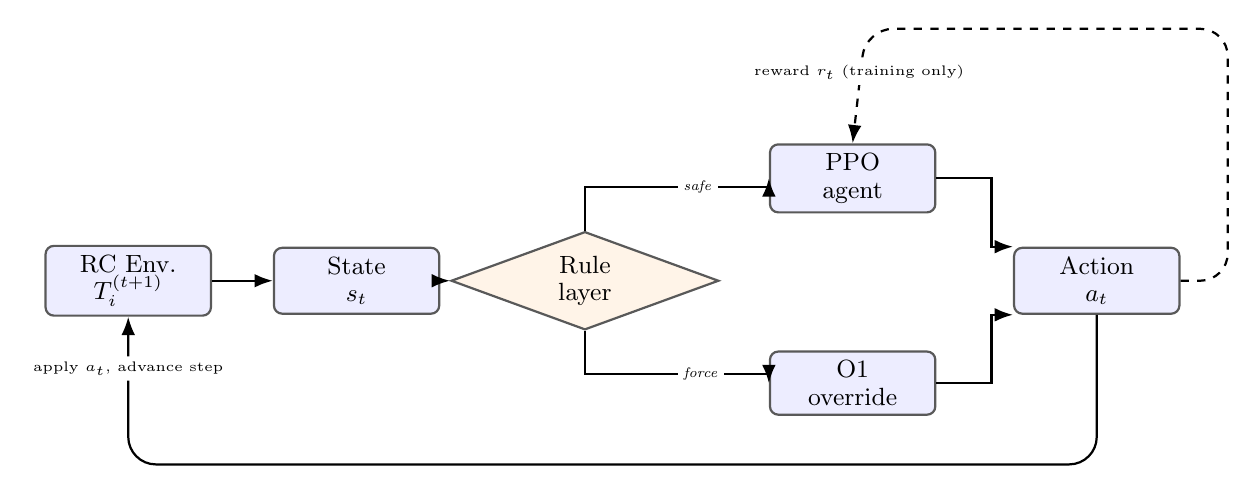
\begin{tikzpicture}[
  box/.style={rectangle,draw=black!65,rounded corners=3pt,thick,
              minimum width=2.1cm,minimum height=0.76cm,
              align=center,fill=blue!7,font=\small},
  dec/.style={diamond,draw=black!65,thick,aspect=2.4,
              fill=orange!9,align=center,font=\small,
              minimum width=3.4cm,minimum height=0.72cm},
  arr/.style={-Latex,thick},
  note/.style={font=\tiny,inner sep=2pt,fill=white,draw=none}]
%%
%% Nodes
\node[box](env)   at ( 0.0,  0  ) {RC Env.\\[-1pt]$T_i^{(t+1)}$};
\node[box](state) at ( 2.9,  0  ) {State\\[-1pt]$s_t$};
\node[dec](rule)  at ( 5.8,  0  ) {Rule\\[-1pt]layer};
\node[box](rl)    at ( 9.2,  1.3) {PPO\\[-1pt]agent};
\node[box](ovr)   at ( 9.2, -1.3) {O1\\[-1pt]override};
\node[box](act)   at (12.3,  0  ) {Action\\[-1pt]$a_t$};
%%
%% Main pipeline: env → state → rule
\draw[arr](env) -- (state);
\draw[arr](state) -- (rule);
%%
%% Branch from rule.north → PPO (safe path, above)
\draw[arr](rule.north) -- ++(0,0.55) -| node[note,right,pos=0.25]{\textit{safe}} (rl.west);
%%
%% Branch from rule.south → override (force path, below)
\draw[arr](rule.south) -- ++(0,-0.55) -| node[note,right,pos=0.25]{\textit{force}} (ovr.west);
%%
%% PPO → action (upper path)
\draw[arr](rl.east) -- ++(0.7,0) |- (act.north west);
%%
%% Override → action (lower path)
\draw[arr](ovr.east) -- ++(0.7,0) |- (act.south west);
%%
%% Smooth feedback loop: action → env (routed below override)
\draw[arr,rounded corners=10pt] (act.south)
  -- ++(0,-1.9)                 % go below the diagram
  -- ++(-12.3,0)                % move left under all boxes
  -- ++(0,0.9)                  % go up toward env
  -- (env.south)
  node[note,below,midway]{apply $a_t$, advance step};
%%
%%
%% Smooth reward loop: action → PPO (dashed)
\draw[arr,dashed,rounded corners=10pt] (act.east)
  -- ++(0.6,0)                % move right of Action
  -- ++(0,3.2)                % go vertically above PPO
  -- ++(-4.6,0)               % move left toward PPO
  -- (rl.north)               % connect from above
  node[note,above,midway]{reward $r_t$ (training only)};
\end{tikzpicture}}% end resizebox
\caption{RBRL architecture.
The \emph{rule layer} branches along two paths: (i)~the \emph{safe} path
routes to the PPO agent when no comfort boundary is threatened; (ii)~the
\emph{force} path overrides the agent with the O1-enforcing action when a
boundary is imminent.
The PPO agent minimises the limit-average cost via reward $r_t$ during
training; the dashed reward loop is inactive at deployment.}
\label{fig:framework}
\end{figure*}
 
\subsection{State Space}
\label{subsec:state}
 
At interval $t$ the agent observes:
\begin{equation}
\begin{split}
  s_t=\Bigl(&
    \underbrace{T_i^{(t)}}_{i\in\mathcal{N}},\;
    \underbrace{\Tiz{i}^{(t)}}_{i\in\mathcal{N}},\;
    \underbrace{\Tout^{(t:t+3)}}_{\text{forecast}},\\
  &\;\underbrace{h_t}_{\text{hour}},\;
    \underbrace{u_i^{(t-1)}}_{i\in\mathcal{N}},\;
    E_{\mathrm{cum}}^{(t)}
  \Bigr)\in\Rset^{3N_z+5}.
\end{split}
  \label{eq:state}
\end{equation}
Two of these state variables do work the others do not~\cite{Li2024MZ}.
\emph{Effective inter-zone temperature} $\Tiz{i}^{(t)}$ (equation~\eqref{eq:tiz}): without this the agent cannot anticipate inter-zone heat loading and inadvertently schedules zones in ways that trigger Rule~R1 in neighbours on the next interval.
\emph{Cumulative energy} $E_{\mathrm{cum}}^{(t)}$: under Model~S the per-step cost \emph{rate} depends on it (the feature that removes the problem from the SLHA class, Section~\ref{subsec:slha}), so the state must carry it. By Proposition~\ref{prop:path} it does not encode an exploitable timing incentive.
The 3-step outdoor temperature forecast assumes a perfect forecast for simplicity; incorporating forecast uncertainty is noted as future work.
 
\subsection{Rules and Action Space}
\label{subsec:rules}
 
\begin{definition}[Rule-based overrides]
\label{def:rules}
\begin{align}
  &\textbf{R1}\;(\text{hard, force on:})\;
    T_i^{(t)}\ge\Tmax-\epsilon_{\mathrm{hot}}
    \;\Rightarrow\;u_i^{(t)}\leftarrow1. \label{eq:R1}\\
  &\textbf{R2}\;(\text{hard, force off:})\;
    T_i^{(t)}\le\Tmin+\epsilon_{\mathrm{cold}}
    \;\Rightarrow\;u_i^{(t)}\leftarrow0. \label{eq:R2}
\end{align}
\end{definition}

The guard bands are \emph{asymmetric} and are derived, not assumed. Each
must absorb the temperature excursion of one actuation interval in its own
direction:
\begin{equation}
\begin{aligned}
  \epsilon_{\mathrm{cold}}&\ge\frac{\Qhvac\Delta t}{\Cth},\\
  \epsilon_{\mathrm{hot}}&\ge\frac{\Delta t}{\Cth}\max_t\!\left[\Lambda_i(\Tout^{(t)}{-}\Tmax)+Q_{\mathrm{sol}}^{(i,t)}\right].
\end{aligned}
  \label{eq:guard}
\end{equation}
The two differ because cooling is driven by the plant and warming by the load.
At the parameters of Table~\ref{tab:params} the cooling excursion is
$0.375\,^\circ$C; the peak seasonal load of $690$, $664$ and $513\,$W across the
three cities gives warming excursions of $0.129$, $0.125$ and
$0.096\,^\circ$C. Cooling is about $2.9$ times the fastest warming, so
$\epsilon_{\mathrm{cold}}=0.40$ and $\epsilon_{\mathrm{hot}}=0.20\,^\circ$C are
adopted. A single symmetric $\epsilon_{\mathrm{g}}=0.5\,^\circ$C, as used
previously, is both unsafe on the cold side at larger intervals and needlessly
restrictive on the hot side: on a $2\,^\circ$C band it would confine the agent to
$(22.5,23.5)$, which excludes TUNED's own switch points $(23.60,22.35)$, so the
rule layer would forbid the best rule in the agent's own family.
Equation~\eqref{eq:guard} instead permits $(22.40,23.80)$; both bands are
drawn to scale in the repository (Section~\ref{sec:data}).

Rule R3, a soft bias toward pre-cooling, is \textbf{withdrawn}, and
Proposition~\ref{prop:path} closes the question more firmly than the earlier
justification did. It is not merely that pre-cooling fails to pay under a
\emph{constant} marginal price; it fails under every cost model used here,
because the bill depends on total consumption alone while pre-cooling raises
that total (Remark~\ref{rem:energy_identity}). The $3.5\%$ contribution
previously claimed for R3 is in any case not reproducible. The condition under
which pre-cooling would become rational is worth stating, since it is a
physical one, not a tariff one: shifting cooling from $t_2$ back to
$t_1$ pays only if the price of \emph{delivered} cooling falls by more than the
store leaks over the interval, which at $\tau=\Cth/\Lambda_i=56.1\,$h is
$3.5\%$ over a four-hour shift and $6.8\%$ over eight, averaged over the
shift; the end-point figures $1-e^{-\Delta t/\tau}$ are $6.9\%$ and
$13.3\%$. A cumulative-block tariff
supplies none of that. A temperature-dependent coefficient of performance would
supply $15$--$20\%$ across a typical diurnal swing and is the route by which a
pre-cooling rule could be reinstated, which is why
Section~\ref{subsec:limits} names the constant-COP assumption as the one most
likely to understate what a scheduler could achieve. R1 and R2 alone enforce
O1, by construction, not by training.
The action is $a_t=(u_1^{(t)},\ldots,u_{N_z}^{(t)})\in\{0,1\}^{N_z}$.
A single shared PPO head is used; the architecture generalises to several zones by factoring the policy head~\cite{Yu2021}, which is not exercised here.
 
\subsection{Reward Function and PPO Architecture}
\label{subsec:reward}
 
The per-step reward augments the negative cost with a quadratic comfort penalty (see equation~\eqref{eq:reward}; at deployment the penalty is zero whenever the hard rules hold the sampled state inside the band):
\begin{equation}
\begin{split}
  r_t=-\sum_{i\in\mathcal{N}}c_i^{(t)}
  -\alpha\sum_{i\in\mathcal{N}}\Bigl[&\max\!\bigl(0,T_i^{(t)}-\Tmax\bigr)^2\\
  &+\max\!\bigl(0,\Tmin-T_i^{(t)}\bigr)^2\Bigr],
\end{split}
  \label{eq:reward}
\end{equation}
with $\alpha=50$. The quadratic comfort penalty drives the agent away from boundaries during training; it is identically zero at deployment.
The shared policy network maps $s_t$ via two fully connected layers (256--128 units, ReLU) to per-zone Bernoulli probabilities, plus a value head.
PPO clip coefficient: $\epsilon_{\mathrm{clip}}=0.2$.
Training runs for $2\times10^{5}$ environment \emph{steps} (about $298$
episodes of $672$ steps, one $168\,$h window at $\Delta t=15\,$min) each
episode drawing its start date from the six tuning windows of
Section~\ref{sec:sim}, which are disjoint from the seven evaluation windows. The
earlier version reported $2\times10^{5}$ \emph{episodes} ($3.36\times10^{7}$
steps) and a convergence episode; both belonged to the withdrawn pipeline and
are corrected, not carried over. No convergence claim is made: under the
hard rule layer the attained cost does not depend on how long the agent trains,
because the rules alone determine it (Corollary~\ref{cor:rules_sufficient}), and
nine of ten Riyadh and Jeddah seeds reach the rule's own trajectory exactly
(Table~\ref{tab:abl_component}).
Algorithm~\ref{alg:rbrl} sets out training and schedule extraction together; the
policy $\pi_\theta$ it returns is the one evaluated in every RBRL row of
Section~\ref{sec:results}.
 
\begin{algorithm}[H]
\caption{RBRL: Training and Schedule Extraction}
\label{alg:rbrl}
\begin{algorithmic}[1]
\Require RC simulation, weather profile $\mathcal{W}$, cost model $m$,
  episode length $N_{\mathrm{tr}}=672$ intervals ($168\,$h at
  $\Delta t=15\,$min), evaluation length $N_{\mathrm{ev}}=672$,
  switching cost $\csw$, total budget $B=2\times10^{5}$ environment steps,
  occupied ceiling $\overline{T}$ (Section~\ref{subsec:protocol})
\Ensure Safe schedule $\sched^*$
\Statex \textbf{Phase 1: training}
\State Initialise PPO policy $\pi_\theta$ randomly; $n\leftarrow0$
\While{$n<B$} \Comment{fixed budget; no early stopping}
  \State Sample start date $d_0\sim\mathcal{W}$ (tuning split only);
         reset $T_i^{(0)}\!=\!23\,^\circ$C, $E_{\mathrm{cum}}\!\leftarrow\!E_{\mathrm{base}}$
  \For{$t=0$ \textbf{to} $N_{\mathrm{tr}}-1$}
    \State Observe $s_t$ via~\eqref{eq:state}
    \State $a_t\sim\pi_\theta(\cdot\,|\,s_t)$ \Comment{stochastic during training}
    \For{each zone $i$}
      \State $u_i^{(t)}\leftarrow a_{t,i}$ \Comment{interior: the agent decides}
      \If{$T_i^{(t)}\ge\overline{T}-\epsilon_{\mathrm{hot}}$}
        $u_i^{(t)}\leftarrow1$ \Comment{R1, enforces O1}
      \ElsIf{$T_i^{(t)}\le\Tmin+\epsilon_{\mathrm{cold}}$}
        $u_i^{(t)}\leftarrow0$ \Comment{R2, enforces O1}
      \EndIf
    \EndFor
    \State Step~\eqref{eq:rc_disc}; accumulate $E_{\mathrm{cum}}$;
           compute $c_i^{(t)}$ and $r_t$~\eqref{eq:reward}; $n\leftarrow n+1$
  \EndFor
  \State Update $\pi_\theta$ by PPO (clipped surrogate, GAE)
\EndWhile
\State\Return the final $\pi_\theta$ \Comment{no checkpoint selection}
\Statex \textbf{Phase 2: schedule extraction}
\State Reset on a held-out start date; $E_{\mathrm{cum}}\leftarrow E_{\mathrm{base}}$
\For{$t=0$ \textbf{to} $N_{\mathrm{ev}}-1$}
  \State $a_t\leftarrow\arg\max_a\pi_\theta(a\,|\,s_t)$ \Comment{deterministic}
  \State Apply R1--R2 as above; step~\eqref{eq:rc_disc}
\EndFor
\State\Return $\sched^*=\{u^{(t)}\}_{t=0}^{N_{\mathrm{ev}}-1}$
\end{algorithmic}
\end{algorithm}
 
\subsection{Competing Methods}
\label{subsec:compete}
 
\textbf{THERM (unoptimised baseline)} models the automatic remote-controller thermostat used across Saudi residential buildings~\cite{Alotaibi2024}: on when $T_i\ge\Tmax-0.5$, off when $T_i\le\Tmin+0.5$, with no tariff awareness.
On the occupied band adopted here this is a $1\,^\circ$C deadband centred on
$23\,^\circ$C, which is simultaneously the definition above and a representative
hardware deadband for the split units in this stock. The distinction matters for
how the results should be read: the advantage every optimising controller holds
over THERM comes from being free to use the whole $2\,^\circ$C comfort band
where THERM uses only $1\,^\circ$C of it, so the comparison is between a
fixed-deadband device and a scheduler with the same comfort obligation, not
between two controllers with different comfort obligations.

\textbf{TUNED (rule-based comparator)} is the same hysteresis family with its two
switch points free, chosen by exhaustive search over a $0.05\,^\circ$C grid.
Including it is essential: without it, any gap attributed to learning may in fact
be obtainable by commissioning the thermostat properly. It is tuned on one set
of evaluation windows and reported on a disjoint set
(Section~\ref{subsec:protocol}).

\textbf{CLV (clairvoyant optimality reference)} is a dynamic programme over the
exact dynamics~\eqref{eq:rc_disc} on a $10\,$mK grid, with the terminal thermal
state priced so that no controller is rewarded for ending the horizon warm. It
sees the entire weather trajectory in advance. It is reported as a
\emph{bracket}, not a single number, because a clairvoyant programme
constrained to match comfort does not by itself bound a causal controller
unless the two are held to the same comfort requirement; Section~\ref{subsec:bound}
derives the bracket and explains why the obvious construction, a constant
occupied ceiling, is not a bound at all. The lower end is a schedule that is
attainable; the upper end is a Lagrangian limit no mean-matched schedule can
beat. The gap between TUNED and that bracket is the headroom a learned policy
could in principle occupy.

\textbf{MPC (causal receding-horizon comparator)} solves the same Bellman
recursion over a finite lookahead at every interval, applies the first action
and re-solves. It has the same plant, band, tariff and switching cost as the
other arms, and a perfect forecast \emph{only} inside its horizon; beyond it
the weather is unknown. It is the term that separates two otherwise confounded
explanations of this paper's negative result---that there is nothing to gain
inside the rule-constrained class, and that what there is to gain requires a
forecast the agent does not have. Horizons of $6$ and $24\,$h are reported in
Section~\ref{subsec:abl_component}.

The genetic-algorithm and simulated-annealing comparators of the earlier
version of this study~\cite{ElMakroum2023,Bandarra2025} are \textbf{withdrawn}.
Both are day-ahead offline solvers, and a metaheuristic's cost is evidence only
about that metaheuristic's convergence; the Lagrangian bound
of~\eqref{eq:dual_bound} applies to them as to every other mean-matched
schedule, so it answers the question they were introduced to answer and removes
the need to argue about their tuning. No third-party learned comparator (SAC,
DQN) is run, for the stronger form of the same reason: the clairvoyant
programme solved over exactly the rule-admissible action set
(Remark~\ref{rem:cor_scope}) upper-bounds \emph{every} policy in the class any
such learner would occupy, at $6.3\%$ against the hysteresis's $5.8\%$, and
the Lagrangian limit bounds every mean-matched schedule outside it. An
empirical run of one more learner would be strictly weaker evidence than the
bound already reported, since a learner's shortfall is evidence about its
training, not about the class.
 
The framework is applied to the three climates characterised next.
 
%% ============================================================
\section{Case Studies: Riyadh, Jeddah and Taif}
\label{sec:casestudy}

Three sites are used, chosen to span the conditions under which a Saudi dwelling
is cooled, not to represent the Kingdom: hot-arid inland (Riyadh),
hot-humid coastal (Jeddah) and mild highland (Taif).
 
\subsection{Climate Profiles}
\label{subsec:climate}
 
Riyadh (BWh, $24.7^\circ$N, $635\,$m) is an inland desert city with summer highs
reaching $46.6\,^\circ$C and a cooling-season diurnal swing of $12.7\,$K, the
largest of the three sites (CDD$_{18}=3{,}693$; cf.~\cite{Haddad2024}).
Jeddah (BSh, $21.7^\circ$N, $15\,$m) is a Red Sea coastal city, classified
hot-humid~\cite{Rodrigues2025}; in the record used here its annual mean
relative humidity is $58.5\%$ with $17.5\%$ of hours above $70\%$, and it has a
compressed diurnal swing of $8.4\,$K and little overnight relief
(CDD$_{18}=4{,}260$). The degree-day
comparison between the two sites is sensitive to the choice of typical-year
record and should not be relied upon: the TMYx record used here places Jeddah
\emph{above} Riyadh, because Jeddah's milder winters raise its annual total
while Riyadh retains the hotter peaks, whereas the older IWEC files reverse the
ordering. What distinguishes the sites for the purposes of this work is not the
annual degree-day total but the diurnal swing, which governs pre-cooling
headroom and is larger in Riyadh under both records.
Taif (BSh, $21.3^\circ$N, $1{,}478\,$m) is a highland site whose altitude lowers
both the peak and the mean: over the cooling season its mean outdoor temperature
is $28.6\,^\circ$C against Riyadh's $35.0$ and Jeddah's $32.7$, and its peak
$39.4\,^\circ$C against $46.6$ and $44.0$, and CDD$_{18}=2{,}277$ against
$3{,}693$ and $4{,}260$. Its diurnal swing, $11.7\,$K, is
close to Riyadh's. The load is therefore the smallest of the three while the
headroom is not, which is why Taif leaves the least to schedule in absolute
terms and shows the largest window-to-window dispersion
(Section~\ref{subsec:consumption}); the lower air density at that altitude is
also why the infiltration conductance is evaluated per city
(Section~\ref{subsec:sbc}).
Monthly and diurnal profiles for the three sites are plotted in the repository
(Section~\ref{sec:data}) directly from the records, not reproduced
here. All three simulations use
TMYx typical-year records from
\texttt{climate.onebuilding.org}, WMO~404380 (Riyadh, period of record
2009--2022, $12$ years), 410240 (Jeddah, 2009--2023, $15$ years) and
410360 (Taif, 2009--2023, $15$ years), in preference to the older IWEC files; hourly dry-bulb temperature
and the direct-normal and diffuse-horizontal irradiances are read from
fields~7, 15 and~16, and the glazing gain is the plane-of-array irradiance on a
south-facing vertical surface under an isotropic sky with ground albedo
$0.30$.
 
 
\subsection{Building Code, Tariff, Humidity, and Comfort Standard}
\label{subsec:sbc}
 
SBC~2018 mandates opaque-wall U-value $\le0.45\,\text{W\,m}^{-2}\text{K}^{-1}$ and window SHGC $\le0.25$ in both Climate Zone~A (Jeddah) and Zone~B (Riyadh)~\cite{Alayed2021}. Table~\ref{tab:params} meets both at assembly level: $U_{\mathrm{wall}}=0.45$ and $\mathrm{SHGC}=0.25$ exactly, with $U_{\mathrm{win}}=2.8\,\text{W\,m}^{-2}\text{K}^{-1}$ consistent with the double glazing described in the text. This corrects the earlier version's envelope ($\lext=25.0$ and $\lwin=8.0\,\mathrm{W/K}$: transmittances of $1.79$ and $4.00\,\text{W\,m}^{-2}\text{K}^{-1}$, both above the prescriptive maxima), whose excess load biased any percentage saving optimistically; the compliant envelope removes that bias in the conservative direction.
The multi-tier step-wise tariff follows equation~\eqref{eq:stepwise}; for Models~L and~E, $c_r^{\mathrm{L}}=0.12\,\SAR/\kWh$ is adopted as a mid-range flat rate, comparable to the post-2018 first-block price. It is \emph{not} the consumption-weighted average of~\eqref{eq:stepwise} over this account, which at ${\approx}884\,\kWh$ is the first-block rate of $0.05\,\SAR/\kWh$ exactly; the consequences of this choice for the cost-model ablation are taken up in Section~\ref{subsec:disc_modele}.
The occupied comfort band $[22,24]\,^\circ$C is consistent with the \emph{thermal} criterion of ASHRAE~55-2023~\cite{ASHRAE55_2023} for mechanically conditioned residential spaces (the standard's humidity criterion is not evaluated here, and Section~\ref{subsec:disc_limits} reports where it would bind), as validated by Bienvenido-Huertas et al.~\cite{Bienvenido2024}, and its upper limit reflects Saudi practice as discussed in Section~\ref{subsec:thermal}: Krarti~\cite{Krarti2020occ} recommends $23$--$25\,^\circ$C for Kingdom dwellings and observes setpoints as low as $18\,^\circ$C in the stock.
Lamsal et al.~\cite{Lamsal2023} review adaptive thermal comfort models and find wider deadbands appropriate for energy-efficient design in hot climates; the narrower band adopted here is therefore conservative with respect to that literature, and the band width is reported as a sensitivity, not assumed, because it is the single parameter to which the reported saving is most sensitive (Section~\ref{subsec:disc_band}).
A fixed band is adopted because Saudi residential buildings are predominantly mechanically cooled; ASHRAE~55 Section~5.3 restricts adaptive comfort to naturally ventilated spaces.
The framework accommodates narrower or wider bands by adjusting $\Tmin/\Tmax$, but the saving does not transfer across band widths: the actuation condition~\eqref{eq:deadband_condition} and the baseline's cycling rate both depend on the width, so a band change requires re-evaluation, not re-scaling.
 
\emph{Humidity and latent heat.}
The RC model captures sensible heat only. The sensible heat ratio is not taken
from the literature but computed from the humidity fields of the records used
here: over the cooling season the infiltration SHR is $0.98$ in Riyadh, $0.79$
in Taif and $0.32$ in Jeddah, so the coastal site is majority \emph{latent}
while the inland one is almost purely sensible. To measure what this
idealisation costs, the study is re-run on a two-state zone model built on the
\emph{same} parameters, solar transposition and matching protocol as the main
model (its sensible-only arm reproduces the main results to machine
precision) extended by a moisture balance with hygric buffering, an SHR-limited
coil whose latent removal is driven by the zone state against the apparatus dew
point, and a saturation clamp that condenses excess moisture and returns the
enthalpy of vaporisation to the sensible node, so relative humidity cannot
exceed $100\%$ by construction. (The earlier version of this side study applied
\emph{horizontal} irradiance to the vertical glazing, omitted comfort matching
and allowed $103.8\%$ relative humidity; its deltas are superseded by the
figures here, which reverse its sign in Jeddah.) Latent load raises the
baseline's delivered energy by $33.9\%$ in Jeddah, $2.3\%$ in Taif and $0.7\%$
in Riyadh. The effect on the reported saving differs by city in both size and
sign, re-tuned and re-matched within each physics variant: $+0.4$ points in
Riyadh; $+3.7$ points in Jeddah, where latent load consumes coil capacity
($20\%$ of runtime at the rated latent limit), lengthens on-phases, and makes
the longer cycles of the tuned rule worth more; and $-4.6$ points in Taif,
where under latent physics no rule in the family is both comfort-matched and
cheaper than the baseline, so the tuned rule collapses onto it. The sensible-only
headline is therefore conservative for Jeddah and optimistic for Taif. The
comfort caveat is sharper than the cost one: at rated $\mathrm{SHR}=0.75$ the
Jeddah zone exceeds the ASHRAE~55-2023 humidity-ratio limit of
$0.012\,$kg/kg for $85\%$ of occupied time (outdoor air exceeds it $99\%$ of
the time), so in the humid coastal climate \emph{no} controller in this
action space maintains latent comfort with this plant, and the comparison
there is cost at matched dry-bulb comfort only. The claim made in the earlier
version of this study, that the penalty cancels because every arm carries
it, does not hold as reasoning: a multiplicative error on the energy term does
not cancel in a ratio whose numerator is an additive switching term, and the
sign of its effect differs by city.
 
%% ============================================================
\section{Simulation Setup}
\label{sec:sim}
 
All simulations run in Python~3.11 with a custom RC environment integrating
equation~\eqref{eq:rc_disc} at $\Delta t=15\,\text{min}$, the interval adopted
throughout and the one that satisfies~\eqref{eq:deadband_condition} with a
factor of $2.7$ margin; the hourly interval of the earlier version does not
(Remark~\ref{rem:rc}). No claim is made about the hardware on which they were
executed; see Section~\ref{subsec:abl_cost}.

\paragraph{Non-HVAC background load and tariff activation}
Because the Saudi tariff is levied on the whole customer account, not on
the HVAC circuit alone, the cumulative-energy state $E_{\mathrm{cum}}$ is
initialised with a non-HVAC household base load of
$E_{\mathrm{base}}\approx800\,\kWh$/month (lighting, appliances and water
heating), consistent with the residential end-use breakdown reported for Saudi
dwellings by Al-Homoud and Krarti~\cite{AlHomoud2021}. Whether the step-wise structure is exercised at all follows from the
arithmetic, and for the configuration actually evaluated here it is not. The
single zone consumes $2.80\,\kWh$/day, or ${\approx}84\,\kWh$ over a 30-day
billing month, so with the base load the account reaches
${\approx}884\,\kWh$ and crosses no boundary of any schedule. A multi-zone
dwelling of the class the formulation covers would: sixteen such zones would
place the account near the first boundary of the historical four-tier schedule
($2{,}000\,\kWh$), which is why Model~S is retained in the formulation as a
stress test, not a representation of this account. The same arithmetic shows why
the tariff now in force behaves differently: its only boundary sits at
$6{,}000\,\kWh$, which this account does not approach, so no traversal occurs
(Remark~\ref{rem:current_tariff}).
Training hardware and wall-clock training time are not reported, for the reason given in Section~\ref{subsec:abl_cost}.
Training uses five independent random seeds $\{42,\dots,46\}$; for each seed the trained policy is evaluated on the seven held-out windows of Section~\ref{subsec:protocol}, and every reported figure is the mean $\pm$\,std over \emph{all} five seeds. No seed is discarded and no best-of-$n$ selection is applied, so the reported spread is the true run-to-run variability, not a best-case estimate. Training proceeds for a \emph{fixed} budget with no early stopping and no intermediate checkpoint selection: the policy evaluated is the final one. This matters because the saving is non-monotone during training; a best-checkpoint rule scored on the test weeks would select partly on test noise and bias every reported figure upward.

Solar gain is $Q_{\mathrm{sol}}^{(i,t)}=\text{SHGC}\times A_{gl}\times I^{(t)}$, with $I^{(t)}$ the plane-of-array irradiance on a south-facing vertical surface, computed from the EPW direct-normal and diffuse-horizontal fields under an isotropic sky with ground albedo $0.30$ as set out in Section~\ref{subsec:climate}~\cite{EPW2023}.

\paragraph{Evaluation protocol.}
\label{subsec:protocol}
The weather record is a single typical-meteorological EPW year of $8{,}760\,$h
per city~\cite{EPW2023}, so the split is made \emph{within} that year, by
calendar date, and is stated here in full.

Evaluation is confined to the cooling season, 1~May to 31~October. The plant is
cooling-only and cannot hold $\Tmin$ in the shoulder months, so a figure
averaged over a full year would combine a control result with months in which no
control is exercised; the earlier version of this study reported ``zero comfort
violations across all configurations and seasons'', and that claim is withdrawn
and replaced by one restricted to the evaluated season.

Thirteen windows of $168\,$h are laid down at $14$-day intervals from
day-of-year $121$ to $289$. They are assigned alternately: the six odd-indexed
windows form the \emph{tuning} set and the seven even-indexed windows the
\emph{held-out} set. The two switch points of TUNED are chosen to minimise mean
cost over the tuning windows, subject to zero occupied degree-hours and to the
comfort match in \emph{every} one of them, and are then applied unchanged to the
held-out windows. No held-out window contributes to the choice of any
\emph{control} parameter: TUNED's two switch points are fitted on the tuning
windows alone, and the PPO policy is trained on episodes drawn only from them.
One parameter is an exception and must be declared, because it is not a control
parameter but the device that makes the arms comparable. The occupied ceiling
used to match each arm's mean temperature to the baseline's is searched on the
\emph{held-out} windows, since it is on those windows that the match has to
hold. For the clairvoyant and receding-horizon arms that is a normalisation and
nothing else. For RBRL it is not neutral: the rule layer forces the compressor
on at $\mathrm{cap}-\epsilon_{\mathrm{hot}}$, so moving the ceiling moves R1's
own threshold. RBRL and the guard hysteresis therefore have one parameter
fitted where they are scored, while TUNED has none, and the comparison between
them is asymmetric in RBRL's favour by that much.
Section~\ref{subsec:abl_component} returns to this where it matters most.
Because the windows are spaced by $14$ days and are $7$ days long,
none overlaps any other, which the earlier version's protocol could not achieve.

Dispersion is reported as the standard deviation of the \emph{paired}
per-window saving, each window serving as its own baseline. Pairing is necessary
rather than decorative here: THERM's daily cost ranges from $0.72$ to
$1.35\,\SAR$/zone across the Riyadh windows, a factor of $1.9$, so an unpaired
standard deviation would be dominated by seasonal load variation, not by
controller performance.
The PPO agent uses Stable-Baselines3~\cite{Raffin2021} (v2.9.2) on
Gymnasium; the simulator, the clairvoyant dynamic programme and the tuned rule
are implemented directly in NumPy~(v2.5.3).
All costs are reported per 24\,h: $\Jbar$ of~\eqref{eq:cop} is a per-interval
mean, multiplied by $24/\Delta t$ before tabulation. Four metrics are reported:
daily cost per zone, daily energy per zone, switching frequency, and comfort as
\emph{occupied degree-hours} outside the band, not as a violation rate,
because a count fraction carries neither the magnitude nor the cause of an
excursion, and cause decides standing. An excursion is a \emph{control failure} if the plant was commanded on
over the interval, or if it was off while the outdoor air was inside or above
the band: in either case an admissible alternative action would have avoided
it. It is a \emph{plant limit} only when the zone free-floats below the band
with the compressor off and the outdoor air below it, where a cooling-only
plant cannot respond; sign alone would misclassify in both directions. The
configurations this paper calls inadmissible (an hourly interval,
$\Cth\le1{,}800\,$kJ/K, a $1.5\,^\circ$C deadband) all fail through
under-temperature arising while the compressor is \emph{on}, as
$\Qhvac\Delta t/\Cth$ overshoot ($15.44\,^\circ$C$\cdot$h of commanded-on
undershoot against $2.53$ of free-float on the Riyadh window of
Table~\ref{tab:timestep}), whereas the Taif baseline's
$0.156\,^\circ$C$\cdot$h carries no commanded-on component. For a single zone
the degree-hour measure is exact on the actuation grid, the trajectory being
monotone between actuations.
Key PPO hyperparameters are listed in Table~\ref{tab:ppo}; the RC model assumes no occupancy heat gains. The switch-on cost $\csw=0.15\,\SAR$ amortises compressor start-up wear: for a split unit of ${\sim}2{,}500\,\SAR$ installed cost, a start life on the order of $10^{5}$ gives $0.025\,\SAR$ per start, while a ${\sim}15$-year design life at the ${\sim}4$ starts per day measured here gives ${\sim}2.2\times10^{4}$ starts and $0.114\,\SAR$. The adopted $0.15\,\SAR$ lies \emph{above} both figures this reasoning
supports, which must be stated plainly rather than called conservative: the
percentage grows monotonically in $\csw$, since the saving is realised through
a reduction in activations. At the two values the derivation does support
the Riyadh headline falls from $9.3\%$ to approximately $7.7\%$ at
$\csw=0.114$ and to approximately $2.5\%$ at $\csw=0.025$, and at $\csw=0$ it
is $0.1\%$ (Table~\ref{tab:sensitivity}(b)). No external measurement of
per-start wear cost for Saudi residential split units is cited here because
none was found: a search of manufacturer application literature, the AHRI and
ASHRAE sources on cycling (which quantify the \emph{part-load efficiency}
penalty of cycling, not a per-start cost), and the LBNL short-cycling studies
of DX equipment~\cite{Pang2011} returned no quantified cost or life
consumption per start. Until one exists, the cost figures in this paper should
be read as a scaling of the start reduction, which is the quantity actually
measured, and not as an independent result. The ranking of controllers is
unchanged across the range (Table~\ref{tab:sensitivity}(b)).
The numerical study evaluates the single zone only; Section~\ref{subsec:limits} sets out why, and why a multi-zone instance is the setting in which Corollary~\ref{cor:rules_sufficient}'s hypotheses fail and a learned policy would have something to contribute.
 
\begin{table}[htbp]
\setlength{\hfuzz}{6pt}
\caption{PPO training hyperparameters, as used for the results reported here.
Values not listed are the Stable-Baselines3 v2.9.2 defaults.}
\label{tab:ppo}
\centering

\begin{subtable}{\columnwidth}
\setlength{\tabcolsep}{5pt}
\begin{tabularx}{\columnwidth}{@{}>{\raggedright\arraybackslash}X X@{}}
\toprule
\textbf{Parameter} & \textbf{Value} \\
\midrule
Network (FC)                 & 256--128 units, ReLU, actor and critic \\
Learning rate                & $3\times10^{-4}$ (Adam, constant) \\
Discount $\gamma$ / Clip $\varepsilon$ & $0.999$\,/\,$0.2$ \\
Entropy coefficient          & $0$ (no exploration bonus) \\
Rollout $n_{\mathrm{steps}}$ / batch & $1{,}344$\,/\,$336$ \\
Training budget              & $2\times10^{5}$ environment \emph{steps} \\
Episode length               & $672$ steps ($168\,$h at $\Delta t=15\,$min) \\
Seeds                        & $5$ ($42$--$46$), none discarded \\
\bottomrule
\end{tabularx}
\end{subtable}
 
\end{table}
 
Hyperparameters are listed in Table~\ref{tab:ppo} as used; every value not
listed is the Stable-Baselines3~\cite{Raffin2021} default for the version
stated. No hyperparameter search was performed for the results reported here
(the grid search described in the earlier version ran on a withdrawn pipeline),
and Corollary~\ref{cor:rules_sufficient} explains why this costs little: under
the hard rules at matched comfort the attainable cost does not depend on the
learned policy, a prediction the ablation confirms
(Table~\ref{tab:abl_component}). The seed dispersion is itself a finding, and
Section~\ref{subsec:abl_component} quantifies it.
 

 
%% ============================================================
\section{Results}
\label{sec:results}
 
Results are reported over the cooling season, 1~May to 31~October, on the
held-out windows of Section~\ref{subsec:protocol}, with comfort as occupied
degree-hours outside the band (taxonomy by cause in
Section~\ref{sec:sim}); every arm records $0.000\,^\circ$C$\cdot$h of
\emph{over}-temperature. Two exceptions are reported, not suppressed: the
no-rules ablation row of Table~\ref{tab:abl_component}
($0.085\,^\circ$C$\cdot$h, the point of that row---it is what the rules
prevent), and the $16$~October Taif window, where the outdoor minimum of
$16\,^\circ$C drifts every arm \emph{below} the band (baseline
$0.156\,^\circ$C$\cdot$h, guard-constrained rule $0.350$), a plant limit no
cooling-only controller can correct; the inadmissible configurations of
Table~\ref{tab:timestep} exhibit the actuation condition's failure mode and
are labelled as such.
 
\subsection{What Clairvoyance Is Worth: a Bound and an Attainable Schedule}
\label{subsec:bound}

A clairvoyant reference is only useful if it bounds what a causal controller
could do. The earlier version's device, a dynamic programme forbidden to
exceed a \emph{constant} occupied ceiling, does not: a constant ceiling is a
pointwise restriction where the comparison requires only a matched \emph{mean},
so the capped programme optimises over a strictly smaller set than the
controllers it is meant to bound, and arms matched by other means beat it (the
receding-horizon controller does in Riyadh and Jeddah; in Taif so does the
guard hysteresis).

The constraint that belongs here keeps the band pointwise, because that is the
comfort requirement, and applies the match only in the mean:
\begin{equation}
\begin{split}
  \min_{u}\;&J(u)\quad\text{s.t.}\quad
    T_i^{(t)}\in[\Tmin,\Tmax]\ \ \forall\,t\in\mathcal{O},\\
  &\tfrac{1}{|\mathcal{O}|}\textstyle\sum_{t\in\mathcal{O}}T_i^{(t)}
    \;\le\;T^{\star},
\end{split}
\label{eq:meanconstrained}
\end{equation}
with $\mathcal{O}$ the occupied steps and $T^{\star}$ the baseline's mean. The
constraint is written as an inequality, not an equality, for two reasons.
It is the requirement that actually matters (an arm may not be \emph{warmer}
than the baseline, since only warmth can buy a saving), and with binary actions
on a $15\,$min grid the attainable means form a finite set, so an equality
would generically describe an empty feasible region. Writing it this way also
makes $\lambda\ge0$ a consequence, not an assumption.
Relaxing the mean constraint alone gives
$L(u,\lambda)=J(u)+\lambda\bigl(|\mathcal{O}|^{-1}\sum_{t}T_i^{(t)}-T^{\star}\bigr)$,
which for fixed $\lambda$ is the same dynamic programme with one additional
additive stage cost. For \emph{any} $\lambda$ and any $u$ feasible
for~\eqref{eq:meanconstrained},
\begin{equation}
  J(u)\;=\;L(u,\lambda)\;\ge\;\min_{u'}L(u',\lambda)\;=\;L^{\star}(\lambda),
  \label{eq:dual_bound}
\end{equation}
so $\max_{\lambda}L^{\star}(\lambda)$ lower-bounds the cost of every
mean-matched schedule and hence upper-bounds the saving any of them can
achieve. This holds whether or not the dual gap closes, which matters because
here it does not: the attained mean is a \emph{step} function of $\lambda$. On
the first Riyadh window it sits at $22.991\,^\circ$C for every
$\lambda\in[1.0,1.9]$ and jumps to $22.894$ at $\lambda=2.0$, with the target
$22.941$ in the gap: the binary action set makes the inner minimiser flip
discretely, so no exactly mean-matched schedule need exist in this family.
That is why the earlier attempt to match by bisection could not succeed, and
why a pointwise cap was reached for instead.

Two practical points govern how the bound is computed and how far it should be
trusted. First, $\lambda$ is maximised over $[0,24]$ on an eighteen-point grid
with ten golden-section refinements, giving
$\lambda^{\star}=2.02$, $2.18$ and $1.46$ in Riyadh, Jeddah and Taif.
$L^{\star}(\lambda)$ is a pointwise minimum of functions affine in $\lambda$ and
is therefore concave whatever the action set, so the refinement is sound; and
because~\eqref{eq:dual_bound} holds for \emph{every} $\lambda$, an
under-maximised $\lambda$ weakens the bound without invalidating it. Second,
the inner minimisation is solved on a discrete temperature grid, and a
discretised dynamic programme returns a minimum that is too \emph{expensive},
which makes the saving bound too tight, the unsafe direction. Re-evaluating
$L^{\star}(\lambda^{\star})$ at $1{,}601$, $3{,}201$ and $6{,}401$ points gives
$18.95$, $19.35$ and $19.56\%$ in Riyadh and is still drifting upward at the
finest grid. The bound is therefore quoted at the finest grid plus the last
increment as a margin, rounded outward: $\le19.8$, $\le19.5$ and $\le20.2\%$.
It is rigorous up to that stated discretisation allowance, not beyond it.

Table~\ref{tab:main} therefore reports two clairvoyant quantities instead of
one: the best band-feasible schedule found that is no warmer than the baseline
in \emph{every} window, which is \emph{attainable}, and the
bound~\eqref{eq:dual_bound}. They bracket the optimum; the interval between
them is at most $1.7$ points in Riyadh and Jeddah and $5.2$ in Taif, and every
controller reported in this paper lies below the bound in every city at the
instance evaluated: the tariff in force, $\csw=0.15\,\SAR$,
$\deadband=1\,^\circ$C and $\Delta t=15\,$min. It is not a bound on the
saving available at other deadbands or tariffs, where
Tables~\ref{tab:sensitivity}(a) and~(c) report larger figures against
correspondingly different baselines.

\subsection{Consumption and Cost: Without vs.\ With Optimisation}
\label{subsec:consumption}
 
Three features of Table~\ref{tab:main}'s construction govern how its numbers
should be read. First, every arm is matched to THERM's mean occupied
temperature window by window: the tuned rule to within $0.03\,^\circ$C, and the
clairvoyant arms to within $0.013\,^\circ$C with the residual running
\emph{cool} in every window, so that arm can claim no comfort credit anywhere.
No part of any saving is a deliberate setpoint difference;
Remark~\ref{rem:energy_identity} explains why an unmatched comparison would
largely restate identity~\eqref{eq:duty_identity} instead of comparing
schedules. Second, TUNED is fitted on the six \emph{tuning} windows and reported
on the seven disjoint held-out ones, so the figures are out-of-sample. Third,
dispersion is the paired per-window standard deviation
(Section~\ref{subsec:protocol}).

\begin{table*}[t]
\centering
\caption{Held-out results at the tariff in force ($0.18\,\SAR/\kWh$), occupied
band $[22,24]\,^\circ$C, $\Delta t=15\,$min, single zone with one exposed
face; mean $\pm$ standard deviation of the paired saving over the seven
held-out windows. The saving columns are the mean of the \emph{per-window}
savings, not the saving computed from the mean costs in the $J$ column; the
two differ by up to $0.8$ points in Taif, so dividing the printed costs will
not reproduce the printed percentages. ``CLV'' is the clairvoyant programme of
Section~\ref{subsec:bound}: band-feasible and, in \emph{every} window, no
warmer than that window's own baseline mean (worst drift $-0.013\,^\circ$C),
so it claims no comfort credit and its saving is attainable, a \emph{lower}
estimate of what clairvoyance is worth. The \emph{bound} rows are the
Lagrangian limit~\eqref{eq:dual_bound} under aggregate mean-matching, which no
schedule so matched can beat; the two rows bracket the true optimum, their gap
the duality gap. Energy and start columns are omitted for the clairvoyant
rows, whose matching device differs from the controllers'. Zero
over-temperature degree-hours in every row.}
\label{tab:main}
\setlength{\tabcolsep}{3pt}
\begin{tabularx}{\textwidth}{@{}lXrrr@{}}
\toprule
 & $J$ (SAR/zone/day) & \multicolumn{3}{c}{Saving vs.\ THERM (\%)} \\
\cmidrule(lr){3-5}
Controller & mean $\pm$ sd & Cost & Energy & Starts \\
\midrule
\multicolumn{5}{@{}l}{\textbf{Riyadh}} \\
THERM & $1.1183$ & --- & --- & --- \\
TUNED ($23.60/22.35$) & $1.0170$ & $9.3\pm1.6$ & $-0.3\pm1.0$ & $16.7\pm2.5$ \\
CLV, best schedule found & $0.9174$ & $18.1\pm1.7$ & --- & --- \\
CLV $+$ setback & $0.8310$ & $25.8\pm2.0$ & --- & --- \\
\quad\emph{bound} (\ref{eq:dual_bound}) & $\ge0.8969$ & $\le19.8$ & --- & --- \\
\quad\emph{bound}, $+$ setback & $\ge0.8141$ & $\le27.2$ & --- & --- \\
\midrule
\multicolumn{5}{@{}l}{\textbf{Jeddah}} \\
THERM & $0.9926$ & --- & --- & --- \\
TUNED ($23.60/22.35$) & $0.9006$ & $9.3\pm1.4$ & $0.5\pm1.6$ & $16.4\pm2.5$ \\
CLV, best schedule found & $0.8161$ & $17.8\pm1.9$ & --- & --- \\
CLV $+$ setback & $0.7367$ & $25.8\pm1.2$ & --- & --- \\
\quad\emph{bound} (\ref{eq:dual_bound}) & $\ge0.7990$ & $\le19.5$ & --- & --- \\
\quad\emph{bound}, $+$ setback & $\ge0.7206$ & $\le27.4$ & --- & --- \\
\midrule
\multicolumn{5}{@{}l}{\textbf{Taif}} \\
THERM & $0.6139$ & --- & --- & --- \\
TUNED ($23.60/22.50$) & $0.5881$ & $4.6\pm3.6$ & $-0.1\pm3.1$ & $7.5\pm5.3$ \\
CLV, best schedule found & $0.5170$ & $15.0\pm6.9$ & --- & --- \\
CLV $+$ setback & $0.4761$ & $21.5\pm6.0$ & --- & --- \\
\quad\emph{bound} (\ref{eq:dual_bound}) & $\ge0.4899$ & $\le20.2$ & --- & --- \\
\quad\emph{bound}, $+$ setback & $\ge0.4475$ & $\le27.1$ & --- & --- \\
\bottomrule
\end{tabularx}
\end{table*}

%% Hand-maintained from Table~\ref{tab:main} (TUNED rows). The earlier
%% three-panel version plotted clairvoyant energy and start columns taken from
%% the superseded results file; Table~\ref{tab:main} omits those columns, so
%% they are not plotted here either.
\begin{figure}[t]
\centering
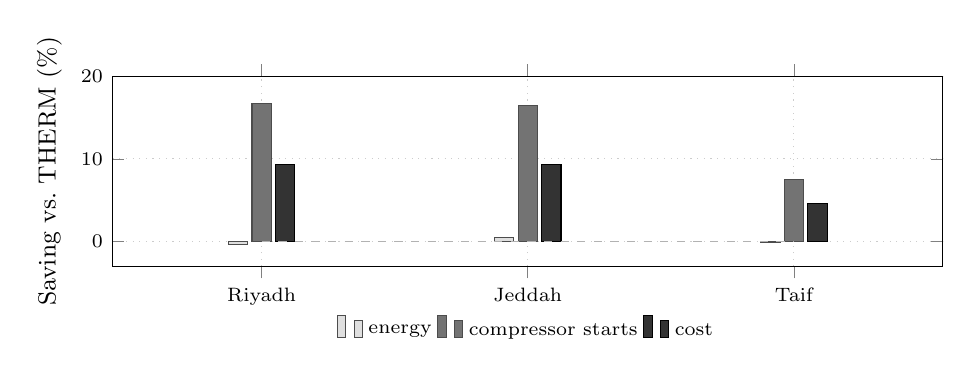
\begin{tikzpicture}
\begin{axis}[
  width=\columnwidth, height=4.0cm,
  ybar=1.5pt,
  bar width=7pt,
  grid=major, grid style={dotted,gray!40},
  tick label style={font=\scriptsize},
  label style={font=\small},
  ylabel={Saving vs.\ THERM (\%)},
  symbolic x coords={Riyadh,Jeddah,Taif},
  xtick=data,
  ymin=-3, ymax=20,
  enlarge x limits=0.28,
  legend style={at={(0.5,-0.22)},anchor=north,legend columns=3,
                font=\scriptsize,draw=none,fill=none},
]
\addplot+[draw=black!70,fill=gray!25]
  coordinates{(Riyadh,-0.3)(Jeddah,0.5)(Taif,-0.1)};
\addlegendentry{energy}
\addplot+[draw=black!70,fill=black!55]
  coordinates{(Riyadh,16.7)(Jeddah,16.4)(Taif,7.5)};
\addlegendentry{compressor starts}
\addplot+[draw=black,fill=black!80]
  coordinates{(Riyadh,9.3)(Jeddah,9.3)(Taif,4.6)};
\addlegendentry{cost}
\draw[gray!60,dashed] (axis cs:Riyadh,0) -- (axis cs:Taif,0);
\end{axis}
\end{tikzpicture}
\caption{The saving is a switching saving. For the tuned rule, the arm whose
energy and start columns Table~\ref{tab:main} reports in full, energy moves by
less than one point in either direction while compressor starts fall by $7.5$
to $16.7\%$ and cost by $4.6$ to $9.3\%$. Identity~\eqref{eq:duty_identity}
requires exactly this once mean occupied temperatures are matched: with the
mean fixed, the duty cycle and hence the energy are fixed too, and what is left
to recover is the per-start charge. Source:
Table~\ref{tab:main}.}
\label{fig:decomp}
\end{figure}


These figures replace the earlier version's headline, not refine it.

\emph{The saving is a switching saving.} Starts fall by $7.5$--$16.7\%$ under
TUNED while energy moves between $-0.3\%$ and
$+0.5\%$; in Riyadh and Taif the cost-optimal rule uses marginally \emph{more}
energy to buy fewer starts. Figure~\ref{fig:decomp} separates the three
quantities, and the contrast between its panels is the result: the energy panel
is flat and occasionally negative while the cost panel is not. This is what identity~\eqref{eq:duty_identity}
requires once mean temperatures are matched, and it is why starts and energy are
reported beside cost: neither depends on the tariff or on $\csw$, whereas cost
depends on both.

\emph{Commissioning the thermostat captures about half of what is available.}
TUNED needs no learning and no state beyond the zone temperature, yet reaches
$9.3\%$ in Riyadh and Jeddah against attainable clairvoyant schedules at
$18.1\%$ and $17.8\%$, and bounds of $19.8\%$ and $19.5\%$. Any
claim for a learned controller must be measured against TUNED, not THERM, and
the headroom it could occupy lies between $8.8$ and $9.7$ points in Riyadh and
between $8.5$ and $9.5$ in Jeddah, the interval set by them. That interval is
wide, and nothing in this paper's results closes it; what does close part of it
is a forecast, as Section~\ref{subsec:abl_component} shows.

\emph{Occupancy setback is the largest lever and it is climate-dependent},
raising the attainable figure by $7.7$ points in Riyadh, $8.0$ in Jeddah and
$6.5$ in Taif. The mechanism is not storage (the figure is unchanged when the
unoccupied limit is varied between $24$ and $32\,^\circ$C, because heat entering
during a setback must still be removed), but the reduced envelope gain while the
zone floats warm.

\emph{Taif behaves differently.} Its lower load leaves less for a pair of fixed
thresholds to exploit, so TUNED reaches only $4.6\%$ while a clairvoyant
schedule reaches $15.0\%$, the widest gap of the three cities, and the
standard deviation of that clairvoyant saving is $6.9$ points against $1.7$ in
Riyadh; Section~\ref{subsec:disc_precool} draws the mechanism. Three cities
are reported as three climates, not as evidence of generalisation across the
Kingdom.

Under the schedule announced for January 2027 ($0.21\,\SAR/\kWh$) every cost
figure falls---Riyadh TUNED $8.6\pm1.5\%$, Jeddah $8.6\pm1.3\%$, Taif
$4.3\pm3.5\%$, against a Lagrangian bound of $17.6\%$ in Riyadh---while the
energy and start savings are unchanged, because a
higher energy price dilutes a saving whose mechanism is a fixed charge per
start. Section~\ref{subsec:disc_tariff} develops this dependence, which is the
principal reason the figures here are lower than those reported in the earlier
version of this study.
 
\paragraph{Four withdrawals.}
\label{subsec:res_all}
The table of per-configuration costs under three cost models previously
reported here is withdrawn in full, with the GA and SA comparators evaluated
against it (the response letter sets out why); Tables~\ref{tab:main}
and~\ref{tab:sensitivity}(a) replace it, and the bound
of~\eqref{eq:dual_bound} replaces the metaheuristic comparators, applying to
any day-ahead solver as to any other mean-matched schedule. Second, the
attribution of the largest saving to tier-boundary pre-cooling is withdrawn:
the first block extends to $6{,}000\,\kWh$ per month against this account's
few hundred, so no boundary is approached, no cost-optimal schedule computed
here pre-cools, and a single weekly horizon is reported. Third, the claim that
per-zone cost rises with $N_z$ through coupling is withdrawn with the
conductance ratio quoted for it: a $4\times4$ grid's sixteen zones average
exactly one exposed face ($23.75\,$W/K, identical to the single zone), so
comparing per-zone cost across topologies measures face count, not coupling;
multi-zone results under this tariff, for a larger unit and a
$[23,25]\,^\circ$C band, are in~\cite{Faraj2026}, and none is reported here.
 
\section{State-of-the-Art Comparison and Ablation Study}
\label{sec:analysis}

Three questions remain after Section~\ref{sec:results}: how these figures
compare with published ones, which component of RBRL produces them, and what
can be said about computational cost.
Sections~\ref{subsec:sota}, \ref{subsec:abl_component}
and~\ref{subsec:abl_cost} take them in turn; the second answers with a negative
result and the third largely with a withdrawal.
 
\subsection{State-of-the-Art Comparison}
\label{subsec:sota}
 
Published RL-based HVAC studies differ in control type, building type, baseline, and climate.
Table~\ref{tab:sota} accounts for these with an explicit \emph{Basis} column.
 
\begin{table*}[t]
\centering
\caption{State-of-the-art comparison. The ``Basis'' column is essential
for interpreting saving figures.}
\label{tab:sota}
 
\setlength{\tabcolsep}{6pt} % uniform spacing
 
\begin{tabularx}{\textwidth}{
>{\raggedright\arraybackslash}X   % Reference
>{\centering\arraybackslash}X     % Year
>{\raggedright\arraybackslash}p{0.30\linewidth}  % Method
>{\centering\arraybackslash}X     % Saving
>{\raggedleft\arraybackslash}p{0.22\linewidth}  % Basis (right-aligned)
}
\toprule
Reference & Year & Method & Saving & Basis \\
\midrule
\cite{Azuatalam2020} & 2020 & Q-learning, whole-bldg & 22\% & vs.\ thermostat \\
\cite{Du2021b}        & 2021 & DDPG, multi-zone resid. & 15\% & vs.\ thermostat \\
\cite{Biemann2021}    & 2021 & SAC/TD3, continuous    & $>$10\% & vs.\ rule-based \\
\cite{Wang2024DRL}    & 2024 & DRL, continuous VAV    & 37\%$^{a}$ & vs.\ rule-based \\
\cite{Solinas2024}    & 2024 & Online RL, white-box   & 65\%$^{b}$ & vs.\ no control \\
\cite{Xue2025}        & 2025 & GA-MADDPG hybrid       & 6.7\%  & vs.\ rule-based \\
\midrule
\textbf{This work} & 2026 & Tuned rule, tariff in force, Riyadh & \textbf{9.3\%} & \textbf{vs.\ thermostat, iso-comfort, held out} \\
\textbf{This work} & 2026 & Clairvoyant schedule, same instance & \textbf{18.1\%} & \textbf{attainable; cooler than baseline in every window} \\
\textbf{This work} & 2026 & Lagrangian bound, same instance & $\mathbf{\le19.8\%}$ & \textbf{no mean-matched schedule beats it} \\
\textbf{This work} & 2026 & MPC, $24\,$h horizon, same instance & \textbf{8.4\%} & \textbf{causal; perfect forecast inside the horizon} \\
\textbf{This work} & 2026 & RBRL (PPO $+$ hard rules), Riyadh & \textbf{5.7\%}$^{c}$ & \textbf{vs.\ thermostat, iso-comfort, held out} \\
\bottomrule
\multicolumn{5}{l}{\footnotesize
$^{a}$Continuous VAV modulation in a simulated office: different hardware
and building type.}\\
\multicolumn{5}{l}{\footnotesize
$^{b}$Relative to a no-HVAC baseline; saving vs.\ thermostat is
substantially lower.}\\
\multicolumn{5}{l}{\footnotesize
$^{c}$Mean over five seeds; \emph{below} the tuned rule, and reported as a
negative result (Section~\ref{subsec:abl_component}).}
\end{tabularx}
\end{table*}
 
Comparison with published figures requires care, and the most informative comparison is not the most flattering one. Xue et al.~\cite{Xue2025}, whose protocol is closest to this one (a rule-based comparator, a cost objective, and no clairvoyant reference---report $6.7\%$, against the $9.3\%$ obtained here; the agreement to within three points is the meaningful result. The larger published figures differ in scope, not in degree, as the table's notes record. The figures reported here are additionally iso-comfort matched and held out, neither of which is standard in this literature, and both of which reduce the number; the clairvoyant bound is reported so that the remaining headroom is visible rather than implied. This is not a claim about the tariff now in force.
 
\subsection{Component and Cost Model Ablation}
\label{subsec:abl_component}
 
Table~\ref{tab:abl_component} ablates the rule layer and the learned component against each other, Riyadh, tariff in force.
 
\begin{table*}[t]
\centering
\caption{Component ablation, Riyadh, tariff in force, held-out windows, five
seeds. All rows except the first are comfort-matched to THERM's mean occupied
temperature; the no-rules row cannot be matched, since it leaves the band, and
is reported unmatched.
\textbf{The decisive row is the comparison between RBRL and a bare hysteresis
rule placed at the rule layer's own guard thresholds}
(Corollary~\ref{cor:rules_sufficient} in measured form;
Section~\ref{subsec:abl_component}). Degree-hours are counted while occupied.
$^{*}$MPC is causal, with a perfect forecast only inside its horizon and the
terminal thermal state priced as the dynamic programme prices it. Every MPC row
is matched window by window on the same criterion as the other arms (no warmer
than that window's own baseline), which is \emph{not} how an earlier version of
this table matched them; matching only the aggregate mean inflated the $24\,$h
figures by up to ten points and the $6\,$h figures by more. All rows are
solved on the dynamic programme's own $1601$-point grid with the ceiling
matched in $0.01\,^\circ$C steps; the $801$-point grid of the earlier version
returns costs $1.4$--$3.0\%$ lower under the identical protocol, so the
coarser grid flattered this arm. The match is one-sided (no warmer than the
baseline), so any residual mismatch over-cools and \emph{handicaps} this arm;
the largest residuals ($0.06$--$0.12$ K) occur in single shoulder-season
windows where the admissible ceilings step coarsely.
$^{\ddagger}$In Taif the $24$ and $48\,$h arms match in only six of the seven
windows: in the seventh no ceiling brings the mean occupied temperature down
to the baseline's, so the arm cannot be matched there at all and that window
is excluded. The Taif figures are correspondingly less comparable than the others.
Bold marks the rows and quantities the argument turns on, not the best
value in a column: the cheapest arm here is the clairvoyant schedule, which is
a reference, not a controller. The RBRL row is a five-seed mean, and its
agreement with the hysteresis row is a trajectory identity, not a statistical
resemblance: in nine of the ten Riyadh and Jeddah runs the learned policy's
cost equals the hysteresis's in every individual window (maximum per-window
difference $0.000\,\SAR$), and in the tenth it is dearer by at most
$0.024\,\SAR$/day in one window; a significance test on identical numbers
would be vacuous, which is why none is quoted for this pair.}
\label{tab:abl_component}
\setlength{\tabcolsep}{3.5pt}
\resizebox{\textwidth}{!}{%
\begin{tabular}{@{}lrrrr@{}}
\toprule
Variant & $\Jbar/N_z$ & $f_s$ & deg-h & Saving \\
\midrule
PPO alone, \emph{no rule layer} & $1.1201$ & $4.13$ & $\mathbf{0.085}$ & $+0.1\%$ \\
THERM, guards at band edges & $1.1183$ & $4.10$ & $0.000$ & --- \\
RBRL (PPO $+$ hard rules R1--R2) & $1.0583$ & $3.70$ & $0.000$ & $5.7\%$ \\
Hysteresis at the guard thresholds,\\
\quad \emph{no learned policy at all} & $\mathbf{1.0576}$ & $\mathbf{3.69}$ & $\mathbf{0.000}$ & $\mathbf{5.8\%}$ \\
TUNED, switch points free of guards & $1.0170$ & $3.43$ & $0.000$ & $9.3\%$ \\
\midrule
CLV, best schedule found & $0.9174$ & $2.76$ & $0.001$ & $18.1\%$ \\
\quad\emph{bound} (\ref{eq:dual_bound}) & $\ge0.8969$ & --- & --- & $\le19.8\%$ \\
\midrule
\multicolumn{5}{@{}l}{\emph{Across cities, comfort-matched saving vs.\ THERM:}} \\
\quad RBRL (five-seed mean) & \multicolumn{4}{r}{Riy $5.7\%$\,/\,Jed $5.8\%$\,/\,Tai $7.6\%$} \\
\quad guard hysteresis, no learning & \multicolumn{4}{r}{Riy $5.8\%$\,/\,Jed $5.8\%$\,/\,Tai $7.6\%$} \\
\quad TUNED & \multicolumn{4}{r}{Riy $9.3\%$\,/\,Jed $9.3\%$\,/\,Tai $4.6\%$} \\
\quad MPC, $6\,$h horizon\rlap{$^{*}$} & \multicolumn{4}{r}{Riy $-4.0\%$\,/\,Jed $-4.7\%$\,/\,Tai $-18.2\%$} \\
\quad MPC, $24\,$h horizon\rlap{$^{*}$} & \multicolumn{4}{r}{Riy $8.4\%$\,/\,Jed $5.9\%$\,/\,Tai $2.9\%$\rlap{$^{\ddagger}$}} \\
\quad MPC, $48\,$h horizon\rlap{$^{*}$} & \multicolumn{4}{r}{Riy $10.8\%$\,/\,Jed $9.5\%$\,/\,Tai $4.3\%$\rlap{$^{\ddagger}$}} \\
\quad MPC, $24\,$h, \emph{inside} R1--R2 & \multicolumn{4}{r}{Riy $3.1\%$} \\
\quad CLV, best schedule found & \multicolumn{4}{r}{Riy $18.1\%$\,/\,Jed $17.8\%$\,/\,Tai $15.0\%$} \\
\quad \emph{bound} (\ref{eq:dual_bound}) & \multicolumn{4}{r}{Riy $\le19.8\%$\,/\,Jed $\le19.5\%$\,/\,Tai $\le20.2\%$} \\
\quad \textbf{price of the guarantee} & \multicolumn{4}{r}{$\mathbf{3.6}$\,/\,$\mathbf{3.5}$\,/\,$\mathbf{-3.1}$ \textbf{points}} \\
\bottomrule
\end{tabular}}
\end{table*}
 
Four things follow, and the second is the central empirical result of this
revision.

\emph{The rule layer is necessary, and it is what makes the result
reproducible.} Without R1 and R2 the agent violates the band in \emph{every}
seed ($0.021$, $0.116$, $0.273$ occupied degree-hours) despite the quadratic
comfort penalty in its reward, and buys nothing for it: the saving is
$+0.1\pm5.3\%$, indistinguishable from the thermostat and negative in three of
five seeds. The dispersion is the second half of the point: with the rule
layer the seed standard deviation of the saving is $0.00$ points in Jeddah,
where all five seeds give identical trajectories, and $0.21$ in Riyadh, where
four of five do; without it, $5.3$ percentage points: an order of magnitude larger, and
larger than any margin achieved here over the tuned rule. Comfort matching is undefined for this ablation, since
the policy leaves the band and its mean occupied temperature differs by seed
($22.90$--$23.11\,^\circ$C across the five); the row is reported unmatched.

\emph{The learned component is inconsequential, as
Corollary~\ref{cor:rules_sufficient} predicts.} A PPO agent trained for
$2\times10^{5}$ steps under the rule layer never costs less than a bare
hysteresis rule placed at the rule layer's own guard thresholds, and usually
costs exactly the same. Against the rule's $1.0576$ and $0.9354\,\SAR$/zone/day
in Riyadh and Jeddah, the five seeds give $1.0610$ once and $1.0576$ four
times over in Riyadh, and $0.9354$ five times over in Jeddah: nine of the ten
runs reproduce the rule's cost \emph{in every individual window}, and the
tenth is $0.0034$ above it. What remains for a learned policy to find is bounded and small: the residual
is $0.59\%$ in Riyadh and $0.02\%$ in Jeddah (Remark~\ref{rem:cor_scope}),
smaller than one seed's dispersion, and PPO recovers none of it.

\emph{A day of lookahead is not what is missing; the rule layer is.} An earlier
version of this analysis read the headroom off a diagonal (bare hysteresis at
one corner, a $24\,$h receding-horizon controller at the other) and blamed
the agent's one-hour observation window; a diagonal cannot separate two
factors. The completed $2\times2$, every cell matched window by window to its
own baseline mean, gives the opposite reading in Riyadh:

\begin{center}\small
\begin{tabular}{@{}lrr@{}}
\toprule
 & no rules & rules R1--R2 \\
\midrule
no lookahead & $9.3\%$ (TUNED) & $5.8\%$ (hysteresis) \\
$24\,$h lookahead & $8.4\%$ (MPC) & $3.1\%$ \\
clairvoyant & $18.1\%$ & $6.3\%$ \\
\bottomrule
\end{tabular}
\end{center}

Reading down the columns, a day of lookahead is worth nothing in either: $9.3$
to $8.4$ without the rules, and $5.8$ to $3.1$ with them. Reading across the
rows, removing the rule layer is worth $3.5$ points with no lookahead and $5.3$
with a day of it. What does pay is foresight at the scale of the plant's time
constant and beyond, but only
outside the rules: the clairvoyant row stands $9.7$ points above the $24\,$h
row without them and $3.2$ points above it with them, and inside the rules even
unlimited foresight reaches just $6.3\%$---half a point above a bare hysteresis.
That half-point is the whole of what any policy, learned or otherwise, could
recover within the rule-admissible class. At a $6\,$h horizon the receding-horizon controller is worse than the
baseline outright, at $-4.0\%$ in Riyadh, $-4.7\%$ in Jeddah and $-18.2\%$ in
Taif: a horizon far shorter than the plant's $56\,$h time constant commits the
compressor on evidence that has not yet arrived, and pays the switching charge
for it.

The $24\,$h parity is tested, not asserted. On the seven paired windows the
exact Wilcoxon gives $p=0.94$ in Riyadh: the tuned rule's mean edge
($+0.9$ points) comes entirely from the one shoulder-season window in which
the matched arm is also over-cooled by $0.09\,^\circ$C, the median difference
runs the other way ($-1.6$ points, four of seven windows favouring the
receding-horizon arm), and the BCa interval on the difference,
$[-1.6,+5.3]$ points, excludes only differences beyond about five points. In
Jeddah the rule is significantly \emph{better} than a day of lookahead:
$+3.4$ points, $p=0.047$, interval $[+0.7,+5.6]$. At $48\,$h the
receding-horizon arm draws level or slightly ahead ($-1.6$ points in Riyadh,
$p=0.22$; $-0.2$ points, $p=1.0$ in Jeddah), which places the horizon at
which lookahead starts to pay near the plant's $56\,$h time constant,
consistent with the clairvoyant bracket.

Two qualifications are owed. The $24\,$h rows use a perfect forecast inside the
horizon, so they are information-idealised \emph{upper} estimates, and the
direction matters: forecast error would lower the $24\,$h rows, and the
conclusion those rows support is that a day of lookahead buys nothing over the
tuned rule---an idealisation that favours the arm being dismissed
\emph{strengthens} the dismissal, which is why no forecast-error study is
needed to sustain it and none is reported. And the rule-constrained cells are confounded, because
the occupied cap that matches comfort also sets the guard threshold at
$\mathrm{cap}-\epsilon_{\mathrm{hot}}$, so tightening the match tightens the
rules. The $3.1\%$ cell should therefore be read as an upper estimate of the
cost of the rule layer at matched comfort, not as a clean measurement of it.
Separating the two would require a comfort-matching device independent of the
guard thresholds, which is required work.

\emph{The comfort guarantee has a price, but not everywhere.} In Riyadh and
Jeddah TUNED, free of the guards, is cheaper---$9.3\%$ against $5.7\%$ and
$5.8\%$---so the hard rules cost $3.5$ to $3.6$ percentage points. In Taif the
ordering reverses: the guard-constrained policy saves $7.6\%$ against TUNED's
$4.6\%$, at a closer comfort match. The reason is protocol, not physics, and
not to the architecture's credit: TUNED's switch points are admitted against
the \emph{tuning} windows, which in Taif excludes the lower switch-off point
the guards impose, while the ceiling that places the guards was searched on
the \emph{held-out} windows. The two arms are fitted under different
protocols, and the reversal measures that difference at least as much as
anything about guards; it is reported as an artefact that matching every
arm's ceiling on the tuning windows alone would remove, not as evidence that
a rule layer is free. The defensible reading is narrower---the guards are not
\emph{reliably} costly across climates---and what they buy everywhere is a
guarantee: nothing in TUNED's construction prevents an over-temperature
violation on unseen weather, whereas R1 and R2 exclude one by construction.

Taif requires care, and the care is instructive. At a ceiling of
$23.79\,^\circ$C the saving is $7.6\pm3.8\%$ at a mean occupied temperature
$0.004\,^\circ$C \emph{below} the baseline's, with zero over-temperature
degree-hours; that is the figure tabulated. It is not a unique point but the
closest-matched member of a family: seven ceilings on the $0.01\,^\circ$C scan
grid satisfy the admission rule ($|\Delta T|\le0.03\,^\circ$C, zero
over-temperature degree-hours), and their savings span $6.2$--$8.6\%$. The
spread is not estimation noise. The saving moves in near-steps with the daily
start count ($6.2\%$ at $2.08$ starts/day, $7.6\%$ at $2.02$, $8.6\%$ at
$1.98$): a $0.01\,^\circ$C ceiling change either does or does not remove one
start from some window, so the admissible family samples a staircase, and any
single Taif figure carries an implicit $\pm1.2$-point grid quantisation that
the Riyadh and Jeddah figures, with their denser cycling, do not. Conclusions
drawn from Taif in this paper are therefore stated only at the family level. It carries $0.350$ degree-hours of
under-temperature in the $16$~October window, where the outdoor minimum reaches
$16\,^\circ$C, against the baseline's $0.156$ there for the same reason, so the
comparison is like-for-like in kind. An earlier ceiling of $23.93\,^\circ$C,
reached by a bisection that is not monotone once an excursion is one the plant
cannot correct, left the policy $0.075\,^\circ$C warm and its apparent saving
at $12.4\%$. That a $0.079\,^\circ$C difference in setpoint is worth nearly
five percentage points is itself the argument for matching.

Table~\ref{tab:sensitivity} isolates the two economic parameters. Panel~(a)
gives the tariff dependence; the $13.1\%$ figure previously reported for
training under an inaccurate tariff model is withdrawn, having been obtained
from irreproducible runs under a superseded schedule, and what survives is the
qualitative point that a smooth approximation of a tariff containing a boundary
misprices every schedule crossing it: a smooth model (Model~E) never represents
the discrete tier boundary, so the substitution changes the incentive structure
qualitatively, though under a constant marginal price all three cost models
reduce to the same objective up to scale and cannot be distinguished at all
(Proposition~\ref{prop:path}). For this dwelling that case does not
arise, the marginal price being constant under both present schedules. Panel~(b)
is consistent with Remark~\ref{rem:csw}: higher $\csw$ produces fewer, longer
on-phases, as Proposition~\ref{prop:structure} requires.

Panel~(c) is the sensitivity that matters most, and it was missing from the
earlier version of this study. The saving depends more strongly on the
\emph{baseline's} deadband than on any parameter of the controller: holding the
comfort band fixed, the fixed guard hysteresis saves $34.3\%$ against a
$0.50\,^\circ$C baseline and $-3.4\%$ against a $1.25\,^\circ$C one, a swing of
$38$ points across the admissible interval. Three things follow. The reported
figure is a statement about a \emph{pair}, controller and comparator, and not
about the controller alone. The adopted $\deadband=1\,^\circ$C sits near the
upper end of the admissible interval $[0.375,1.25]\,^\circ$C, so the baseline is
specified close to the most favourable setting available to it, which is the
right direction for a comparator and a stronger defence than calling it
representative. And the deadband of the installed stock is not measured here:
it is the single most valuable field measurement anyone could make against this
study, because at $1.25\,^\circ$C the saving reverses sign.
 
\begin{table*}[t]
\centering
\caption{Sensitivity of the reported saving, on the held-out protocol (Riyadh,
seven windows, mean $\pm$ sd of the paired saving). (a)~Tariff schedule, at
$\csw=0.15\,\SAR$. (b)~Switching cost, at the tariff in force. ``Switching
share'' is $\csw f_s/J$ for THERM, the fraction of the baseline's cost
attributable to compressor starts. (c)~The \emph{comparator's} deadband at a
fixed $[22,24]\,^\circ$C band, which is the parameter the reported saving
depends on most strongly and the one the earlier version of this study did not
examine.}
\label{tab:sensitivity}

\setlength{\tabcolsep}{4pt}

\begin{subtable}{\textwidth}
\caption*{\textbf{(a) Tariff schedule}}
\begin{tabularx}{\textwidth}{@{}Xcccc@{}}
\toprule
Schedule & $\SAR/\kWh$ & Sw.\ share & TUNED & bound \\
\midrule
Pre-2018 Tier~1 & $0.05$ & $81.5\%$ & $13.6{\pm}2.1\%$ & $\le29.2\%$ \\
\textbf{In force} & $\mathbf{0.18}$ & $\mathbf{55.0\%}$ & $\mathbf{9.3{\pm}1.6\%}$ & $\mathbf{\le19.8\%}$ \\
From Jan 2027 & $0.21$ & $51.2\%$ & $8.6{\pm}1.5\%$ & $\le18.5\%$ \\
\bottomrule
\end{tabularx}
\end{subtable}

\vspace{6pt}

\begin{subtable}{\textwidth}
\caption*{\textbf{(b) Switching cost}}
\begin{tabularx}{\textwidth}{@{}Xccc@{}}
\toprule
$\csw$ (SAR) & Sw.\ share & THERM $J$ & TUNED \\
\midrule
$0.00$ & $0.0\%$ & $0.5030$ & $0.1{\pm}0.1\%$ \\
$0.05$ & $29.0\%$ & $0.7081$ & $4.9{\pm}1.0\%$ \\
$\mathbf{0.15}$ & $\mathbf{55.0\%}$ & $\mathbf{1.1183}$ & $\mathbf{9.3{\pm}1.6\%}$ \\
$0.30$ & $71.0\%$ & $1.7336$ & $11.9{\pm}1.9\%$ \\
$0.60$ & $83.0\%$ & $2.9642$ & $13.9{\pm}2.2\%$ \\
\bottomrule
\end{tabularx}
\vspace{1pt}
{\footnotesize\raggedright The clairvoyant column previously reported in this
panel is withdrawn: it came from the superseded pointwise-capped device, and
its comfort match converged on only $2$ of the $7$ windows at $\csw=0$ and $6$
of $7$ at $0.05$, so the column was not comparable row to row. The dependence
the panel exists to show is carried by the tuned rule, whose saving falls to
$0.1\%$ when the switching charge is removed.\par}
\end{subtable}

\vspace{6pt}

\begin{subtable}{\textwidth}
\caption*{\textbf{(c) The baseline's deadband, at fixed comfort band}}
\begin{tabularx}{\textwidth}{@{}Xccccc@{}}
\toprule
$\deadband$ ($^\circ$C) & adm. & THERM $f_s$ & THERM deg-h & Guard hyst. & TUNED \\
\midrule
$0.50$ & yes & $7.37$ & $0.000$ & $34.3\%$ & $32.1{\pm}0.6\%$ \\
$0.75$ & yes & $5.22$ & $0.000$ & $18.1\%$ & $3.4{\pm}2.3\%$\rlap{$^\ddagger$} \\
$\mathbf{1.00}$ & \textbf{yes} & $\mathbf{4.10}$ & $\mathbf{0.000}$ & $\mathbf{5.8\%}$ & $\mathbf{9.3{\pm}1.6\%}$ \\
$1.25$ & yes & $3.45$ & $0.000$ & $-3.4\%$ & $-2.2{\pm}1.6\%$ \\
$1.50$ & \textbf{no} & $2.96$ & $0.132$ & $-11.5\%$ & --- \\
\bottomrule
\end{tabularx}
\vspace{1pt}
{\footnotesize\raggedright Admissibility is by the corrected
bound~\eqref{eq:deadband_condition}, $0.375\le\deadband\le1.25\,^\circ$C; the
band-width bound alone would admit $1.50\,^\circ$C, at which the baseline leaks.
``Guard hyst.'' is the \emph{fixed} controller of
Section~\ref{subsec:abl_component} evaluated against each baseline, and is
monotone in $\deadband$. $^\ddagger$TUNED is re-tuned at each $\deadband$ and is
\emph{not} monotone, for the same reason as the capacity sweep: the iso-comfort
constraint collapses the admissible set of switch points at some deadbands, so
the tuner is forced onto a narrow pair. The monotone column is the one to read
for the mechanism.\par}
\end{subtable}

\end{table*}
 
\subsection{Scalability}
\label{subsec:abl_cost}
 
\textbf{The zone-count and computational-scalability table previously reported
here is withdrawn in full}, for the reasons the response letter sets out, and
with it any claim about training cost or embedded deployability.

What \emph{can} be reported is inference cost, measured for this revision on
disclosed hardware. All timings below are medians with inter-quartile ranges,
taken with \texttt{time.perf\_counter} on an Intel Xeon at $2.10\,$GHz
($2$ logical cores, no thread pinning, $7.8\,$GiB), Linux kernel
$6.18.44$, Python $3.13.18$, NumPy $2.5.3$ on scipy-openblas, SciPy $1.18.1$,
PyTorch $2.15.0{+}$cpu and Stable-Baselines3 $2.9.2$. \textbf{No GPU was
used.} Peak resident memory of the measuring process was $282\,$MiB by
\texttt{getrusage}; this is a memory measurement and is not to be confused
with a parameter count, a conflation that is what forced the withdrawal of the
earlier table.

The rule layer, the arithmetic a deployed RBRL controller performs at each
interval, decides in $1.07\,\mu$s at one zone and $1.06\,\mu$s at sixteen
(IQR $\le0.04\,\mu$s), the flatness reflecting that at these sizes the cost is
interpreter overhead, not the $O(N_z)$ comparison the rule implies. The
receding-horizon controller, which re-solves the full Bellman recursion over
its horizon at every interval on an $801$-point grid, takes $8.6\,$ms per
decision at a $24\,$h horizon and $2.1\,$ms at $6\,$h. Against a control step
of $900\,$s that is a margin of five orders of magnitude, so the standing
objection that such a controller ``requires an on-line solver at each step,
which limits embedded deployment'' does not bite on the single-zone instance
evaluated here and should not be offered as a reason to prefer a learned policy
at this scale. The claim is deliberately narrow: $8.6\,$ms on a server-class
core is not $8.6\,$ms on a microcontroller, and no embedded-deployment claim is
made.

The scalability question that \emph{is} settled here is structural, not
empirical. A clairvoyant dynamic programme over $N_z$ coupled zones carries a
temperature grid of $G=1{,}601$ points per zone, so $G^{N_z}$ thermal states;
each is held for every configuration of the previous action vector, since the
switching charge makes each zone's cost depend on its own previous state,
giving $G^{N_z}2^{N_z}$ states; and each is evaluated against $2^{N_z}$ joint
actions. The backward pass therefore touches $G^{N_z}4^{N_z}$ transitions
per interval: $4.1\times10^{7}$ at two zones, $2.6\times10^{11}$ at three and
$8.0\times10^{60}$ at sixteen. These are
arithmetic, not timings, and they are the reason no multi-zone optimality
reference appears in this paper: the obstruction is the formulation, not the
machine. It is also why the bracket of Section~\ref{subsec:bound}, which
carries this paper's entire epistemic frame, is a single-zone result and is not
extrapolated. Multi-zone results under the same tariff, obtained with a
learned policy rather than a dynamic programme, are reported
in~\cite{Faraj2026}; that study uses a larger split unit ($1.8\,$kW input
against $0.670\,$kW here), a $[23,25]\,^\circ$C band and Jeddah profiles only,
and Section~\ref{subsec:disc_band} shows the band alone moves the reported
saving by ten points, so its figures are not directly comparable with these.
 
\section{Discussion}
\label{sec:discussion}

The results invite three questions: why the cities differ, why the cost models do
not, and what the reported saving actually depends on. The last is the most
consequential and is taken last.
 
\subsection{Pre-Cooling Headroom, Inter-Zone Coordination, and Climate}
\label{subsec:disc_precool}
 
The difference between the cities is not primarily an algorithmic one; it
reflects available thermal headroom and the baseline's cycling rate. Riyadh and
Jeddah behave alike at both ends of the range ($9.3\%$ with the tuned rule,
$18.1\%$ and $17.8\%$ with clairvoyance), so what separates them is not how much
is available but nothing at all. Taif is the informative case: the tuned rule
recovers $4.6\%$ there while a clairvoyant schedule recovers $15.0\%$, the
widest gap of the three. A low and variable load does not mean little to win; it
means the switch points that win it move from week to week, which a pair of
fixed thresholds cannot follow.
Riyadh's $12.7\,$K cooling-season diurnal swing buys a longer off-leap: the zone
free-floats further before the band forces the compressor on, so fewer starts
are needed over a day. What it does \emph{not} buy, in this model, is
pre-cooling. Remark~\ref{rem:energy_identity} shows that under a constant
marginal price running colder than necessary raises consumption, and no
pre-cooling appears in any cost-optimal schedule computed here. Nor does the
model represent a temperature-dependent coefficient of performance, which is
constant at $2.985$ throughout (Table~\ref{tab:params}) and is listed among the
omissions in Section~\ref{subsec:limits}; in a plant whose efficiency fell with
outdoor temperature, deferring runtime out of the afternoon would carry a
further benefit this study cannot quantify.
Jeddah's overnight outdoor temperature falls little, averaging $27.1\,^\circ$C over the year and $29$--$32\,^\circ$C through the cooling season, which gives a swing of only $8.4\,$K; there is correspondingly less surplus for pre-loading.
 
For hot-humid coastal cities the implication is that passive envelope improvements (thicker walls, lower SHGC glazing, external shading) that increase $\Cth$ or reduce $\Lambda_i$ enlarge the off-leap duration $\taum$ (equation~\eqref{eq:cycle_cost}), creating the buffer that pre-cooling requires~\cite{AlReshidi2024}.
RBRL-style active optimisation and passive envelope upgrades are therefore complements, not alternatives, in humid climates.
 
Inter-zone coordination is retained in the formulation but not measured here.
The effective inter-zone temperature $\Tiz{i}^{(t)}$ of~\eqref{eq:tiz} is retained in the state as the anticipatory signal for multi-zone staggering, but no multi-zone numerical result is reported in this version, so no claim is made for its measured effect.
Without $\Tiz{i}^{(t)}$ in the state the agent cannot anticipate a neighbour's heat cascade, so more R1 overrides are triggered, each incurring $\csw=0.15\,\SAR$ and breaking the complete-cycle structure of Proposition~\ref{prop:structure}. An ablation isolating this term is identified as required work in Section~\ref{subsec:disc_limits}; the present tables do not separate it.
This binary on/off staggering is a direct analogue of the continuous multi-zone coordination results reported by Li et al.~\cite{Li2024MZ}.
 
\subsection{Robustness of the Reported Results}
\label{subsec:robustness}

%% GENERATED by rbrl/gen_figs.py from results/T6_per_window.csv.
%% Do not edit by hand; regenerate.
\begin{figure}[t]
\centering
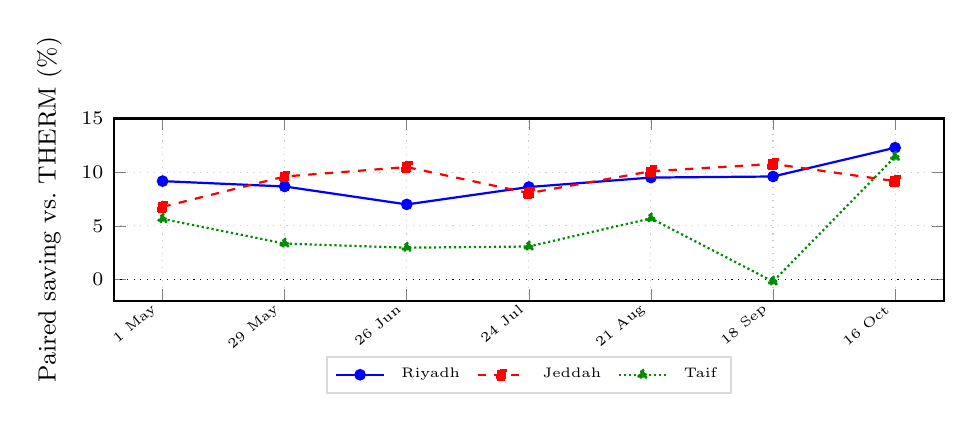
\begin{tikzpicture}
\begin{axis}[
  width=\linewidth, height=3.9cm,
  grid=major, grid style={dotted,gray!40},
  tick label style={font=\scriptsize},
  label style={font=\small},
  legend style={at={(0.5,-0.30)},anchor=north,legend columns=3,
                font=\tiny,draw=gray!30,column sep=4pt},
  thick,
  xmin=0.6, xmax=7.4, xtick={1,...,7},
  xticklabels={1 May,29 May,26 Jun,24 Jul,21 Aug,18 Sep,16 Oct},
  xticklabel style={font=\tiny,rotate=40,anchor=east},
  ylabel={Paired saving vs.\ THERM (\%)},
  ymin=-2, ymax=15,
]
\addplot[black,dotted,thin,forget plot] coordinates{(0.6,0)(7.4,0)};
\addplot[blue,thick,mark=*,mark size=1.7pt]
  coordinates{(1,9.16)(2,8.66)(3,6.99)(4,8.61)(5,9.49)(6,9.59)(7,12.27)};
\addlegendentry{Riyadh}
\addplot[red,thick,dashed,mark=square*,mark size=1.7pt]
  coordinates{(1,6.76)(2,9.59)(3,10.47)(4,8.04)(5,10.08)(6,10.76)(7,9.16)};
\addlegendentry{Jeddah}
\addplot[green!55!black,thick,densely dotted,mark=triangle*,mark size=2pt]
  coordinates{(1,5.64)(2,3.34)(3,2.96)(4,3.07)(5,5.69)(6,-0.19)(7,11.43)};
\addlegendentry{Taif}
\end{axis}
\end{tikzpicture}
\caption{Paired saving on each held-out window, tariff in force. Each window is
differenced against its \emph{own} baseline run, because the baseline's cost
varies by a factor of $1.9$ across the season; a saving quoted against the
seasonal mean would carry a spurious dispersion. Riyadh and Jeddah are stable
across the season ($\pm1.6$ and $\pm1.4$ points); Taif, the mild-climate site,
is not, and includes one window at $-0.2\%$ where the tuned rule is no better
than the baseline. Source: the project repository
(Section~\ref{sec:data}).}
\label{fig:season}
\end{figure}


A single headline figure can be an artefact of one favourable setting, so the
saving is probed along every axis the model exposes, and each is reported as a
table, not asserted. Training stochasticity: five seeds per city, no seed
discarded and no best-of-$n$ selection; with the rule layer the seed standard
deviation of the saving is $0.00$ (Jeddah, all five seeds identical) to $0.21$
percentage points (Riyadh), and without it $5.3$
(Table~\ref{tab:abl_component}). Taif's seeds are excluded from this statement
because its matching bisection does not converge
(Section~\ref{subsec:abl_component}), so its across-seed spread measures the
cap staircase, not training stochasticity. Weather: seven held-out windows spanning
1~May--23~October, with the paired dispersion reported in
Table~\ref{tab:main} and window by window in Figure~\ref{fig:season}, which also
shows the one Taif window where the tuned rule is no better than the baseline.

\paragraph{Statistical treatment of the paired comparisons.}
The seven held-out windows are \emph{paired}, every arm running on the same
weeks, so comparisons are made on within-window differences, each carrying an
exact two-sided Wilcoxon signed-rank test on the paired costs, an exact sign
test as a distribution-free cross-check, and a $95\%$ BCa bootstrap interval
($2\times10^{4}$ resamples). At $n=7$ the smallest attainable Wilcoxon $p$ is
$2/2^{7}=0.016$, reached only when all seven differences share a sign: the
tests certify a sign but cannot resolve a small difference, a non-significant
result is an absence of evidence at this sample size, never evidence of
equivalence, and the interval is the operative statement. On this treatment the positive claim holds in every city:
TUNED beats THERM in all seven windows in Riyadh ($9.3\%$, BCa
$[8.4,10.6]$, $p=0.016$) and Jeddah ($9.3\%$, $[8.1,10.1]$, $p=0.016$), and in
six of seven in Taif ($4.6\%$, $[2.5,7.8]$, $p=0.031$). The comparisons
\emph{between} optimising arms (TUNED against the receding-horizon controller,
RBRL against the guard hysteresis) are stated with their intervals in
Section~\ref{subsec:abl_component}, where the equivalence they suggest is
bounded, not asserted.
Climate: three sites, the tuned rule spanning
$4.6$--$9.3\%$ against attainable clairvoyant schedules of $15.0$--$18.1\%$.
Orientation: the headline zone faces south, and re-running the full protocol
in Riyadh with the glazed face turned to each cardinal direction (identical
envelope, plant and windows; tune grid $0.02\,^\circ$C) gives $7.2\%$ north,
$5.7\%$ east, $9.5\%$ south and $11.3\%$ west, comfort-matched to within
$0.051\,^\circ$C in the worst arm. The south face is mid-family, not a best case: the harsher west face yields
the \emph{largest} saving, its tuned rule removing the most starts
($0.87$/day against $0.69$ south, $0.46$ east). The south row's $9.5\%$
differs from the headline $9.3\%$ only through the finer tune grid---the Taif
quantisation again---so orientation conclusions are stated at family level,
$5.7$--$11.3\%$.
Thermal capacity:
Table~\ref{tab:timestep}(b), over admissible capacities only. Actuation interval:
Table~\ref{tab:timestep}. Tariff and switching cost:
Table~\ref{tab:sensitivity}, and the comparator's own deadband,
Table~\ref{tab:sensitivity}(c), which moves the saving more than any axis
above. Comfort: zero over-temperature degree-hours in every reported row. No claim is made about dependence on zone count or adjacency: the
study that previously supported one is withdrawn and no multi-zone result is
regenerated here.

\paragraph{Weather year.}
Every table above runs on one TMYx record per city, and a typical year is by
construction not any year that occurred, so the inter-annual spread of the
saving is measured rather than assumed: fifteen actual years per city
(2009--2023, ERA5 reanalysis, the same plane-of-array transposition), from
which the hottest, median and mildest by cooling degree-days are run two ways.
\emph{Transfer} applies the TMYx-tuned thresholds unchanged, which is what a
rule commissioned once experiences; \emph{re-tuned} re-runs the full protocol
inside the year. The transferred rule is strikingly stable where cooling
dominates: across the extremes of fifteen real years it returns
$9.4$--$10.5\%$ in Riyadh and $9.1$--$9.4\%$ in Jeddah against each year's own
baseline, a spread smaller than a single year's across-window dispersion (the
mild Riyadh year carries $1.0\,^\circ$C$\cdot$h of excursion, so its
$10.5\%$ takes a small comfort credit). In Taif it spans $1.5$--$4.3\%$, the
mild year collapsing for the documented reason: a mild year in a mild climate
free-floats \emph{below} the band ($64\,^\circ$C$\cdot$h that no cooling-only
plant can correct), leaving little to save. The re-tuned arm is erratic in an
instructive way: in several years the per-window $\pm0.03\,^\circ$C admission
rule rejects every candidate (in the mildest Riyadh year, all of them, even on
a $0.02\,^\circ$C grid) while the transferred thresholds it would have
rejected perform at the TMYx level---what fails to transfer across years is
the \emph{admission protocol}, not the rule family. ERA5 is a reanalysis on a
$0.25^\circ$ cell, so these runs measure spread at fixed method and plant; the
TMYx figures remain the reported ones.

\paragraph{Calibration status.}
No measured consumption or indoor-temperature record was available for a
dwelling of this description, so the thermal model is \emph{uncalibrated}: it is
a reference model in the sense of ASHRAE Guideline 14, parameterised from the
Saudi Building Code envelope requirements and from manufacturer rated capacity
and efficiency, and not fitted to or validated against measurements from any
particular building. The hourly goodness-of-fit indices that Guideline 14 would
require of a calibrated model, $\mathrm{CV(RMSE)}$ and $\mathrm{NMBE}$ against
metered data, are therefore not reported, because there is no measured series
against which to compute them, and a calibration claim is not made anywhere in
this paper. Two consequences follow and are observed throughout: no absolute
figure here (a consumption, a cost, a trajectory) should be read as a
prediction for a real dwelling; and every quantitative claim is a
\emph{relative} comparison on one common model at a matched mean, a form in
which a shared bias in envelope, capacity or weather affects both arms alike
and largely cancels. What a shared bias does not cancel is the
\emph{sensitivity} of the saving to its governing parameters, which is why the
tariff, the switching cost, the capacity and above all the comparator's
deadband are swept, not assumed, and why Section~\ref{subsec:disc_limits}
names field measurement of the installed stock's deadband as the single
measurement that would most change these results.

\subsection{What Governs the Saving: the Band and the Tariff}
\label{subsec:disc_band}
\label{subsec:disc_tariff}
\label{subsec:disc_modele}

%% GENERATED by rbrl/gen_figs.py from results/T4_tariff.csv.
%% Do not edit by hand; regenerate.
\begin{figure}[t]
\centering
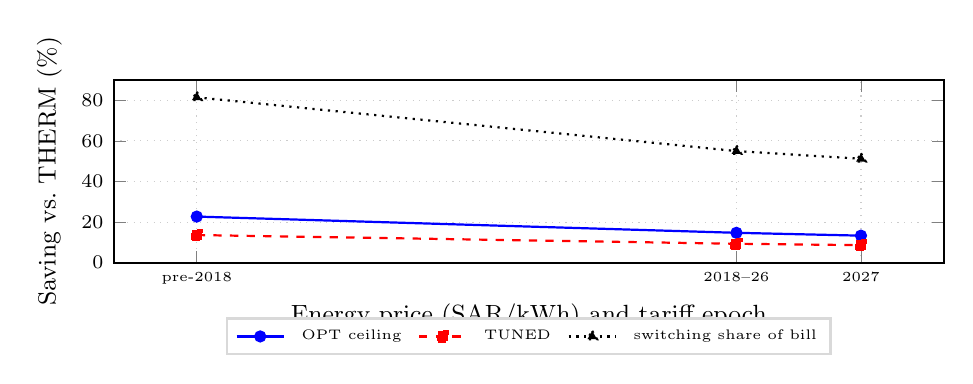
\begin{tikzpicture}
\begin{axis}[
  width=\linewidth, height=3.9cm,
  grid=major, grid style={dotted,gray!40},
  tick label style={font=\scriptsize},
  label style={font=\small},
  legend style={at={(0.5,-0.30)},anchor=north,legend columns=3,
                font=\tiny,draw=gray!30,column sep=4pt},
  thick,
  xtick={0.05,0.18,0.21}, xticklabels={pre-2018,2018--26,2027},
  xticklabel style={font=\tiny},
  xmin=0.03, xmax=0.23,
  xlabel={Energy price (\SAR/\kWh) and tariff epoch},
  ylabel={Saving vs.\ THERM (\%)},
  ymin=0, ymax=90,
]
\addplot[blue,thick,mark=*,mark size=1.8pt]
  coordinates{(0.05,22.7)(0.18,14.7)(0.21,13.3)};
\addlegendentry{OPT ceiling}
\addplot[red,thick,dashed,mark=square*,mark size=1.8pt]
  coordinates{(0.05,13.6)(0.18,9.3)(0.21,8.6)};
\addlegendentry{TUNED}
\addplot[black,dotted,thick,mark=triangle*,mark size=2pt]
  coordinates{(0.05,81.5)(0.18,55.0)(0.21,51.2)};
\addlegendentry{switching share of bill}
\end{axis}
\end{tikzpicture}
\caption{The reported saving is a function of the tariff, not only of the
controller. As the energy price rises, the switching component's share of the
baseline's bill falls from $81.5\%$ to $51.2\%$, and the percentage saved by
the tuned rule and by a clairvoyant schedule falls with it. What the $2018$
reform changed is the denominator, not the quantity recovered: the
\emph{absolute} saving is almost invariant across the three prices
(Section~\ref{subsec:disc_tariff}), so what a scheduler recovers here is a fixed
amount of deferred compressor wear and the percentage moves only because the
bill it is divided into grows. A saving quoted against a pre-reform price is
therefore not comparable with one quoted against the price in force, which
bears directly on the comparison with earlier studies in
Table~\ref{tab:sota}. Held-out
protocol, Riyadh, $\csw=0.15\,\SAR$; identical to
Table~\ref{tab:sensitivity}(a).}
\label{fig:tariff}
\end{figure}


Neither of the two parameters that dominate these figures is algorithmic.

The first is the occupied band, and the mechanism is not the obvious one.
Narrowing it from $[22,26]$ to $[22,24]\,^\circ$C gives the optimising
controller \emph{less} room, halving both the store and the range over which
switch points may be placed. It helps by changing what the baseline does: THERM
switches at $\Tmax-0.5$ and $\Tmin+0.5$, so its deadband is the band width less
$1\,^\circ$C, and it cycles $1.14$ times a day on the wider band against $3.43$
on the narrower one. Measured on a common window with each band's arms matched to
its own baseline mean, the saving rises from $4.0\%$ to $14.0\%$. The controller
did not improve; its comparator became worse. The narrower band is nonetheless the correct one for this stock
(Section~\ref{subsec:sbc}), but it follows that any percentage saving reported
for binary HVAC scheduling must be read together with the band it was measured
on.

The second is the tariff, and it explains why the figures here are smaller than
those previously reported. Remark~\ref{rem:energy_identity} establishes that at a
matched mean temperature scheduling cannot change the energy delivered; what it
changes is the number of starts, each worth $\csw$. The saving is therefore an
approximately fixed number of riyals per day, and as a percentage it falls as the
bill it is divided into grows; Figure~\ref{fig:tariff} draws the constancy of
the absolute saving against the falling percentage across the three tariff
epochs. Table~\ref{tab:sensitivity}(a) quantifies this:
the switching share of THERM's cost falls from $81.5\%$ at the pre-2018 Tier~1
price to $55.0\%$ in force and $51.2\%$ in 2027, and the bound tracks it from
$29.2\%$ to $19.8\%$ to $18.5\%$. The earlier version priced its
results at $0.05\,\SAR/\kWh$, the bottom block of a schedule superseded in 2018,
where far more was available to win than at the price in force.
The finding this supports is sharper than a halving, and runs the other way.
Across all three schedules the \emph{absolute} saving is almost invariant:
$13.6\%$ of $0.755$, $9.3\%$ of $1.118$ and $8.6\%$ of $1.202$ are $0.103$,
$0.104$ and $0.103\,\SAR$/zone/day. Stated as a finding, not as a
correction: \emph{what a scheduler recovers here is a fixed quantity of avoided
compressor wear, not a tariff effect; the percentage falls across the reforms
only because the bill it is divided into grows.} A saving quoted as a share of
the bill is therefore not comparable across tariff epochs, which is the
substance of the comparison with earlier studies in
Table~\ref{tab:sota}, including the earlier version of this study.

This also locates the remaining opportunity. Under both schedules the dwelling
stays inside the first consumption block, so the marginal price is constant and
no tier-timing incentive exists; neither contains a time-of-use element. Load
shifting therefore earns nothing, which is why no schedule computed here
pre-cools, and the store the dwelling possesses ($0.89\,\kWh$ electrical
equivalent, about $32\%$ of a day's consumption, with a $4.3\,$h coast time at
the ninety-fifth percentile of seasonal load) has nothing to be sold into. A
time-varying price would change that, and that is a conditional statement about a
tariff which does not exist.

\subsection{Limitations}
\label{subsec:limits}
\label{subsec:disc_limits}
 
Ten limitations bound these conclusions. The direction in which each idealisation biases the \emph{reported percentage
saving} is tabulated in the repository (Section~\ref{sec:data}), since a
simplification can flatter or penalise the ratio depending on which way it cuts;
the two that flatter it are the switching cost and the perfect forecast, and the
two that penalise it are the code-compliant envelope and the $15$-minute
interval.



\emph{The saving is specific to four choices and robust to none of them.} This
is the most important limitation and it is quantitative. Halving the band from
$[22,26]$ to $[22,24]\,^\circ$C raises the matched saving from $4.0\%$ to
$14.0\%$ on a common window, by worsening the baseline, not by improving the
controller; shortening the interval from $15$ to $5\,$min raises it to $25.6\%$;
setting $\csw$ to zero reduces TUNED to $0.1\%$; and moving from the superseded
to the 2027 price moves the bound from $29.2\%$ to $18.5\%$. Each is a
modelling or economic choice, and each moves the headline by more than the margin
any controller here achieves over a tuned thermostat, so any figure quoted from
this paper should be quoted with all four. A real split unit also imposes a
minimum compressor off-time that this model does not, which would restrict the
finer intervals more than the coarser ones.

\emph{The learned controller does not beat a tuned thermostat here, and has
very little room in which it could.} Corollary~\ref{cor:rules_sufficient}
establishes that under the hard rules, at matched comfort and constant
disturbance, the rule-induced hysteresis is already optimal within its class;
under varying weather a clairvoyant optimum over the same action set improves on
it by at most $0.5$ points of saving, and no trained seed costs less than the
rule by any resolvable margin
(Table~\ref{tab:abl_component}). This concerns the instance, not the method: it
requires one zone, a constant marginal price and no exogenous schedule, and
Section~\ref{subsec:disc_tariff} identifies where those hypotheses fail. The
hard rules themselves cost $3.5$--$3.6$ percentage points against an
unconstrained tuned rule in Riyadh and Jeddah, and in Taif they are
\emph{cheaper} than it by $3.1$ points, so the price of the comfort guarantee is
small and not always positive.

\emph{Three sites, one zone, one building type.} Riyadh, Jeddah and Taif are
three climates, not evidence of generalisation across the Kingdom, and nothing
extends to heating-dominated climates. More consequentially, every figure is for
a \emph{single} zone with one exposed face: the multi-zone topologies are
retained because the complexity results concern them, but no multi-zone result
is reported, so the inter-zone coupling that motivates the
effective-inter-zone-temperature state variable is untested here. A shared
capacity-limited plant across zones is precisely where no per-zone rule is
expressible and a learned policy would contribute; it is the successor study.
Variable-speed or central plant would require a different action space.

\emph{Sensible heat only, and the humidity criterion is evaluated in a side
study rather than in the headline.} The two-state side study of
Section~\ref{sec:casestudy}, built on the headline parameters with its
sensible-only arm reproducing the headline tables to machine precision,
quantifies what this idealisation costs: the headline saving is conservative
for Jeddah, optimistic for Taif, and the deltas do not cancel, for the reason
given there. The moisture node remains unvalidated against measurements, like
the thermal model it extends; its saturation clamp makes it physically
consistent but not field-verified. The sharper limitation is the comfort axis
the headline model cannot see: as that study measures, in Jeddah no controller
in this action space maintains the ASHRAE~55 humidity criterion with this
plant, so the compliance claimed in this paper is \emph{thermal}-axis
compliance only, and the zero-degree-hour results should be read the same way.
For a hot-humid coastal site this is the most consequential idealisation in
the study: what this paper establishes for Jeddah is cost at matched dry-bulb
comfort, not a validated hot-humid comfort result.

\emph{Single-node thermal network.} Air and fabric are lumped into one
capacitance and exchange heat with the plant instantaneously, whereas a real
room has a fast air node coupled to a slow fabric node. The lumped model
therefore misrepresents short-timescale cycling, and since the saving is
predominantly a switching saving, the direction of this idealisation is not
established without the two-capacitance comparison, which is required work.
Absolute switching frequencies should not be read as predictions of field
behaviour.

\emph{Thermal capacity is assumed, not measured.} $\Cth=4{,}800\,\text{kJ/K}$
lies within the ISO~13786 range for a furnished heavy-construction room but is
measured for no dwelling. Below $1{,}800\,\text{kJ/K}$
condition~\eqref{eq:deadband_condition} fails at $\Delta t=15\,$min and no result
is interpretable, so a lighter dwelling requires a shorter interval, not
simply yielding a smaller saving.

\emph{Constant COP and capacity.} Both are held at the rating point though both
fall as outdoor temperature rises, so a seasonal COP would lie below the value
used and peak-hour draw is understated. The direction favours the conclusions: a
temperature-dependent COP would reward shifting load out of the afternoon more
strongly than the tariff alone does.

\emph{No per-start energy penalty.} A start costs money ($\csw$) but no
energy, so a start reduction cannot register as an energy saving \emph{by
construction}, and the switching-saving finding must be read with that in
view. AHRI~210/240's $C_D$ cannot repair this: it enters through
$\mathrm{PLF}=1-C_D(1-X)$, and identity~\eqref{eq:duty_identity} equalises
the part-load ratio $X$ across mean-matched arms, so $C_D$ degrades every arm
identically. The mechanism that would differentiate is a \emph{per-start}
transient loss (refrigerant migration, oil return, coil re-wetting), bounded
here rather than modelled: charging each start a fixed loss moves the
THERM--TUNED energy difference from $-0.13\%$ at $10\,$Wh/start to $+0.78\%$
at $50$ and $+1.78\%$ at $100\,$Wh/start (Riyadh held-out means, $4.10$
against $3.43$ starts/day). Over the plausible range for a $2\,$kW unit the
effect stays inside the reported $-0.3$ to $+0.5\%$ residual, so the reading
survives as a bounded sensitivity, no longer as an artefact of a zero
parameter.

\emph{No occupancy or internal gains in the headline configuration.} Occupancy
(${\approx}80\,$W/person), lighting and appliances are excluded. The omission is
two-sided; the setback rows of
Table~\ref{tab:main} quantify one side. A stochastic-arrival occupancy model is
not attempted.

\emph{Perfect forecast, and simulation only.} The outdoor-temperature forecast
in the agent state is error-free; Section~\ref{subsec:abl_component} measures
what a finite horizon costs, but robust training under forecast \emph{error}
remains future work. Remark~\ref{rem:rc_valid} sets out why a \emph{relative}
saving is less sensitive to model fidelity than an absolute demand prediction,
but co-simulation against a geometry-matched EnergyPlus model and a
hardware-in-the-loop test are both required before field deployment. No claim is
made about embedded deployability: the table reporting training time, inference
latency and memory is withdrawn and no measurement on stated hardware was
performed.

\emph{A rule set implementing the structural result is untested.} R1 and R2
constrain the action only at the guard thresholds and impose no minimum dwell.
Corollary~\ref{cor:rules_sufficient} shows this suffices on the single-zone
instance, but a rule set carrying the complete-cycle structure explicitly would
be the natural form for the multi-zone case, where the corollary does not apply.
Whether it would then leave anything for a learned policy is open.

\section{Conclusions}
\label{sec:conclusion}
 
This paper presented RBRL, a hybrid rule-based deep reinforcement learning framework for optimal binary on/off HVAC scheduling in Saudi Arabian residential buildings.
Three explicit optimality conditions are defined (hard thermal comfort (O1), minimum energy at the prevailing marginal price (O2), and minimum switching frequency (O3)) and the single-zone constant-tariff case was identified as a Simple Linear Hybrid Automaton~\cite{Mousa2016}, whose optimal infinite-horizon schedule has a known complete-cycle structure; this provides a structural account of what an optimal schedule looks like in the tractable special case and motivates the rule layer.
 
Five principal findings emerge.
First, on held-out evaluation windows under the tariff in force, with every controller matched in every window to that window's own baseline mean occupied temperature, a tuned two-parameter thermostat reduces cost by $9.3\pm1.6\%$ in Riyadh, $9.3\pm1.4\%$ in Jeddah and $4.6\pm3.6\%$ in Taif. What clairvoyance is worth is bracketed, not asserted: the best attainable comfort-matched schedule saves $18.1$, $17.8$ and $15.0\%$, and a Lagrangian bound no mean-matched schedule can beat sits at $19.8$, $19.5$ and $20.2\%$ (Section~\ref{subsec:bound}); occupancy setback raises the attainable figures to $25.8$, $25.8$ and $21.5\%$. Compressor starts fall by $7.5$--$16.7\%$ under the tuned rule, while energy changes by between $-0.3\%$ and $+0.5\%$, so the saving is a switching saving, as the duty-cycle identity requires once mean temperatures are matched. No \emph{over}-temperature occupied degree-hours were recorded for any arm.
Second, the tariff, not the algorithm, governs how much is available to win: because the saving is a fixed charge per compressor start divided by an energy bill, the tuned rule's figure falls from $13.6\pm2.1\%$ at the superseded pre-2018 first-block price to $9.3\pm1.6\%$ at the price in force and $8.6\pm1.5\%$ under the schedule announced for January 2027 (Section~\ref{subsec:disc_tariff}). The absolute saving is almost unchanged---$0.103$, $0.104$ and $0.103\,\SAR$/zone/day---so what falls is the share of the bill, not the quantity recovered, and a percentage quoted against one tariff is not comparable with one quoted against another.
Third, the hard rule layer is what enforces comfort, by construction, not by training, and its guard bands must be derived from the per-interval temperature excursion in each direction and are consequently asymmetric: a symmetric band wide enough to be safe on the cold side forbids the best rule in the agent's own family on a narrow band.
Fourth, the learned component contributes nothing here, and the reason is
architectural, not informational: Corollary~\ref{cor:rules_sufficient} shows
the rule-induced hysteresis is cost-optimal within its class at matched
comfort and constant disturbance, the measured residual under real weather is
$0.5$ points, and no trained seed costs less than the rule by a resolvable
margin. What binds is the rule layer, not the observation window: the
completed $2\times2$ of rules against lookahead
(Section~\ref{subsec:abl_component}) shows a day of lookahead buying nothing
over a commissioned thermostat in any city---and significantly less than one
in Jeddah---with lookahead starting to pay only at the scale of the plant's
$56\,$h time constant, and most of the clairvoyant headroom beyond that.
Fifth, no claim of scalability over zone count is made: the supporting table is
withdrawn, and Section~\ref{subsec:robustness} collects the robustness evidence.
 
None of the four recommendations below requires hardware changes. (i)~Commission the thermostat before deploying an agent: a tuned two-parameter rule captures about half of what a clairvoyant schedule achieves in Riyadh and Jeddah ($9.3\%$ against $18.1$ and $17.8\%$), needs no learning and no state beyond the zone temperature, and is the comparator any learned controller should be judged against. A receding-horizon controller matched the same way does not clear that bar until its horizon approaches the plant's time constant (Section~\ref{subsec:abl_component}). (ii)~Derive the guard bands from the per-interval excursion in each direction instead of choosing one symmetric value, since the excursions differ by about a factor of three. (iii)~Check the actuation condition $\Qhvac\Delta t/\Cth\le\deadband$ before trusting any reported saving: when it fails the baseline stops holding comfort and the comparison inverts in sign. (iv)~In humid coastal climates incorporate humidity-aware accounting, since a sensible-only model cannot express the humidity comfort limit at all. Representing a tariff's step structure explicitly remains advisable wherever a consumption boundary falls inside the billing month, which for this dwelling it does not.
Future work will extend to latent-heat-aware RC models~\cite{Rodrigues2025}, stochastic occupancy, rooftop PV integration (prospective rather than current practice in the Kingdom's residential stock~\cite{Alotaibi2024}), federated multi-building control~\cite{Xue2025}, \cite{Yu2021}, and hardware-in-the-loop validation.

What a scheduler recovers here is deferred compressor wear, not energy and not a
lower bill: its benefit accrues to equipment life. Every figure is simulated,
and field validation is required before any deployment claim.

\section{CRediT Author Statement}
\textbf{Hamzah Faraj:} Conceptualisation, Methodology, Software,
Validation, Formal Analysis, Investigation, Writing -- Original Draft, Writing
-- Review \& Editing, Visualisation.

\section{Declaration of Competing Interest}
The author declares no conflicts of interest.

\section{Funding}
The author acknowledges the Deanship of Graduate Studies and Scientific Research, Taif University, for funding this work.
 
\section{Ethics Declaration}
This study is based entirely on computational simulation using publicly available weather data (EnergyPlus Weather files) and standardised building parameters (Saudi Building Code 2018, ASHRAE 55-2023).
No human subjects, animals, or personal data were involved in any stage of this research.
No ethical approval was required for this work.
\section{Data and Code Availability}
\label{sec:data}
\emph{What is released.} A reference implementation of everything reported here is available at
\href{https://github.com/drhamzahfaraj/Hybrid-Rule-Constrained-PPO-for-Cost-Effective-Binary-HVAC-Scheduling-in-Saudi-Residential-Buildings}{\textcolor{blue}{the project repository on GitHub}}.
It comprises the thermal model with the exact matrix-exponential
integrator~\eqref{eq:rc_disc}; the per-city envelope and infiltration
conductances of Table~\ref{tab:params}; the tariff schedules; the THERM, TUNED
and RBRL controllers with the rule layer of Definition~\ref{def:rules}; the
dynamic-programming optimality reference with its terminal pricing and grid
convergence check; the occupancy and setback schedules; the two-state latent
side study, whose sensible-only arm reproduces the headline tables to machine
precision and whose moisture node carries the saturation clamp of
Section~\ref{sec:casestudy}; the evaluation protocol
with its tuning and held-out window sets; the scripts that emit every table in this paper directly to CSV; and the full
parameter sweeps, of which Tables~\ref{tab:timestep} and~\ref{tab:sensitivity}
report only the rows needed to locate each boundary. It also includes a gate of
one hundred and five numerical invariants in fifteen classes---from physical sanity and
bound consistency through the comfort matching of every arm to the paired
statistics and the latent study's agreement with the headline---run before any
table is produced and exiting non-zero on any failure, with each invariant
documented against the specific error it was written to catch. Two further
scripts accompany it: one re-derives every figure in
Tables~\ref{tab:main} and~\ref{tab:abl_component} from the results files by
enforcing the definitions instead of comparing copies (the check that revealed
the two senses of ``saving'' in Table~\ref{tab:main}'s caption); the other
verifies the clairvoyant schedule backwards, confirming the forward replay
reproduces the backward value to $7\times10^{-4}$ relative and that no
band-feasible pairwise exchange of an on-interval with an off-interval reduces
cost. Applied to the tuned hysteresis, the same test finds $38$ improving
flips worth $0.48\%$, corroborating the $0.59\%$ residual of
Remark~\ref{rem:cor_scope} by a different route.

\emph{What is not available.} The code that produced the numerical results of
the earlier version of this study is not recoverable: five of its seven modules
are absent from the repository history, the version present is a later
reconstruction that does not reproduce the published figures, and the stored
tables are recorded as transcribed from the manuscript, not emitted by a
run. The numerical study has therefore been regenerated, not repaired,
and no figure here is carried over; tables that could not be regenerated are
withdrawn in the body, not silently revised.

\emph{Weather data.} All three records are TMYx files from
climate.onebuilding.org: Riyadh (WMO~404380, 2009--2022), Jeddah
(WMO~410240, 2009--2023) and Taif
(WMO~410360, 2009--2023)~\cite{EPW2023}. The older IWEC files are not used, and none of
these is redistributed here.

\bibliographystyle{elsarticle-num}
\bibliography{references}


\end{document}